%% LyX 2.4.0 created this file.  For more info, see https://www.lyx.org/.
%DIF LATEXDIFF DIFFERENCE FILE
%DIF DEL Manuscript_old.tex   Sat Jul 13 13:40:39 2024
%DIF ADD new.tex              Sat Jul 13 13:15:52 2024
%% Do not edit unless you really know what you are doing.
\documentclass[11pt,english]{article}
\usepackage{lmodern}
\renewcommand{\familydefault}{\rmdefault}
\usepackage[T1]{fontenc}
%DIF 7c7
%DIF < \usepackage[latin9]{inputenc}
%DIF -------
\usepackage[latin9]{luainputenc} %DIF > 
%DIF -------
\usepackage{geometry}
\geometry{verbose,tmargin=1in,bmargin=1in,lmargin=1in,rmargin=1in}
\usepackage{babel}
\usepackage{amstext}
\usepackage{graphicx}
\usepackage{setspace}
\usepackage[authoryear]{natbib}
\onehalfspacing
\usepackage[pdfusetitle,
 bookmarks=true,bookmarksnumbered=false,bookmarksopen=false,
 breaklinks=false,pdfborder={0 0 0},pdfborderstyle={},backref=false,colorlinks=false]
 {hyperref}

\makeatletter
%DIF 22a22-26
 %DIF > 
%%%%%%%%%%%%%%%%%%%%%%%%%%%%%% LyX specific LaTeX commands. %DIF > 
%% Because html converters don't know tabularnewline %DIF > 
\providecommand{\tabularnewline}{\\} %DIF > 
 %DIF > 
%DIF -------
%%%%%%%%%%%%%%%%%%%%%%%%%%%%%% User specified LaTeX commands.
\date{}
% Added by lyx2lyx
\setlength{\parskip}{\medskipamount}
\setlength{\parindent}{0pt}

\ifdefined\showcaptionsetup
 % Caption package is used. Advise subfig not to load it again.
 \PassOptionsToPackage{caption=false}{subfig}
\fi
\usepackage{subfig}
\makeatother
%DIF PREAMBLE EXTENSION ADDED BY LATEXDIFF
%DIF UNDERLINE PREAMBLE %DIF PREAMBLE
\RequirePackage[normalem]{ulem} %DIF PREAMBLE
\RequirePackage{color}\definecolor{RED}{rgb}{1,0,0}\definecolor{BLUE}{rgb}{0,0,1} %DIF PREAMBLE
\providecommand{\DIFadd}[1]{{\protect\color{blue}\uwave{#1}}} %DIF PREAMBLE
\providecommand{\DIFdel}[1]{{\protect\color{red}\sout{#1}}}                      %DIF PREAMBLE
%DIF SAFE PREAMBLE %DIF PREAMBLE
\providecommand{\DIFaddbegin}{} %DIF PREAMBLE
\providecommand{\DIFaddend}{} %DIF PREAMBLE
\providecommand{\DIFdelbegin}{} %DIF PREAMBLE
\providecommand{\DIFdelend}{} %DIF PREAMBLE
\providecommand{\DIFmodbegin}{} %DIF PREAMBLE
\providecommand{\DIFmodend}{} %DIF PREAMBLE
%DIF FLOATSAFE PREAMBLE %DIF PREAMBLE
\providecommand{\DIFaddFL}[1]{\DIFadd{#1}} %DIF PREAMBLE
\providecommand{\DIFdelFL}[1]{\DIFdel{#1}} %DIF PREAMBLE
\providecommand{\DIFaddbeginFL}{} %DIF PREAMBLE
\providecommand{\DIFaddendFL}{} %DIF PREAMBLE
\providecommand{\DIFdelbeginFL}{} %DIF PREAMBLE
\providecommand{\DIFdelendFL}{} %DIF PREAMBLE
\newcommand{\DIFscaledelfig}{0.5}
%DIF HIGHLIGHTGRAPHICS PREAMBLE %DIF PREAMBLE
\RequirePackage{settobox} %DIF PREAMBLE
\RequirePackage{letltxmacro} %DIF PREAMBLE
\newsavebox{\DIFdelgraphicsbox} %DIF PREAMBLE
\newlength{\DIFdelgraphicswidth} %DIF PREAMBLE
\newlength{\DIFdelgraphicsheight} %DIF PREAMBLE
% store original definition of \includegraphics %DIF PREAMBLE
\LetLtxMacro{\DIFOincludegraphics}{\includegraphics} %DIF PREAMBLE
\newcommand{\DIFaddincludegraphics}[2][]{{\color{blue}\fbox{\DIFOincludegraphics[#1]{#2}}}} %DIF PREAMBLE
\newcommand{\DIFdelincludegraphics}[2][]{% %DIF PREAMBLE
\sbox{\DIFdelgraphicsbox}{\DIFOincludegraphics[#1]{#2}}% %DIF PREAMBLE
\settoboxwidth{\DIFdelgraphicswidth}{\DIFdelgraphicsbox} %DIF PREAMBLE
\settoboxtotalheight{\DIFdelgraphicsheight}{\DIFdelgraphicsbox} %DIF PREAMBLE
\scalebox{\DIFscaledelfig}{% %DIF PREAMBLE
\parbox[b]{\DIFdelgraphicswidth}{\usebox{\DIFdelgraphicsbox}\\[-\baselineskip] \rule{\DIFdelgraphicswidth}{0em}}\llap{\resizebox{\DIFdelgraphicswidth}{\DIFdelgraphicsheight}{% %DIF PREAMBLE
\setlength{\unitlength}{\DIFdelgraphicswidth}% %DIF PREAMBLE
\begin{picture}(1,1)% %DIF PREAMBLE
\thicklines\linethickness{2pt} %DIF PREAMBLE
{\color[rgb]{1,0,0}\put(0,0){\framebox(1,1){}}}% %DIF PREAMBLE
{\color[rgb]{1,0,0}\put(0,0){\line( 1,1){1}}}% %DIF PREAMBLE
{\color[rgb]{1,0,0}\put(0,1){\line(1,-1){1}}}% %DIF PREAMBLE
\end{picture}% %DIF PREAMBLE
}\hspace*{3pt}}} %DIF PREAMBLE
} %DIF PREAMBLE
\LetLtxMacro{\DIFOaddbegin}{\DIFaddbegin} %DIF PREAMBLE
\LetLtxMacro{\DIFOaddend}{\DIFaddend} %DIF PREAMBLE
\LetLtxMacro{\DIFOdelbegin}{\DIFdelbegin} %DIF PREAMBLE
\LetLtxMacro{\DIFOdelend}{\DIFdelend} %DIF PREAMBLE
\DeclareRobustCommand{\DIFaddbegin}{\DIFOaddbegin \let\includegraphics\DIFaddincludegraphics} %DIF PREAMBLE
\DeclareRobustCommand{\DIFaddend}{\DIFOaddend \let\includegraphics\DIFOincludegraphics} %DIF PREAMBLE
\DeclareRobustCommand{\DIFdelbegin}{\DIFOdelbegin \let\includegraphics\DIFdelincludegraphics} %DIF PREAMBLE
\DeclareRobustCommand{\DIFdelend}{\DIFOaddend \let\includegraphics\DIFOincludegraphics} %DIF PREAMBLE
\LetLtxMacro{\DIFOaddbeginFL}{\DIFaddbeginFL} %DIF PREAMBLE
\LetLtxMacro{\DIFOaddendFL}{\DIFaddendFL} %DIF PREAMBLE
\LetLtxMacro{\DIFOdelbeginFL}{\DIFdelbeginFL} %DIF PREAMBLE
\LetLtxMacro{\DIFOdelendFL}{\DIFdelendFL} %DIF PREAMBLE
\DeclareRobustCommand{\DIFaddbeginFL}{\DIFOaddbeginFL \let\includegraphics\DIFaddincludegraphics} %DIF PREAMBLE
\DeclareRobustCommand{\DIFaddendFL}{\DIFOaddendFL \let\includegraphics\DIFOincludegraphics} %DIF PREAMBLE
\DeclareRobustCommand{\DIFdelbeginFL}{\DIFOdelbeginFL \let\includegraphics\DIFdelincludegraphics} %DIF PREAMBLE
\DeclareRobustCommand{\DIFdelendFL}{\DIFOaddendFL \let\includegraphics\DIFOincludegraphics} %DIF PREAMBLE
%DIF COLORLISTINGS PREAMBLE %DIF PREAMBLE
\RequirePackage{listings} %DIF PREAMBLE
\RequirePackage{color} %DIF PREAMBLE
\lstdefinelanguage{DIFcode}{ %DIF PREAMBLE
%DIF DIFCODE_UNDERLINE %DIF PREAMBLE
  moredelim=[il][\color{red}\sout]{\%DIF\ <\ }, %DIF PREAMBLE
  moredelim=[il][\color{blue}\uwave]{\%DIF\ >\ } %DIF PREAMBLE
} %DIF PREAMBLE
\lstdefinestyle{DIFverbatimstyle}{ %DIF PREAMBLE
	language=DIFcode, %DIF PREAMBLE
	basicstyle=\ttfamily, %DIF PREAMBLE
	columns=fullflexible, %DIF PREAMBLE
	keepspaces=true %DIF PREAMBLE
} %DIF PREAMBLE
\lstnewenvironment{DIFverbatim}{\lstset{style=DIFverbatimstyle}}{} %DIF PREAMBLE
\lstnewenvironment{DIFverbatim*}{\lstset{style=DIFverbatimstyle,showspaces=true}}{} %DIF PREAMBLE
%DIF END PREAMBLE EXTENSION ADDED BY LATEXDIFF

\begin{document}
\title{Poverty Mapping in the Age of Machine Learning\thanks{The authors acknowledge financial support from the World Bank. We
thank Roy van der Weide and Isabel Molina for comments. Additionally,
we thank Benu Bidani, Carlos Rodriguez-Castelan, and Johan Mistiaen
for providing support and space to pursue this work. Finally, we thank
the Global Solutions Group on Data for Policy. Any error or omission
is the authors\textquoteright{} responsibility alone.}}
\author{Paul Corral,\thanks{The World Bank Group - Poverty and Equity Global Practice (pcorralrodas@worldbank.org)}
Heath Henderson,\thanks{Department of Economics and Finance, Drake University, United States
of America} and Sandra Segovia\thanks{The World Bank Group - Poverty and Equity Global Practice}}
\maketitle
\begin{abstract}
Recent years have witnessed considerable methodological advances in
poverty mapping, much of which has focused on the application of modern
machine-learning approaches to remotely-sensed data. Poverty maps
produced with these methods generally share a common validation procedure,
which assesses model performance by comparing sub-national poverty
estimates with survey-based, direct estimates. While unbiased, direct
estimates can be imprecise measures of true poverty rates, meaning
that it is unclear whether \DIFdelbegin \DIFdel{the standard }\DIFdelend \DIFaddbegin \DIFadd{these }\DIFaddend validation procedures are informative
of actual model performance. In this paper, we \DIFdelbegin \DIFdel{examine
the credibility of existing approaches to model validation by constructing
a pseudo-census from the Mexican Intercensal Survey of 2015, which
we use to conduct several simulation experiments}\DIFdelend \DIFaddbegin \DIFadd{use a rich dataset
from Mexico to provide a more rigorous assessment of the modern approach
to poverty mapping by evaluating its performance against a credible
ground truth}\DIFaddend . We find that the \DIFdelbegin \DIFdel{standard validation procedure can be misleading in terms of model
assessment, with notable implications for model selection. Further,
we find that our closest approximation to existing machine-learning
approaches performs poorly when evaluated against ``true'' poverty rates and fails to outperform traditional poverty mapping methods
in targeting simulations}\DIFdelend \DIFaddbegin \DIFadd{modern method under-performs relative
to benchmark traditional methods, largely because of the limited predictive
capacity of remotely-sensed covariates. For a given covariate set,
we also find that machine learning produces more biased poverty estimates
than the traditional procedures, particularly for the poorest geographic
areas}\DIFaddend .

\vfill{}
\end{abstract}
\textbf{Key words:} \DIFdelbegin \DIFdel{Small area }\DIFdelend \DIFaddbegin \DIFadd{Small-area }\DIFaddend estimation; poverty mapping; machine
learning; satellite imagery

\textbf{JEL classification: }C13; C55; C87; C15\pagebreak{}

\section{Introduction}

Poverty maps provide granular estimates of poverty at the sub-national
level in order to better inform the targeting of resources and support
the design of interventions tailored to local needs (\citealt{bedi2007more,elbers2007poverty}).
As household surveys are generally unrepresentative for small geographical
areas, producing detailed poverty maps \DIFdelbegin \DIFdel{often requires using small
area }\DIFdelend \DIFaddbegin \DIFadd{typically requires using small-area
}\DIFaddend estimation, which consists of using statistical methods to predict
poverty levels on the basis of household- or area-level characteristics.
The basic procedure entails two steps: (1) using household survey
data, fit a statistical model \DIFdelbegin \DIFdel{at the household or area level }\DIFdelend of some welfare measure (e.g., poverty,
income, or wealth) to household- or area-level characteristics, and
(2) apply the model to \DIFdelbegin \DIFdel{census }\DIFdelend data available for all households or geographical
\DIFdelbegin \DIFdel{entities }\DIFdelend \DIFaddbegin \DIFadd{units }\DIFaddend to estimate poverty at the sub-national level. At a minimum,
the procedure \DIFdelbegin \DIFdel{thus
}\DIFdelend \DIFaddbegin \DIFadd{then }\DIFaddend requires a household survey and data \DIFdelbegin \DIFdel{at the area level or a census
}\DIFdelend \DIFaddbegin \DIFadd{that covers
all geographic areas }\DIFaddend to produce a sufficiently detailed \DIFdelbegin \DIFdel{poverty }\DIFdelend map.

The literature on \DIFdelbegin \DIFdel{small area }\DIFdelend \DIFaddbegin \DIFadd{small-area }\DIFaddend estimation is rich and several variations
on this basic procedure have been proposed. Unit-level models \DIFaddbegin \DIFadd{generally
use survey and census data to }\DIFaddend conduct estimation and prediction at
the household level, assuming a \DIFdelbegin \DIFdel{linear
}\DIFdelend \DIFaddbegin \DIFadd{parametric }\DIFaddend relationship between the
welfare measure and covariates \citep{hentschel1998combining,elbers2003micro,molina2010small}.
Unit-level models are not well-suited to situations where the survey
and census \DIFdelbegin \DIFdel{data }\DIFdelend correspond to different years, which is often the case
in developing countries where censuses are conducted infrequently.
Area-level models \DIFdelbegin \DIFdel{represent a feasible alternative for periods where
a recent census is not available that similarly relies on linear functional
forms, but conduct estimation and prediction using only aggregate
data for the geographical entities of interest
}\DIFdelend \DIFaddbegin \DIFadd{are the leading parametric alternative for off-census
years and only use aggregate data on the geographical units of interest
for estimation and prediction }\DIFaddend \citep{fay1979estimates,torabi2014small}.
Unit-context models have \DIFdelbegin \DIFdel{been suggested alternative }\DIFdelend \DIFaddbegin \DIFadd{also been suggested for off-census years
}\DIFaddend and are characterized by an estimation stage wherein household-level
measures are modeled \DIFdelbegin \DIFdel{exclusively as a linear }\DIFdelend \DIFaddbegin \DIFadd{as a parametric }\DIFaddend function of area-level characteristics
\citep{nguyen2012method,lange2018small,masaki2020small}.

Recent developments in poverty mapping have focused on the application
of machine learning to remotely-sensed data, largely in response to
the issue of out-of-date census information. These approaches also
use survey-derived welfare measures, but are distinguished by a first
stage where a machine-learning model is fit to remotely-sensed covariates
(e.g., data derived from satellite imagery or call detail records)
rather than census-based covariates. For example, \citet{chi2022microestimates}
matched data from several remotely-sensed data sources to survey-based
measures of ``village'' wealth for 56 countries, and then fit a
prediction model using gradient boosting machines.\footnote{Their remotely-sensed data includes high-resolution satellite imagery,
mobile phone data, topographic maps, and connectivity data from Facebook.} They then applied the model to the populated surface of \DIFdelbegin \DIFdel{all }\DIFdelend 135 low-
and middle-income countries to develop granular poverty maps for each
country. Similar approaches have been used for individual countries,
including Rwanda \citep{blumenstock2015predicting}, \DIFdelbegin \DIFdel{Senegal \mbox{%DIFAUXCMD
\citep{pokhriyal2017combining}}\hskip0pt%DIFAUXCMD
,
}\DIFdelend Bangladesh \citep{steele2017mapping},
\DIFdelbegin \DIFdel{and }\DIFdelend Belize \citep{hersh2021open}, \DIFaddbegin \DIFadd{and Sri Lanka \mbox{%DIFAUXCMD
\citep{engstrom2022poverty}}\hskip0pt%DIFAUXCMD
,
}\DIFaddend among others.\footnote{See \citet{jean2016combining}, \DIFaddbegin \DIFadd{\mbox{%DIFAUXCMD
\citet{pokhriyal2017combining}}\hskip0pt%DIFAUXCMD
, }\DIFaddend \citet{yeh2020using},
\citet{lee2020high}, \DIFdelbegin \DIFdel{and }\DIFdelend \citet{aiken2022machine} \DIFaddbegin \DIFadd{and \mbox{%DIFAUXCMD
\citet{newhouse2022small}
}\hskip0pt%DIFAUXCMD
}\DIFaddend for examples of other recent applications.}

\DIFdelbegin \DIFdel{While often subsumed under the term ``machine learning,'' this modern}\DIFdelend \DIFaddbegin \DIFadd{This alternative method -- which we refer to as the ``modern''
}\DIFaddend approach to poverty mapping \DIFdelbegin \DIFdel{actually }\DIFdelend \DIFaddbegin \DIFadd{-- }\DIFaddend consists of several practices that
differ from more traditional approaches. Most obviously, the modern
approach substitutes non-parametric statistical methods for the parametric
approaches traditionally used for poverty mapping. In addition, the
modern approach relies heavily on remotely-sensed covariates rather
than covariates derived from census \DIFdelbegin \DIFdel{data.}\DIFdelend \DIFaddbegin \DIFadd{or administrative data.}\DIFaddend \footnote{\DIFdelbegin \DIFdel{Nevertheless, traditional }\DIFdelend \DIFaddbegin \DIFadd{Traditional }\DIFaddend area-level \DIFdelbegin \DIFdel{metods have made considerable
}\DIFdelend \DIFaddbegin \DIFadd{models occasionally }\DIFaddend use \DIFdelbegin \DIFdel{of remotely sensed covariates and often rely on using }\DIFdelend \DIFaddbegin \DIFadd{remotely-sensed }\DIFaddend data\DIFdelbegin \DIFdel{available
at the area-level, including administrative data (see \mbox{%DIFAUXCMD
\citealt{seitz2019they}
}\hskip0pt%DIFAUXCMD
}\DIFdelend \DIFaddbegin \DIFadd{.
See \mbox{%DIFAUXCMD
\citet{seitz2019they} }\hskip0pt%DIFAUXCMD
}\DIFaddend for an application using \DIFdelbegin \DIFdel{publicly available }\DIFdelend \DIFaddbegin \DIFadd{publicly-available
}\DIFaddend geospatial data\DIFdelbegin \DIFdel{)}\DIFdelend .} \DIFdelbegin \DIFdel{Finally, poverty }\DIFdelend \DIFaddbegin \DIFadd{Further, }\DIFaddend maps produced with machine-learning methods generally share
a common validation procedure. The key feature of this procedure is
that model performance is assessed by calculating the $R^{2}$ from
a regression of the observed poverty measures on the \DIFdelbegin \DIFdel{estimated
poverty measures }\DIFdelend \DIFaddbegin \DIFadd{estimates }\DIFaddend for
the same geographical units.\footnote{For examples of the above procedure, see \citet{jean2016combining},
\citet{pokhriyal2017combining}, \citet{steele2017mapping}, \citet{lee2020high},
\citet{yeh2020using}, or \citet{chi2022microestimates}. Note that
a few studies use a similar procedure, but fit the machine-learning
model to household-level data and then aggregate the model's predictions
to the geographic unit of interest \citep{blumenstock2015predicting,hersh2021open,aiken2022machine}.} \DIFdelbegin \DIFdel{The poverty measures used in this procedureare most often }\DIFdelend \DIFaddbegin \DIFadd{There are several limitations to this procedure, but the most critical
is that it typically uses }\DIFaddend direct, sample-based estimates rather than
\DIFdelbegin \DIFdel{the }\DIFdelend true poverty measures \DIFdelbegin \DIFdel{for the
regions of interest}\DIFdelend \DIFaddbegin \DIFadd{as a performance benchmark}\DIFaddend . While direct estimates
are unbiased, they can be imprecise estimates of \DIFdelbegin \DIFdel{true poverty }\DIFdelend \DIFaddbegin \DIFadd{the true }\DIFaddend measures,
meaning that it is unclear whether the validation procedure is informative
of actual model performance \DIFdelbegin \DIFdel{\mbox{%DIFAUXCMD
\citep{rodas2021pull}}\hskip0pt%DIFAUXCMD
}\DIFdelend \DIFaddbegin \DIFadd{(see Section \ref{sec:validation})}\DIFaddend .

In this paper, we provide a more rigorous assessment of the performance
of the modern approach to poverty mapping. Our approach consists of
constructing a pseudo-census (hereafter ``census'') that we use
to conduct several simulation experiments. Our experiments entail
repeatedly drawing survey samples from the census where each sample
produces direct poverty estimates for the sampled geographic areas.
With each sample we obtain \DIFdelbegin \DIFdel{small area }\DIFdelend \DIFaddbegin \DIFadd{small-area }\DIFaddend estimates using traditional
and \DIFdelbegin \DIFdel{machine learning based }\DIFdelend \DIFaddbegin \DIFadd{modern mapping }\DIFaddend methods. The presence of the census means that
we observe the ``true'' poverty measure corresponding to the direct
estimate. We use these true poverty measures to gain insight \DIFdelbegin \DIFdel{not only into
the credibility of model validation based on direct
estimates, but also the }\DIFdelend \DIFaddbegin \DIFadd{into
the }\DIFaddend performance of machine-learning methods when validated against
\DIFdelbegin \DIFdel{the true poverty measures. Given that }\DIFdelend \DIFaddbegin \DIFadd{a credible ground truth. As }\DIFaddend population censuses rarely collect detailed
data on income or expenditures, we construct our census from a large-scale
\DIFdelbegin \DIFdel{household }\DIFdelend survey conducted in Mexico: the Mexican Intercensal Survey of 2015. 

\DIFdelbegin \DIFdel{Prior to presenting our simulation results , we discuss three ways
in which the $R^{2}$ can be misleading in terms of model assessment. Specifically,
we show analytically that the $R^{2}$ based on direct
estimates is biased downward, that it is insensitive to differences
in location and scale between the poverty estimates and the reference
measures,
and that it is context-dependent in the sense that it is
influenced by the variance of the true poverty rates. We argue that
the }\DIFdelend \DIFaddbegin \DIFadd{The results of our simulations can be summarized as follows. First,
we find that poverty maps produced using machine learning and remotely-sensed
covariates tend to perform poorly relative to the traditional approach,
both in terms of the }\DIFaddend mean squared error \DIFdelbegin \DIFdel{is a better measure for understanding the strength
of the association between the poverty estimates and reference measures. In addition, we argue that the ultimate concern is to understand how
different methodological choices affect poverty by influencing the efficiency of targeting.
We therefore propose a targeting experiment
through which we examine the relative ability of alternative mapping
methods to alleviate poverty in the context of the Mexican data.
}%DIFDELCMD < 

%DIFDELCMD < %%%
\DIFdel{The results of our simulations can be summarized as follows. First, we find that the magnitude of }\DIFdelend \DIFaddbegin \DIFadd{of }\DIFaddend the \DIFdelbegin \DIFdel{downward bias of }\DIFdelend \DIFaddbegin \DIFadd{estimates and simulated
targeting performance. Second, we find that this under-performance
is due to }\DIFaddend the \DIFdelbegin \DIFdel{$R^{2}$ based
on direct estimatesis large, with the true $R^{2}$ being around
35 to 50 percent higher depending on the model considered. We further
find that this bias has important implications for model selection
in that the direct $R^{2}$ incorrectly identifies the appropriate
level of
estimation in the vast majority of our simulations. Second,
when assessing model performance based on the true poverty rates using
the mean squared error, we find that our closest approximation to
the standard machine-learning implementation performs poorly relative
to several benchmark models. We find that these performance issues
are largely due to the limited predictive power of }\DIFdelend \DIFaddbegin \DIFadd{low predictive capacity of the }\DIFaddend remotely-sensed \DIFaddbegin \DIFadd{covariates.
Machine learning performs comparably to, and sometimes better than,
the traditional methods when both methods use the same covariates.
Third, we show that the performance advantage of machine learning
for a given covariate set results from the relatively low variance
of its estimates, but this variance reduction comes at the cost of
increasing the bias of the estimates, particularly for the poorest
areas. This bias-variance trade-off is especially stark when using
remotely-sensed }\DIFaddend covariates \DIFdelbegin \DIFdel{relative to census-based covariates. Finally, our targeting
simulations which rely on accurate rankings of locations show that
none of our machine-learning implementations outperform more traditional
poverty mapping methods that are feasible with the same data}\DIFdelend \DIFaddbegin \DIFadd{and ultimately raises practical questions
about the use and production of modern poverty maps}\DIFaddend .

Our paper builds on the work of \citet{corral2021map} and \citet{corral2022guidelines},
who similarly used the Mexican Intercensal Survey to examine the performance
of several \DIFdelbegin \DIFdel{poverty }\DIFdelend mapping methods. \citet{corral2021map} focused exclusively
on traditional \DIFdelbegin \DIFdel{poverty }\DIFdelend mapping approaches and did not consider the performance
of machine-learning methods. While \citet{corral2022guidelines} consider
the performance of \DIFdelbegin \DIFdel{machine-learning approaches}\DIFdelend \DIFaddbegin \DIFadd{machine learning}\DIFaddend , their implementation only uses
census-based covariates and thus does not examine the performance
of the standard implementation that relies on remotely-sensed covariates.
Importantly, we are not the first paper to evaluate \DIFdelbegin \DIFdel{the performance
of }\DIFdelend machine-learning
methods relative to \DIFaddbegin \DIFadd{independent }\DIFaddend census data. While \citet{yeh2020using}
and \citet{chi2022microestimates} validate their models relative
to \DIFdelbegin \DIFdel{censuses, both papers use the $R^{2}$ as a performance metric
and }\DIFdelend \DIFaddbegin \DIFadd{a census, they }\DIFaddend focus on wealth \DIFdelbegin \DIFdel{estimates }\DIFdelend rather than poverty \DIFaddbegin \DIFadd{and do not address
all the limitations of $R^{2}$ as a performance metric (see Section
\ref{sec:validation})}\DIFaddend . Finally, \citet{vanderweide2022how} examine
\DIFdelbegin \DIFdel{how well }\DIFdelend \DIFaddbegin \DIFadd{the performance of }\DIFaddend machine-learning methods \DIFdelbegin \DIFdel{using }\DIFdelend \DIFaddbegin \DIFadd{combined with }\DIFaddend remotely-sensed
data\DIFdelbegin \DIFdel{can reproduce poverty maps estimated using census data. They do not, however, compare their estimates to a ground truth}\DIFdelend \DIFaddbegin \DIFadd{, but not relative to true poverty measures}\DIFaddend .

This paper then represents the first attempt to rigorously assess
the performance of modern \DIFdelbegin \DIFdel{poverty mapping }\DIFdelend \DIFaddbegin \DIFadd{poverty-mapping }\DIFaddend methods relative to \DIFdelbegin \DIFdel{true
poverty rates. In what follows, Section \ref{sec:data} discusses
the data we use for our experiments and Section \ref{sec:methods}
discusses the various methods we examine, including both machine-learning
methods and some traditional poverty mapping methods that we use as
performance benchmarks. Section \ref{sec:validation} then considers
the issue of model validation where we critically assess the $R^{2}$
as a validation metric and then propose some alternative metrics. Finally, Section \ref{sec:results} presents the results of our experiments
and Section \ref{sec:conclusion} provides some concluding remarks. }%DIFDELCMD < 

%DIFDELCMD < %%%
\section{\DIFdel{Data}%DIFDELCMD < \protect\label{sec:data}%%%
}
%DIFAUXCMD
\addtocounter{section}{-1}%DIFAUXCMD
%DIFDELCMD < 

%DIFDELCMD < %%%
\DIFdel{The Mexican Intercensal Survey was carried out by the Mexican National
Institute of Statistics and Geography (INEGI). The sample consists
of 5.9 million households and is representative at the national, state
(32 states), and municipality level (2,457 municipalities). It is
also representative for localities with populations of 50,000 or more
inhabitants. The administered questionnaire gathered information on
household income , geographic location, household demographics, dwelling
characteristics, and economic activities, among others. The size of
the dataset is especially important, as it allows us to draw repeated
samples that are sufficiently large and diverse. In addition, the
fact that the survey gathered detailed income information on all households
allows us to reliably calculate the required poverty measures that
serve as the basis for our simulation experiments }\DIFdelend \DIFaddbegin \DIFadd{a ground
truth. The scope of our analysis is nevertheless limited in some important
ways. For one, we confine our attention to the performance of machine
learning for predicting income poverty and do not consider other welfare
measures, such as wealth or multi-dimensional poverty. We also focus
exclusively on the case of Mexico because of the unique data requirements
of our experiments and therefore do not assess the external validity
of our findings. A final limitation of our analysis is that we do
not consider all possible uses of machine learning for poverty mapping.
For example, we do not consider the issue of ``feature extraction,''
which is a data-processing technique that builds the covariates for
mapping exercises by applying machine learning to unstructured input
data (e.g., satellite imagery)}\DIFaddend .\DIFdelbegin \footnote{\DIFdel{Income is defined as money received from work performed during the
course of the reference period by individuals aged 12 or older.}} 
%DIFAUXCMD
\addtocounter{footnote}{-1}%DIFAUXCMD
\DIFdelend \DIFaddbegin \footnote{\DIFadd{\mbox{%DIFAUXCMD
\citet{smythe2022geographic}}\hskip0pt%DIFAUXCMD
, for example, used a convolutional neural
network to extract features from high-resolution satellite imagery
in Nigeria and then used those features to create a poverty map using
gradient boosting. See \mbox{%DIFAUXCMD
\citet{jean2016combining} }\hskip0pt%DIFAUXCMD
or \mbox{%DIFAUXCMD
\citet{chi2022microestimates}
}\hskip0pt%DIFAUXCMD
for other applications of a similar procedure.}}
\DIFaddend 

\DIFdelbegin \DIFdel{Prior to sampling from the Intercensal Survey, we make three modifications
to the data. First, as a large number of households reported earning
no income, we randomly remove 90 percent of these households. }\footnote{\DIFdel{This is done to ensure some missing values are present in the data
used, but not as many as in the original data.}} %DIFAUXCMD
\addtocounter{footnote}{-1}%DIFAUXCMD
\DIFdel{Second, to ensure that all municipalities are sufficiently large,
municipalities with less than 500 households are removed. Finally,
to ensure that all primary sampling units (PSUs) are also sufficiently
large for sampling purposes, we combine several neighboring PSUs such
that all include at least 300 households. Our final census dataset
consists of 3.9 million households in 1,865 municipalities and 16,297
PSUs. The resulting census is used to draw 500 survey samples that serve as the basis for our simulation experiments (\mbox{%DIFAUXCMD
\citealp{tzavidis2018start}}\hskip0pt%DIFAUXCMD
).
In what follows, we describe our approach to constructing these samples.
}%DIFDELCMD < 

%DIFDELCMD < %%%
\DIFdel{Our sampling procedure is intended to reflect standard design elements
used in many face-to-face household surveys conducted in the developing
world \mbox{%DIFAUXCMD
\citep{grosh1996manual}}\hskip0pt%DIFAUXCMD
. Mexico's 32 states comprise the intended
domains of the sample and the indicator of interest is household income
per capita.
For each sample, we seek to achieve a relative standard
error (RSE) of 7.5 percent for average household income in each state.}\footnote{\DIFdel{The desired precision of 7.5 percent is somewhat arbitrary, but corresponds
to precision targets in similar surveys and yields samples of reasonable
sizes.}} %DIFAUXCMD
\addtocounter{footnote}{-1}%DIFAUXCMD
\DIFdel{We use a two-stage clustered design wherein PSUs or clusters are
selected within each domain and then a sample of 10 households is
selected within each cluster. Our decision to select 10 households
within each cluster is consistent with the design of other large-scale
household surveys conducted in developing countries. Under simple
random sampling,the minimum sample size required for each state is as follows:
}%DIFDELCMD < 

%DIFDELCMD < %%%
\begin{displaymath}
\DIFdel{n_{s}=\left(\frac{\sigma_{s}}{\bar{{w}}_{s}\times\text{{RSE}}}\right)^{2}
}\end{displaymath}%DIFAUXCMD
%DIFDELCMD < 

%DIFDELCMD < %%%
\DIFdel{where $\bar{{w}_{s}}$ and $\sigma_{s}$ represent average household
income per capita and the standard deviation of per capita income
for
state $s$, respectively.
}%DIFDELCMD < 

%DIFDELCMD < %%%
\DIFdel{The minimum sample size under simple random sampling must be adjusted
to account for the clustered design. The design effect due to clustering
is accounted for by estimating the intra-cluster correlation of per
capita income within each state. The correlation estimates can then
be used to adjust the above sample sizes for the clustered design
as follows:
}%DIFDELCMD < 

%DIFDELCMD < %%%
\begin{displaymath}
\DIFdel{n_{s}\times\Big[1+\rho_{s}\left(n_{sc}-1\right)\Big]
}\end{displaymath}%DIFAUXCMD
%DIFDELCMD < 

%DIFDELCMD < %%%
\DIFdel{where $n_{sc}$ denotes the number of households selected in cluster
$c$ within state $s$ (10 in this case) and $\rho_{s}$ is the intra-cluster
correlation of per capita income. Given the above, we can calculate
the number of clusters needed to achieve the minimum sample size for
each state and then multiply this number by 10 to find the final household
sample size. Taking these sample size requirements as given, each
of our samples is then drawn in accordance with the two-stage design. 
}%DIFDELCMD < 

%DIFDELCMD < %%%
\DIFdel{Specifically, the clusters within each state are selected with probability
proportional to size (without replacement), where the measure of size
is the number of households within each cluster.The households within
each cluster are then selected via simple random sampling. According
to this design, the inclusion probability for a given household is
then approximately:
}%DIFDELCMD < 

%DIFDELCMD < %%%
\begin{displaymath}
\DIFdel{\frac{\tilde{{n}}_{sc}N_{s}}{\tilde{{n}}_{s}}\times\frac{n_{sc}}{\tilde{{n}}_{sc}}
}\end{displaymath}%DIFAUXCMD
%DIFDELCMD < 

%DIFDELCMD < %%%
\DIFdel{where $\tilde{{n}}_{sc}$ is the total number of households in cluster
$c$ within state $s$, $N_{s}$ is the number of clusters selected
in state $s$, and $\tilde{{n}}_{s}$ is the total number of households
in state $s$. }\footnote{\DIFdel{The equation used to calculate inclusion probabilities assumes sampling
with replacement, but is used here as an approximation of inclusion
probabilities under proportional selection without replacement. This
should provide a reasonable approximation in this case since there
are a relatively large number of clusters present in the frame. The
design weight for each household is simply the inverse of the inclusion
probability. In a typical survey, the design weights would be further
adjusted for nonresponse and calibrated to known population characteristics.
However, since the sampling is only a simulation exercise, there is
no nonresponse and thus no nonresponse adjustment is required. Calibration
or post-stratification could be performed, but was not implemented
to simplify the process.}} %DIFAUXCMD
\addtocounter{footnote}{-1}%DIFAUXCMD
\DIFdel{The sample size across the 500 samples is roughly 23,500 households.
Under this sampling scenario, not all municipalities are included,
and the number of municipalities included varies from sample to sample,
ranging between 951 to 1,020 municipalities. The median municipality
included in a given sample is represented by a single cluster and thus its sample size is 10 households. }%DIFDELCMD < 

%DIFDELCMD < %%%
\DIFdel{In addition to the Intercensal Survey, INEGI has also released geo-referenced
data that is similar to the remotely-sensed data often used in }\DIFdelend \DIFaddbegin \DIFadd{In what follows, Section \ref{sec:methods} discusses the various
methods we examine, including }\DIFaddend machine-learning \DIFdelbegin \DIFdel{applications. These geographic variables were calculated by INEGI
for
the year 2015 (the same year as the Intercensal Survey) and are
only available at the municipality level. The geo-referenced data
includes 105 different indicators. Specifically, the dataset includes
information from 21 different dimensions and each dimension is associated
with five different summary measures. For example, we summarize the
atmospherically resistant vegetation index for each municipality using
the minimum, maximum, mean, sum, and
standard deviation of the index.
The same procedure is applied to all dimensions.}\footnote{\DIFdel{The 21 dimensions are as follows: enhanced vegetation index, normalized
difference vegetation index, normalized difference built-up index,
built-up index, simple ratio, atmospherically resistant vegetation
index, urban index, index of biological integrity, normalized difference
water index, modified normalized difference water index, new built-up
index, band ratio for built-up area, normalized built-up area index,
built-up area extraction index, normalized difference snow index,
visible atmospherically resistant index, soil-adjusted vegetation
index, optimized soil-adjusted vegetation index, normalized difference
moisture index, digital altitude model, and digital slope model.}} %DIFAUXCMD
\addtocounter{footnote}{-1}%DIFAUXCMD
\DIFdel{We then have two alternative sets of covariates that we use in our
simulations: the geo-referenced data and the standard set of sociodemographic
characteristics from the census}\DIFdelend \DIFaddbegin \DIFadd{methods and the traditional
approaches we use as performance benchmarks. Section \ref{sec:validation}
considers the issue of model validation by presenting a critical evaluation
of $R^{2}$ as a validation metric and proposing some alternative
measures. Section \ref{sec:data} then discusses the data we use for
our simulation experiments and Section \ref{sec:results} presents
the results. Finally, Section \ref{sec:conclusion} provides concluding
remarks, including practical recommendations for the production and
use of poverty maps}\DIFaddend .

\section{Methods\protect\label{sec:methods}}

This section describes the methods we \DIFdelbegin \DIFdel{apply to the Mexican Intercensal
Survey}\DIFdelend \DIFaddbegin \DIFadd{use in our poverty-mapping simulations}\DIFaddend .
The first subsection discusses machine learning, with a special focus
on gradient boosting, as it is among the most popular machine-learning
methods for poverty mapping. The second subsection then discusses
more traditional approaches to poverty mapping, which we use as the
benchmark in our performance assessment of the machine-learning methods.

\subsection{Machine learning}

The goal of machine learning is to develop high-performance algorithms
for prediction, classification, and clustering/grouping tasks \citep{varian2014big,athey2018impact,athey2019machine}.
Such tasks can be divided into supervised and unsupervised learning
problems. While unsupervised learning focuses on identifying clusters
of observations that are similar in terms of their features, supervised
learning uses a set of features to predict some outcome of interest.
Supervised learning can be further divided into regression and classification
tasks, where regression is concerned with predicting continuous outcomes
and classification focuses on categorical outcomes. While there are
many machine-learning methods used for regression and classification
tasks (e.g., lasso, random forests, or support vector machines), \DIFdelbegin \DIFdel{here
we fix }\DIFdelend \DIFaddbegin \DIFadd{the
following presents some key }\DIFaddend ideas by focusing on \DIFdelbegin \DIFdel{a method that has been particularly popular
for poverty mapping}\DIFdelend \DIFaddbegin \DIFadd{one of the leading
methods}\DIFaddend : gradient boosting.

Originally developed by \citet{friedman2001greedy}, gradient boosting
machines are a family of machine-learning techniques that combine
a large number of weak learners to form a stronger ensemble prediction.
Unlike some common ensemble techniques (e.g., random forests) that
simply average models in the ensemble, gradient boosting adds models
to the ensemble sequentially by fitting new weak learners to the negative
gradient of \DIFdelbegin \DIFdel{some }\DIFdelend \DIFaddbegin \DIFadd{the }\DIFaddend chosen loss function. With the classic squared-error
loss function, this amounts to sequentially fitting new models to
the current residuals of the ensemble.\footnote{See \citet{natekin2013gradient} for an accessible introduction to
gradient boosting.} Extreme gradient boosting (XGBoost) is a particularly popular implementation
of gradient boosting that uses classification and regression trees
as the base models or weak learners. The popularity of XGBoost is
due to the fact that it is fast, scalable, and has been shown to outperform
competing methods across a wide range of problems \citep{chen2016xgboost}.

Classification and regression trees are based on a sequential binary
splitting of the covariate space that serves to partition the data
into subsamples that are increasingly homogeneous in terms of the
outcome variable. A tree begins with a single root node that is split
into two child nodes according to some decision rule. A decision rule
pertains to a single explanatory variable and observations are assigned
to the child nodes depending on whether they meet some condition associated
with the explanatory variable.\footnote{For example, for a continuous explanatory variable, one determines
whether a given observation falls above or below some numeric cutoff.} The child nodes can be further split into new child nodes based on
different decision rules that involve other explanatory variables
and cutoff points. Any child node that is not further split is referred
to as a terminal node or leaf, and each leaf is associated with a
parameter that provides a prediction for the subsample associated
with that leaf. For any given observation, the ensemble prediction
used by XGBoost is the sum of that observation's predictions across
all trees in the ensemble. 

\DIFdelbegin \DIFdel{In what follows, we discuss the key features of the XGBoost algorithm,
drawing on the presentation provided in \mbox{%DIFAUXCMD
\citet{chen2016xgboost}}\hskip0pt%DIFAUXCMD
.
Let }\DIFdelend \DIFaddbegin \DIFadd{To fix ideas, let }\DIFaddend $y_{i}^{d}$ denote the outcome of interest (e.g.,
direct estimates of poverty rates) for observation or entity $i$,
and let $x_{i}$ denote a vector of explanatory variables. In line
with the above, the predicted value of the outcome $y_{i}^{p}$ is
given by the sum of predictions across the individual trees in the
ensemble:

\begin{equation}
y_{i}^{p}=\sum_{t}f_{t}(x_{i})
\end{equation}
where the trees are indexed by $t$ and $f_{t}(x_{i})$ gives the
prediction of a given tree as a function of $x_{i}$. To build the
trees used in the model, XGBoost \DIFaddbegin \DIFadd{greedily }\DIFaddend minimizes the following
regularized objective function:

\begin{equation}
\mathcal{L}=\sum_{i}l(y_{i}^{d},y_{i}^{p})+\sum_{t}r(f_{t})
\end{equation}
where $l(y_{i}^{d},y_{i}^{p})$ is the loss associated with the $i^{th}$
observation and $r(f_{t})$ is a regularization term that serves to
mitigate overfitting.\DIFaddbegin \footnote{\DIFadd{For an in-depth discussion and description of the XGBoost algorithm
refer to \mbox{%DIFAUXCMD
\citet{chen2016xgboost}}\hskip0pt%DIFAUXCMD
. Note that the fact that XGBoost
is a greedy algorithm means that a global minimum is not guaranteed.}} \DIFaddend In our implementation, we use the classic squared-error loss such
that $l(y_{i}^{d},y_{i}^{p})=(y_{i}^{d}-y_{i}^{p})^{2}$. 

XGBoost uses the following specification of the regularization term: 

\begin{equation}
r(f_{t})=\gamma M_{t}+\frac{1}{2}\lambda\sum_{j}m_{tj}^{2}
\end{equation}
where $M_{t}$ is the total number of leaves in tree $t$, $m_{tj}$
is the prediction associated with the $j^{th}$ leaf in a given tree,
and $\gamma$ and $\lambda$ are hyperparameters that must be chosen
by the user\DIFdelbegin \DIFdel{(we discuss our selection of hyperparameters below)}\DIFdelend . The regularization term serves to mitigate overfitting
by penalizing complicated trees and smoothing the predictions associated
with each tree. That is, the method relies on a large number of weak
learners and the regularization term helps control the complexity
of the learners. It is important to note that the above specification
of the regularization term is only one of many possible specifications,
though \citet{chen2016xgboost} claim that it is simpler than the
leading alternatives and easier to parallelize. Further note that
when the hyperparameters are set to zero, the objective function becomes
equivalent to that used in traditional gradient boosting.

\DIFdelbegin \DIFdel{To minimize the objective function, the model is trained in a sequential
manner, building one tree at a time. The objective function at iteration
$t$ can be written as follows: 
}%DIFDELCMD < 

%DIFDELCMD < %%%
\begin{displaymath}
\DIFdel{\mathcal{L}_{t}=\sum_{i}l(y_{i}^{d},y_{i,t-1}^{p}+f_{t}(x_{i}))+r(f_{t})
}\end{displaymath}%DIFAUXCMD
\DIFdel{where $y_{i,t}^{p}=y_{i,t-1}^{p}+f_{t}(x_{i})$. Each iteration then
adds the tree $f_{t}(x_{i})$ that greedily minimizes the objective
function at that iteration. More specifically, XGBoost uses a second-order
Taylor series expansion to approximate the loss function at any given
iteration:
}%DIFDELCMD < 

%DIFDELCMD < %%%
\begin{displaymath}
\DIFdel{\tilde{\mathcal{L}}_{t}=\sum_{i}\left\{ g(y_{i}^{d},y_{i,t-1}^{p})f_{t}(x_{i})+\frac{1}{2}h(y_{i}^{d},y_{i,t-1}^{p})f_{t}(x_{i})^{2}\right\} +r(f_{t})%DIFDELCMD < \label{eq:approx}%%%
}\end{displaymath}%DIFAUXCMD
\DIFdel{where $g(\cdot,\cdot)$ and $h(\cdot,\cdot)$ denote the first- and
second-order derivatives of the loss function $l(y_{i}^{d},y_{i,t-1}^{p})$
with respect to $y_{i,t-1}^{p}$. That is, the point $y_{i,t-1}^{p}$
is taken as the basis for the expansion. The above conveniently omits
the first term of the series $l(y_{i}^{d},y_{i,t-1}^{p})$ because
it is a constant.
}%DIFDELCMD < 

%DIFDELCMD < %%%
\DIFdel{The XGBoost algorithm is based on a re-expression of Eq.\,(\ref{eq:approx}).
Let $z_{j}$ denote the set of observations that belong to the $j^{th}$
leaf of the tree being built at iteration $t$. Substituting in the
explicit form of the regularization term and noting that all observation
that belong to the same leaf receive the same prediction $m_{tj}$,
we can write 
}%DIFDELCMD < 

%DIFDELCMD < %%%
\begin{displaymath}
\DIFdel{\tilde{\mathcal{L}}_{t}=\sum_{j}\sum_{i\in z_{j}}\left\{ g(y_{i}^{d},y_{i,t-1}^{p})m_{tj}+\frac{1}{2}h(y_{i}^{d},y_{i,t-1}^{p})m_{tj}^{2}\right\} +\gamma M_{t}+\frac{1}{2}\lambda\sum_{j}m_{tj}^{2}
}\end{displaymath}%DIFAUXCMD
\DIFdel{or, equivalently,
}%DIFDELCMD < 

%DIFDELCMD < %%%
\begin{displaymath}
\DIFdel{\tilde{\mathcal{L}}_{t}=\sum_{j}\left\{ G_{j}m_{tj}+\frac{1}{2}(H_{j}+\lambda)m_{tj}^{2}\right\} +\gamma M_{t}
}\end{displaymath}%DIFAUXCMD
\DIFdel{where $G_{j}$ and $H_{j}$ represent the sums over $g(\cdot,\cdot)$
and $h(\cdot,\cdot)$ for all observations in $z_{j}$. Note that
the summation in the above is over $j$, which indexes the leaves
in the tree.
}%DIFDELCMD < 

%DIFDELCMD < %%%
\DIFdel{For a given tree structure, we can find the optimal prediction values
by minimizing the objective function with respect to $m_{tj}$, which
yields $m_{tj}^{*}=-G_{j}/(H_{j}+\lambda)$. With a squared-error
loss function, where $g(y_{i}^{d},y_{i,t-1}^{p})=-2(y_{i}^{d}-y_{i,t-1}^{p})$
and $h(y_{i}^{d},y_{i,t-1}^{p})=2$, the optimal prediction values
are effectively the (penalized) average of the residuals associated
with a given leaf. We can then substitute the optimal prediction values
into the objective function to obtain the following: 
}%DIFDELCMD < 

%DIFDELCMD < %%%
\begin{displaymath}
\DIFdel{\tilde{\mathcal{L}}_{t}^{*}=-\frac{1}{2}\sum_{j}\frac{G_{j}^{2}}{H_{j}+\lambda}+\gamma M_{t}\,,
}\end{displaymath}%DIFAUXCMD
\DIFdel{which gives us the minimal objective function for a given tree structure.
Ideally, one would enumerate all possible tree structures and then
use the tree associated with the smallest value of the (minimized)
objective function, but this is often intractable. XGBoost instead
implements an alternative approach that seeks to minimize the objective
at a given iteration by greedily optimizing one level of the tree
at a time.
}%DIFDELCMD < 

%DIFDELCMD < %%%
\DIFdel{To this end, consider splitting a node in a given tree into ``left''
and ``right'' child nodes based on some candidate splitting rule.
Let $G_{L}$ and $G_{R}$ represent $G_{j}$ for the left and right
child nodes, respectively. Similarly, let $H_{L}$ and $H_{R}$ represent
$H_{j}$ for the child nodes. We can then find the reduction in the
objective function as follows: 
}%DIFDELCMD < 

%DIFDELCMD < %%%
\begin{displaymath}
\DIFdel{\Delta\tilde{\mathcal{L}}_{t}^{*}=\frac{1}{2}\left\{ \frac{G_{L}^{2}}{H_{L}+\lambda}+\frac{G_{R}^{2}}{H_{R}+\lambda}-\frac{(G_{L}+G_{R})^{2}}{H_{L}+H_{R}+\lambda}\right\} -\gamma%DIFDELCMD < \label{eq:gain}%%%
}\end{displaymath}%DIFAUXCMD
\DIFdel{where the first two terms in parentheses capture the loss associated
with the child nodes and the third term captures the loss associated
with the parent node being split. When splitting a node in any given
tree, XGBoost then evaluates Eq.\,(\ref{eq:gain}) for every possible
split rule for every available explanatory variable and chooses the
split associated with the maximal reduction in the objective function.}\footnote{\DIFdel{This is known as the ``exact greedy algorithm.'' XGBoost also has
an approximate algorithm that can be used for large datasets. See
\mbox{%DIFAUXCMD
\citet{chen2016xgboost} }\hskip0pt%DIFAUXCMD
for details.}} %DIFAUXCMD
\addtocounter{footnote}{-1}%DIFAUXCMD
\DIFdel{XGBoost then continues to split nodes in a given tree until a stopping
criterion is met (e.g., a user-specified maximum tree depth). Once
a given tree is built, XGBoost then moves to building the next tree
in the ensemble and continues to do so until reaching the user-specified
number of trees to build.
}%DIFDELCMD < 

%DIFDELCMD < %%%
\DIFdel{The above references }\DIFdelend \DIFaddbegin \DIFadd{XGBoost requires the specification of }\DIFaddend several hyperparameters that
must be chosen by the user, including the hyperparameters in the regularization
term\DIFdelbegin \DIFdel{(i.e., $\gamma$ and $\lambda$), }\DIFdelend \DIFaddbegin \DIFadd{, }\DIFaddend the maximum tree depth, and the number of trees in the ensemble.
There are two additional hyperparameters that can be used to further
prevent overfitting. First, one can use column or feature subsampling
where each tree in the ensemble is built based on a (uniformly) random
subset of all explanatory variables. This procedure can also speed
up the algorithm because it reduces the number of covariates that
must be searched across when creating new splits. Second, one can
use shrinkage by scaling the predictions associated with each tree
by a factor $\eta$, which is often called the learning rate. The
predicted value of the outcome at iteration $t$ is then given by
\DIFdelbegin \DIFdel{$y_{i,t}^{p}=y_{i,t-1}^{p}+\eta f_{t}(x_{i})$}\DIFdelend \DIFaddbegin \DIFadd{the sum of the previous prediction and the current prediction scaled
by the learning rate}\DIFaddend . Shrinkage reduces the influence of each tree
so that no individual tree has too much influence on the ensemble
prediction.

One possible approach to hyperparameter selection is to use a grid
search where the user (1) specifies the domain of the hyperparameters,
(2) applies the model to every combination of hyperparameters, and
(3) selects the hyperparameters that perform the best in terms of
some metric (e.g., mean squared prediction error in the validation
dataset). Grid search, however, is computationally inefficient because
hyperparameter proposals are uninformed by previous evaluations. We
instead use a Bayesian hyperparameter optimization procedure, which
sequentially updates a probability model that relates the hyperparameter
space to the performance metric and then uses the model to intelligently
explore the hyperparameter space \citep{bergstra2011algorithms}.
Specifically, our implementation of gradient boosting relies on the
open-source library XGBoost, which we combine with the Hyperopt library
that conducts Bayesian hyperparameter optimization using the tree-structured
Parzen estimator.

\DIFdelbegin \DIFdel{Finally, regarding our application to the Mexican data, recall that
mapping procedures entail an estimation stage and a prediction stage.
For the machine-learning methods, we perform this procedure at two
different levels of analysis, namely the PSU and municipality levels.
Our focus is nevertheless on obtaining estimates of poverty rates
at the municipality level, meaning that when we conduct estimation
and prediction at the PSU level, we further aggregate the predictions
to the municipality level using population-weighted averaging. Further,
recall that we have two alternative sets of covariates available,
including geo-referenced and census-based variables. Given that the
geo-referenced data is only available at the municipality level, we
conduct estimation and prediction at the municipality level for any
implementation that uses these covariates. When using census-based
covariates, however, we consider implementations at both the PSU and
municipality levels.}\footnote{\DIFdel{In all cases, we pass every eligible variable to the machine-learning
model and let the algorithm conduct variable selection.}} 
%DIFAUXCMD
\addtocounter{footnote}{-1}%DIFAUXCMD
%DIFDELCMD < 

%DIFDELCMD < %%%
\DIFdelend \subsection{Traditional methods}

We \DIFdelbegin \DIFdel{consider three traditional poverty-mapping methods as a way to
}\DIFdelend benchmark the performance of the machine-learning approach \DIFdelbegin \DIFdel{.}\footnote{\DIFdel{For a review of small area estimation methods, see \mbox{%DIFAUXCMD
\citet{rao2015small}}\hskip0pt%DIFAUXCMD
.
For a review of methods in the context of poverty mapping, see \mbox{%DIFAUXCMD
\citet{molina2022estimation}
}\hskip0pt%DIFAUXCMD
or \mbox{%DIFAUXCMD
\citet{pfeffermann2013new}}\hskip0pt%DIFAUXCMD
. }} %DIFAUXCMD
\addtocounter{footnote}{-1}%DIFAUXCMD
\DIFdel{Specifically, we consider }\DIFdelend \DIFaddbegin \DIFadd{against
two traditional poverty-mapping methods: the unit-level and }\DIFaddend area-level
\DIFdelbegin \DIFdel{models, unit-level models, and
unit-context models. First proposed by \mbox{%DIFAUXCMD
\citet{fay1979estimates}}\hskip0pt%DIFAUXCMD
,
area-level models conduct estimation and prediction using data aggregated
to the geographic area of interest (e.g., the PSU or municipality
level). The area-level model consists of two basic parts. The first
part of the model links the actual or true poverty rates $y_{i}^{a}$
for the $i^{th}$ entity to a vector of area-level covariates $x_{i}$
as follows: }%DIFDELCMD < 

%DIFDELCMD < %%%
\begin{displaymath}
\DIFdel{y_{i}^{a}=x_{i}\beta+\varepsilon_{i}%DIFDELCMD < \label{eq:linking-1}%%%
}\end{displaymath}%DIFAUXCMD
%DIFDELCMD < 

%DIFDELCMD < %%%
\DIFdel{where $\beta$ is a vector of parameters to be estimated and $\varepsilon_{i}$
represents random area-level effects that are assumed to be mean zero
with a constant variance $\sigma_{\varepsilon}^{2}$. Since we lack
information on the true poverty rates, this model cannot be immediately
fit.
}%DIFDELCMD < 

%DIFDELCMD < %%%
\DIFdel{Instead, direct estimates of poverty rates from survey data $y_{i}^{d}$
are used as the outcome variable. These estimates are nevertheless
subject to sampling error because they are based on the area-specific
sample data. The second part of the model thus assumes that the direct
estimates are centered around the true poverty rates as follows:
}%DIFDELCMD < 

%DIFDELCMD < %%%
\begin{displaymath}
\DIFdel{y_{i}^{d}=y_{i}^{a}+\omega_{i}%DIFDELCMD < \label{eq:2nd=000020stage-1}%%%
}\end{displaymath}%DIFAUXCMD
%DIFDELCMD < 

%DIFDELCMD < %%%
\DIFdel{where $\omega_{i}$ represents the measurement error and is assumed
to have heteroskedastic variance $\sigma_{\omega,i}^{2}$ because
area sample sizes are often unequal. These variances are assumed to
be known, although in practice they are estimated using the survey
data. Given the two parts of the model, the survey data can then be
used to obtain parameter estimates.
}%DIFDELCMD < 

%DIFDELCMD < %%%
\DIFdel{The best linear unbiased predictor (BLUP) is obtained by predicting
poverty rates through the model $x_{i}\hat{\beta}+\hat{\varepsilon}_{i}$
where $\hat{\beta}$ and $\hat{\varepsilon}_{i}$ represent the estimated
coefficients and area-level effects, respectively. More specifically,
the estimated area effect is $\hat{\varepsilon}_{i}=\psi_{i}\left(y_{i}^{d}-x_{i}\hat{\beta}\right)$
where $\psi_{i}=\hat{\sigma}_{\varepsilon}^{2}/\left(\hat{\sigma}_{\varepsilon}^{2}+\hat{\sigma}_{\omega,i}^{2}\right)$.
In essence, the final estimates for areas contained in the survey
are the weighted average between the direct estimate $y_{i}^{d}$
and the synthetic estimator $x_{i}\hat{\beta}$ where the weights,
$\psi_{i}$ and $(1-\psi_{i})$, are determined by the quality of
the model. For the non-sampled entities, the area-level model simply
uses the synthetic estimator to produce predictions. A critical feature
of the area-level model is that it is a direct competitor to the machine-learning
approach because both methods have the same data requirements. Also
similar to the machine-learning approach, the area-level model can
be implemented at the PSU or municipality levels.}\footnote{\DIFdel{Estimates at the PSU level may be aggregated to a higher level. See
\mbox{%DIFAUXCMD
\citet{rao2015small} }\hskip0pt%DIFAUXCMD
for more details.}} 
%DIFAUXCMD
\addtocounter{footnote}{-1}%DIFAUXCMD
%DIFDELCMD < 

%DIFDELCMD < %%%
\DIFdelend \DIFaddbegin \DIFadd{models. }\DIFaddend Regarding unit-level models, the well-known methods of \citet{elbers2003micro}
and \citet{molina2010small} are based on the nested error model originally
proposed by \citet{battese1988asa}. This model assumes that (transformed)
equivalized household \DIFdelbegin \DIFdel{level }\DIFdelend income or consumption relates \DIFdelbegin \DIFdel{linearly
}\DIFdelend to a vector of
household-level covariates according to the following model:

\begin{equation}
w_{iv}=x_{iv}\theta+\mu_{i}+\xi_{iv}\label{eq:sae-1}
\end{equation}

where $w_{iv}$ denotes the transformed equivalized income of household
$v$ in location $i$, $x_{iv}$ represents a vector of household-specific
characteristics, $\theta$ is a vector of coefficients on the household
characteristics, $\mu_{i}$ is location-specific random effect such
that $\mu_{i}\sim N(0,\sigma_{\mu}^{2})$, and $\xi_{iv}$ is a household-level
error term such that $\xi_{iv}\sim N(0,\sigma_{\xi}^{2})$.

The parameters of the model are typically estimated via restricted
maximum likelihood or Henderson's Method III (\citealt{henderson1953estimation}).\footnote{Henderson's Method III is coupled with generalized least squares to
obtain the regression coefficients.} Once the model is estimated, the parameters are then used to repeatedly
generate income estimates for all households in a corresponding census
dataset. That is, the income level of each household is predicted
$K$ times using the model estimates as follows:

\begin{equation}
\DIFdelbegin %DIFDELCMD < \hat{{w}}%%%
\DIFdelend \DIFaddbegin \DIFadd{w}\DIFaddend _{ivk}\DIFaddbegin \DIFadd{^{*}}\DIFaddend =x_{iv}\hat{\theta}+\mu_{ik}^{*}+\xi_{ivk}^{*}
\end{equation}

where $k$ indexes replications and where $\mu_{ik}^{*}$ and $\xi_{ivk}^{*}$
are drawn from their assumed distributions.\footnote{See \citet{rodas2021pull} for a more detailed description.}
As a final step, the replicates can be used to calculate $K$ estimates
of the poverty rate for each geographic entity and these estimates
can then be averaged to arrive at a final prediction for each area.
Note that there are multiple versions of the unit-level model, distinguished
primarily through different treatments of $\mu_{ik}^{*}$ and $\xi_{ivk}^{*}$.
We use a particular version known as the ``census empirical best''
method, which is a variant of the ``empirical best'' method of \citet{molina2010small}.\footnote{As opposed to empirical best estimates, census empirical best estimates
do not include survey observations when calculating area-level poverty
rates. \citet{rodas2021pull} show that when the sample size is small
relative to the population, the difference between the two methods
is negligible. For additional discussion, see \citet{molina2019desagregacion}.}

The key assumption of the unit-level model is that the distribution
of the explanatory variables is similar between the survey used for
estimation and the census used for prediction. This assumption is
generally violated if the census is outdated -- which is often the
case in developing countries -- and in this event the application
of the unit-level model will lead to \DIFdelbegin \DIFdel{estimates which may be biased
since the survey parameters are applied to a different population
from which the survey was drawn from}\DIFdelend \DIFaddbegin \DIFadd{similarly outdated poverty maps
\mbox{%DIFAUXCMD
\citep{lange2018small}}\hskip0pt%DIFAUXCMD
}\DIFaddend . Importantly, machine-learning approaches
to poverty mapping are commonly motivated by the fact that censuses
are outdated and are thus viewed as a way to produce timely poverty
maps in a data-constrained environment. Stated differently, given
the differing data requirements between the unit-level model and the
machine-learning approach, the two methods are not generally considered
to be direct competitors. The unit-level model nevertheless serves
as a useful performance benchmark, as it is often viewed as the ``gold
standard'' of poverty mapping.

\DIFdelbegin \DIFdel{Unlike unit-level models, }\DIFdelend \DIFaddbegin \DIFadd{One closely related alternative, known as the }\DIFaddend unit-context \DIFdelbegin \DIFdel{models were specifically developed to be used }\DIFdelend \DIFaddbegin \DIFadd{model,
was specifically developed for use }\DIFaddend in off-census years. Initially
\DIFdelbegin \DIFdel{developed }\DIFdelend \DIFaddbegin \DIFadd{proposed }\DIFaddend by \citet{nguyen2012method} and \DIFdelbegin \DIFdel{further refined }\DIFdelend \DIFaddbegin \DIFadd{later implemented }\DIFaddend by \citet{masaki2020small},
these models are based on a simple modification of the unit-level
approach: rather than modeling household-level income as a function
of household-level characteristics, unit-context models instead use
only area-level covariates from the census.\DIFaddbegin \footnote{\DIFadd{The key difference between the application from \mbox{%DIFAUXCMD
\citet{nguyen2012method}
}\hskip0pt%DIFAUXCMD
and that of \mbox{%DIFAUXCMD
\citet{masaki2020small}}\hskip0pt%DIFAUXCMD
, is that the former relied on
the approach presented by \mbox{%DIFAUXCMD
\citep{elbers2003micro} }\hskip0pt%DIFAUXCMD
and the latter
relied on the approach introduced by \mbox{%DIFAUXCMD
\citep{molina2010small}}\hskip0pt%DIFAUXCMD
. }} \DIFaddend Specifically, the unit-context model replaces the survey-based covariates
$x_{iv}$ in Eq.\,(\ref{eq:sae-1}) with census aggregates $x_{i}$
and thus relaxes the assumption that the survey-based covariates match
the moments of those from the census. \DIFdelbegin \DIFdel{Like the area-level model, the }\DIFdelend \DIFaddbegin \DIFadd{The }\DIFaddend unit-context model is \DIFaddbegin \DIFadd{then
}\DIFaddend a direct competitor to the machine-learning approach because \DIFdelbegin \DIFdel{it is feasible to implement
with the same data. However, it is worth noting }\DIFdelend \DIFaddbegin \DIFadd{both
apply to off-census years. Recent research, however, has shown }\DIFaddend that
the unit-context model \DIFdelbegin \DIFdel{has been shown to produce }\DIFdelend \DIFaddbegin \DIFadd{often produces }\DIFaddend biased and noisy poverty estimates,
largely due to its inability to explain between-household variation
in income \DIFdelbegin \DIFdel{\mbox{%DIFAUXCMD
\citep{corral2022guidelines}}\hskip0pt%DIFAUXCMD
}\DIFdelend \DIFaddbegin \DIFadd{\mbox{%DIFAUXCMD
\citep{corral2022guidelines,corral2021map,10.1111/rssa.12913}}\hskip0pt%DIFAUXCMD
.}\footnote{\DIFadd{\mbox{%DIFAUXCMD
\citet{10.1111/rssa.12913,corral2022guidelines} }\hskip0pt%DIFAUXCMD
both elaborate on
how the method also yields biased estimates of area-level means due
to the method's inherent bias.}}

\DIFadd{Due to these performance issues, the World Bank guidelines instead
recommend using the area-level models in off-census years \mbox{%DIFAUXCMD
\citep{corral2022guidelines}}\hskip0pt%DIFAUXCMD
.}\footnote{\DIFadd{An earlier version of this paper also presented results on how area-level
models outperform, in terms of bias and noise, unit-context models
\mbox{%DIFAUXCMD
\citet{corral2023poverty}}\hskip0pt%DIFAUXCMD
. }} \DIFadd{First proposed by \mbox{%DIFAUXCMD
\citet{fay1979estimates}}\hskip0pt%DIFAUXCMD
, area-level models conduct
estimation and prediction using data aggregated to the geographic
area of interest. The area-level model consists of two basic parts.
The first part of the model links the actual or true poverty rates
$y_{i}^{a}$ for the $i^{th}$ entity to a vector of area-level covariates
$x_{i}$ as follows:
}

\begin{equation}
\DIFadd{y_{i}^{a}=x_{i}\beta+\varepsilon_{i}\label{eq:linking-1}
}\end{equation}

\DIFadd{where $\beta$ is a vector of parameters to be estimated and $\varepsilon_{i}$
represents random area-level effects that are assumed to be mean zero
with a constant variance $\sigma_{\varepsilon}^{2}$}\DIFaddend .\DIFaddbegin \footnote{\DIFadd{While we focus on the original formulation of the model, note that
several extensions have been proposed, particularly to accommodate
more complicated error structures (e.g., spatial correlation). See
Chapter 3 of \mbox{%DIFAUXCMD
\citet{corral2022guidelines} }\hskip0pt%DIFAUXCMD
for discussion.}} \DIFadd{Since we lack information on the true poverty rates, this model cannot
be immediately fit.
}\DIFaddend 

\DIFaddbegin \DIFadd{Instead, direct estimates of poverty rates from survey data $y_{i}^{d}$
are used as the outcome variable. These estimates are nevertheless
subject to sampling error because they are based on the area-specific
sample data. The second part of the model thus assumes that the direct
estimates are centered around the true poverty rates as follows:
}

\begin{equation}
\DIFadd{y_{i}^{d}=y_{i}^{a}+\omega_{i}\label{eq:2nd=000020stage-1}
}\end{equation}

\DIFadd{where $\omega_{i}$ represents measurement or sampling error and is
assumed to have heteroskedastic variance $\sigma_{\omega,i}^{2}$
because sample sizes across areas are often unequal. These variances
are assumed to be known, although in practice they are estimated using
the survey data. Given the two parts of the model, the survey data
can then be used to obtain parameter estimates.
}

\DIFadd{The best linear unbiased predictor (BLUP) is obtained by predicting
poverty rates through the model $x_{i}\hat{\beta}+\hat{\varepsilon}_{i}$
where $\hat{\beta}$ and $\hat{\varepsilon}_{i}$ represent the estimated
coefficients and area-level effects, respectively. More specifically,
the estimated area effect is $\hat{\varepsilon}_{i}=\psi_{i}\left(y_{i}^{d}-x_{i}\hat{\beta}\right)$
where $\psi_{i}=\hat{\sigma}_{\varepsilon}^{2}/\left(\hat{\sigma}_{\varepsilon}^{2}+\hat{\sigma}_{\omega,i}^{2}\right)$.
In essence, the final estimates for areas contained in the survey
are the weighted average between the direct estimate $y_{i}^{d}$
and the synthetic estimator $x_{i}\hat{\beta}$ where the weights,
$\psi_{i}$ and $(1-\psi_{i})$, are determined by the quality of
the model and the sample sizes for each area. For the non-sampled
entities, the area-level model simply uses the synthetic estimator
to produce predictions. A critical feature of the area-level model
is that it is a direct competitor to the machine-learning approach
because both methods are intended for use in off-census years and
do not rely on household-level data.
}

\DIFadd{In summary, we use both the unit-level and area-level models as benchmarks
in our assessment of the modern approach to poverty mapping. While
the ``gold standard'' unit-level model provides an absolute performance
benchmark by approximating the upper performance bound, the area-level
model provides a relative performance benchmark as the leading competitor
to the modern approach. In our implementations of these models, we
follow World Bank guidelines and remove any eligible covariate that
is weak or extraneous \mbox{%DIFAUXCMD
\citep{corral2022guidelines}}\hskip0pt%DIFAUXCMD
. For example,
when fitting the area-level model on a given sample, we sequentially
remove insignificant covariates from the set of eligible variables,
beginning with the one with the highest p-value. We then then address
collinearity by removing any variable with a variance inflation factor
above five.}\footnote{\DIFadd{See Section 3.2 in \mbox{%DIFAUXCMD
\citet{corral2022guidelines} }\hskip0pt%DIFAUXCMD
for additional discussion.
Variable selection for the unit-level model is slightly more complicated,
as the above procedure is preceded by a lasso regression. See Section
6.2 in \mbox{%DIFAUXCMD
\citet{corral2022guidelines} }\hskip0pt%DIFAUXCMD
for details.}} \DIFadd{All covariates enter into this procedure linearly because identifying
transformations (e.g., quadratic or cubic terms) would substantially
complicate our sampling experiments.
}

\DIFaddend \section{Model Validation\protect\label{sec:validation}}

The coefficient of determination or $R^{2}$ is the most commonly
used metric for validating poverty maps generated using machine-learning
methods.\footnote{See \citet{jean2016combining}, \citet{pokhriyal2017combining}, \citet{steele2017mapping},
\citet{lee2020high}, \citet{yeh2020using}, or \citet{chi2022microestimates}.} In this section, we first critically assess this validation approach
by discussing three ways in which the $R^{2}$ can be misleading in
terms of model assessment. We then \DIFdelbegin \DIFdel{argue that a better alternative is to validate poverty estimates using the mean squared error, which
is not subject to }\DIFdelend \DIFaddbegin \DIFadd{motivate our simulation experiments
by proposing an alternative approach that remedies }\DIFaddend many of the limitations
of the \DIFdelbegin \DIFdel{$R^{2}$. Finally, we outline another validation procedure that focuses more directly
on what is of ultimate concern with poverty mapping, namely informing
the targeting of resources for the purposes of poverty alleviation.}\DIFdelend \DIFaddbegin \DIFadd{standard procedure. Specifically, we propose (1) assessing
model performance relative to true poverty measures rather than direct
estimates, and (2) using mean squared error and targeting performance
as the principal validation metrics. Our objective is to present a
validation procedure that is appropriate for our purposes rather than
a general strategy that is feasible for all poverty-mapping exercises.}\footnote{\DIFadd{For example, our validation procedure requires a dataset that is sufficiently
large for repeated sampling and such data is unlikely to be available
in many contexts. }}
\DIFaddend 

\DIFdelbegin \DIFdel{Let }\DIFdelend \DIFaddbegin \DIFadd{Regarding our assessment of the standard procedure, let }\DIFaddend $y_{i}^{a}$
denote the actual or true poverty indicator for the $i^{th}$ geographical
entity. Further, let $y_{i}^{d}$ and $y_{i}^{p}$ denote the direct
estimate and model-based prediction of the poverty indicator, respectively.
The standard method for assessing the predictive performance of model-based
poverty estimates calculates the $R^{2}$ from a regression like the
following:

\begin{equation}
y_{i}^{d}=\alpha+\delta y_{i}^{p}+\zeta_{i}
\end{equation}
where $\alpha$ and $\delta$ are the regression coefficients and
$\zeta$ represents the error term.\footnote{Note that any regression of this form can only be estimated for the
sampled regions with direct estimates.} The $R^{2}$ for the above regression can be written as follows:

\begin{equation}
R_{d}^{2}=\frac{\sigma_{d}^{2}-\sigma_{\zeta}^{2}}{\sigma_{d}^{2}}\label{eq:r2direct}
\end{equation}
where $\sigma_{d}^{2}$ is the variance of the direct estimate and
$\sigma_{\zeta}^{2}$ is the variance of $\zeta$. $R_{d}^{2}$ \DIFdelbegin \DIFdel{thus
}\DIFdelend conveys
information about how much of the variance of the direct estimate
is explained by the model-based prediction. 

While unbiased, direct estimates can be imprecise estimates of true
poverty indicators \citep{rodas2021pull}. Ideally, one would assess
the performance of model-based predictions on the basis of the true
poverty indicators themselves. That is, model-based predictions are
more appropriately assessed using the $R^{2}$ from the following
regression:

\begin{equation}
y_{i}^{a}=\alpha+\delta y_{i}^{p}+\upsilon_{i}
\end{equation}
where $\upsilon$ represents the error term. The $R^{2}$ for this
regression can written as

\begin{equation}
R_{a}^{2}=\frac{\sigma_{a}^{2}-\sigma_{\upsilon}^{2}}{\sigma_{a}^{2}}\label{eq:r2true}
\end{equation}
where $\sigma_{a}^{2}$ is the variance of the true poverty indicator
and $\sigma_{\upsilon}^{2}$ is the variance of $\upsilon$. We are
\DIFdelbegin \DIFdel{specifically }\DIFdelend \DIFaddbegin \DIFadd{first }\DIFaddend interested in characterizing the bias of $R_{d}^{2}$ when it
is used to \DIFdelbegin \DIFdel{assess true quantity of interest, }\DIFdelend \DIFaddbegin \DIFadd{approximate }\DIFaddend $R_{a}^{2}$.

Let $y_{i}^{d}=y_{i}^{a}+\omega_{i}$ where $\omega$ is a mean-zero
error term with variance $\sigma_{\omega}^{2}$. That is, we view
this as a classical measurement error problem where the direct estimate
of the poverty indicator is a noisy estimate of the true poverty indicator.\DIFaddbegin \footnote{\DIFadd{The assumption of classical measurement error may be violated in practice.
For example, if poorer households are less likely to be sampled, the
measurement error will not be independent of the true poverty rates. }} \DIFaddend Note that the preceding equation implies that $\zeta_{i}=\upsilon_{i}+\omega_{i}$
and $\sigma_{\zeta}^{2}=\sigma_{\upsilon}^{2}+\sigma_{\omega}^{2}$.
Following \citet{majeske2010quantifying}, we then define the bias
as:
\begin{equation}
B=R_{a}^{2}-R_{d}^{2}\,.\label{eq:bias}
\end{equation}
Substituting Eqs.\,(\ref{eq:r2direct}) and (\ref{eq:r2true}) into
our expression for the bias, we have:

\begin{equation}
B=\frac{\sigma_{a}^{2}-\sigma_{\upsilon}^{2}}{\sigma_{a}^{2}}-\frac{\sigma_{d}^{2}-\sigma_{\upsilon}^{2}-\sigma_{\omega}^{2}}{\sigma_{d}^{2}}=\frac{\sigma_{\omega}^{2}(\sigma_{a}^{2}-\sigma_{\upsilon}^{2})}{\sigma_{d}^{2}\sigma_{a}^{2}}=\frac{\sigma_{\omega}^{2}}{\sigma_{d}^{2}}R_{a}^{2}\,.\label{eq:bias_res}
\end{equation}
Finally, we can substitute Eq.\,(\ref{eq:bias_res}) into Eq.\,(\ref{eq:bias})
and rearrange, which gives

\begin{equation}
R_{d}^{2}=R_{a}^{2}\left(\frac{\sigma_{d}^{2}-\sigma_{\omega}^{2}}{\sigma_{d}^{2}}\right)\label{eq:relationship}
\end{equation}
and establishes a basic relationship between $R_{d}^{2}$ and $R_{a}^{2}$.
See \citet{majeske2010quantifying} for additional mathematical details. 

In Eq.\,(\ref{eq:relationship}) above, we see that $R_{d}^{2}=R_{a}^{2}$
when $\sigma_{\omega}^{2}=0$ or, equivalently, when $y_{i}^{d}=y_{i}^{a}$
for all $i$. In the presence of measurement error or when $\sigma_{\omega}^{2}>0$,
we then see that $R_{d}^{2}$ will be biased downward and the magnitude
of the bias will be determined by the size of $(\sigma_{d}^{2}-\sigma_{\omega}^{2})/\sigma_{d}^{2}$.
Validation exercises based on $R_{d}^{2}$ will thus tend to mischaracterize
the performance of \DIFdelbegin \DIFdel{model-based approaches to poverty mapping}\DIFdelend \DIFaddbegin \DIFadd{poverty maps}\DIFaddend , with the resulting estimates of $R^{2}$
being biased downward. One implication of \DIFdelbegin \DIFdel{the above }\DIFdelend \DIFaddbegin \DIFadd{this bias }\DIFaddend is that $R_{d}^{2}$
is context-dependent and will generally be influenced by the design
of the survey data (e.g., larger sample sizes will tend to reduce
measurement error, all else equal). In particular, a poorly performing
model applied to a low bias setting may yield an estimate of $R_{d}^{2}$
that is higher than an estimate of $R_{d}^{2}$ from a strong model
applied to a high bias setting. The presence of bias in the measures
of $R^{2}$ can thus reverse the rank ordering of models when comparisons
are made across contexts.\footnote{See \citet{yeh2020using}, \citet{chi2022microestimates}, or \citet{aiken2022machine}
for this type of cross-context comparison of $R^{2}$ values.}

There is \DIFdelbegin \DIFdel{an additional }\DIFdelend \DIFaddbegin \DIFadd{a second }\DIFaddend form of bias in $R^{2}$ that can \DIFaddbegin \DIFadd{conversely }\DIFaddend lead
to overoptimistic conclusions \DIFdelbegin \DIFdel{related to }\DIFdelend \DIFaddbegin \DIFadd{regarding }\DIFaddend model validity. To illustrate
this, note that $R_{a}^{2}$ in Eq.\,(\ref{eq:r2true}) is mathematically
equivalent to the squared (Pearson) correlation coefficient between
$y_{i}^{a}$ and $y_{i}^{p}$. A well-known property of the correlation
coefficient is that it is invariant to any positive affine transformation
of its arguments, implying that the \textit{squared} correlation coefficient
is invariant to \textit{any} affine transformation \citep{gujarati2003basic}.\footnote{More specifically, the correlation coefficient is invariant to any
\textit{positive} affine transformation because it changes signs when
one of its arguments is scaled by some negative constant. The \textit{squared}
correlation coefficient is then invariant to any affine transformation.} We can thus write
\begin{equation}
R_{a}^{2}(y_{i}^{a},y_{i}^{p})=R_{a}^{2}(y_{i}^{a},q_{1}+q_{2}y_{i}^{p})\label{eq:shift}
\end{equation}
where $q_{1}$ and $q_{2}$ are some arbitrary constants. The implication
of the above is that the $R^{2}$ is insensitive to systematic bias
in the model-based poverty estimates. \DIFdelbegin \DIFdel{For example, consider }\DIFdelend \DIFaddbegin \DIFadd{Consider }\DIFaddend some unbiased poverty
estimate $y_{i}^{u}$, meaning that $E(y_{i}^{u}-y_{i}^{a})=0.$ Now
consider another estimate $y_{i}^{b}$ that is identical to $y_{i}^{u}$
up to some locational shift, implying that $y_{i}^{b}=y_{i}^{u}+q$
and $E(y_{i}^{b}-y_{i}^{a})=q$. While $y_{i}^{b}$ is biased (i.e.,
it will systematically over- or under-estimate poverty), it will \DIFaddbegin \DIFadd{misleadingly
}\DIFaddend achieve an $R^{2}$ that is identical to $y_{i}^{u}$. 

A \DIFdelbegin \DIFdel{final }\DIFdelend \DIFaddbegin \DIFadd{third }\DIFaddend issue related to $R^{2}$ as a performance metric is that
it is affected by the variance of the true poverty measures. To see
this, consider the following re-expression of $R_{a}^{2}$:
\begin{equation}
R_{a}^{2}=1-\frac{\frac{1}{N}\sum_{i}(y_{i}^{a}-\alpha-\delta y_{i}^{p})^{2}}{\frac{1}{N}\sum_{i}(y_{i}^{a}-\bar{{y}}^{a})^{2}}=1-\frac{\text{{MSE}}(y_{i}^{a},\alpha+\delta y_{i}^{p})}{\text{{Var}}(y_{i}^{a})}\label{eq:variance}
\end{equation}
where $N$ is the number of geographical entities. The above shows
that $R^{2}$ can be viewed as a normalized version of the mean squared
error with the variance of the true poverty indicator used as the
normalization factor. This approach to normalization produces an additional
source of context-dependence in $R^{2}$. \DIFdelbegin \DIFdel{Specifically, consider }\DIFdelend \DIFaddbegin \DIFadd{Consider }\DIFaddend two models that
perform equally well in that they achieve the same mean squared error.
However, assume that one model is applied to a context where the variance
of $y_{i}^{a}$ is large and the other is applied to a \DIFdelbegin \DIFdel{low variance }\DIFdelend \DIFaddbegin \DIFadd{low-variance
}\DIFaddend context. The above \DIFdelbegin \DIFdel{then }\DIFdelend implies that the model applied to the \DIFdelbegin \DIFdel{high variance }\DIFdelend \DIFaddbegin \DIFadd{high-variance
}\DIFaddend context will achieve a higher $R^{2}$, even though the performance
of the two models is arguably identical. 

\DIFdelbegin \DIFdel{Rather than relying on }\DIFdelend \DIFaddbegin \DIFadd{The limitations of the standard procedure stem both from the }\DIFaddend $R^{2}$
\DIFdelbegin \DIFdel{as a performance metric , one can avoid
regression-based model assessment altogether by calculating the }\DIFdelend \DIFaddbegin \DIFadd{metric itself and from applying the $R^{2}$ to direct poverty estimates
rather than true poverty indicators. Accordingly, we address these
limitations by making two modifications to the usual procedure. To
address the issue related to error in the reference measure, we assess
our poverty-mapping methods with data that allows us to use true poverty
indicators as the reference measure (see the next section for discussion).
We then address the remaining limitations by focusing on validation
metrics that are sensitive to systematic biases in the poverty estimates
and avoid the normalization issue. To be clear, one could alternatively
attempt to correct the $R^{2}$ for its biases, but any adjustments
would require approximations that could lessen the credibility of
our validation exercises.}\footnote{\DIFadd{For example, correcting the bias associated with the measurement error
issue would require estimating the variance of the measurement error.}}

\DIFadd{Regarding our validation metrics, the }\DIFaddend mean squared error \DIFdelbegin \DIFdel{directly:
}\DIFdelend \DIFaddbegin \DIFadd{is closely
related to the $R^{2}$, but sidesteps its most critical limitations.
The mean squared error is defined as follows:
}

\DIFaddend \begin{equation}
\text{{MSE}}(y_{i}^{a},y_{i}^{p})=\frac{{1}}{N}\sum_{i}(y_{i}^{a}-y_{i}^{p})^{2}\DIFdelbegin \DIFdel{\,,}\DIFdelend \label{eq:mse}
\end{equation}
\DIFdelbegin \DIFdel{which avoids the normalization issue and provides a more }\DIFdelend \DIFaddbegin 

\DIFadd{and we immediately see that it provides a }\DIFaddend direct understanding of
the expected squared error of the estimates \DIFdelbegin \DIFdel{. The mean squared error
in Eq.\,(\ref{eq:mse}) is }\DIFdelend \DIFaddbegin \DIFadd{and thus avoids the normalization
issue. It is also }\DIFaddend sensitive to systematic biases in the predictions.
Reconsidering the biased and unbiased poverty estimates described
above (i.e., $y_{i}^{u}$ and $y_{i}^{b}$), we can write $\text{{MSE}}(y_{i}^{b},y_{i}^{a})=\text{{MSE}}(y_{i}^{u}+q,y_{i}^{a})=\text{{MSE}}(y_{i}^{u},y_{i}^{a})+q^{2}$.
Systematic biases in the estimates will \DIFdelbegin \DIFdel{thus be }\DIFdelend \DIFaddbegin \DIFadd{then be appropriately }\DIFaddend penalized
by the mean squared error. \DIFdelbegin \DIFdel{Further, }\DIFdelend \DIFaddbegin \DIFadd{Another advantage is that }\DIFaddend with multiple
estimates for each entity, one can calculate entity-specific mean
squared errors, which can be decomposed into parts associated with
the bias and variance of the estimates. Where \DIFdelbegin \DIFdel{$y_{ik}^{p}$ denotes
estimate $k=1,2,\ldots,K$ }\DIFdelend \DIFaddbegin \DIFadd{$y_{ih}^{p}$ denotes
estimate $h=1,2,\ldots,H$ }\DIFaddend for the $i^{th}$ entity, we have
\begin{equation}
\text{{MSE}}_{i}=\DIFdelbegin \DIFdel{\frac{{1}}{K}}\DIFdelend \DIFaddbegin \DIFadd{\frac{{1}}{H}}\DIFaddend \sum\DIFdelbegin \DIFdel{_{k}}\DIFdelend \DIFaddbegin \DIFadd{_{h}}\DIFaddend (y_{i}^{a}-y\DIFdelbegin \DIFdel{_{ik}}\DIFdelend \DIFaddbegin \DIFadd{_{ih}}\DIFaddend ^{p})^{2}=\DIFdelbegin \DIFdel{\frac{{1}}{K}}\DIFdelend \DIFaddbegin \DIFadd{\frac{{1}}{H}}\DIFaddend \sum\DIFdelbegin \DIFdel{_{k}}\DIFdelend \DIFaddbegin \DIFadd{_{h}}\DIFaddend (y\DIFdelbegin \DIFdel{_{ik}}\DIFdelend \DIFaddbegin \DIFadd{_{ih}}\DIFaddend ^{p}-\bar{{y}}_{i}^{p})^{2}+(\bar{{y}}_{i}^{p}-y_{i}^{a})^{2}\label{eq:mseg}
\end{equation}
where the first term on the right-hand side of the above captures
the variance of the estimates for entity $i$ and the second term
captures the (squared) bias.\footnote{See \citet{hastie2009elements} for derivation and detailed discussion
of the bias-variance decomposition.}

\DIFdelbegin \DIFdel{The }\DIFdelend \DIFaddbegin \DIFadd{While calculating the error of the poverty estimates is useful for
understanding the accuracy of poverty maps, the }\DIFaddend primary reason for
obtaining granular poverty estimates is to improve the targeting of
resources. \DIFdelbegin \DIFdel{While understanding the error
of the poverty estimates is useful in this regard, the ultimate concern
is to understand }\DIFdelend \DIFaddbegin \DIFadd{As such, we complement the mean squared error with an alternative
performance metric that focuses on }\DIFaddend how different methodological choices
affect poverty alleviation \DIFdelbegin \DIFdel{by }\DIFdelend \DIFaddbegin \DIFadd{through }\DIFaddend influencing the efficiency of targeting.
\DIFdelbegin \DIFdel{Consequently,
we also consider how machine-learning methods perform in terms of
reducing poverty in the context of the census created from the Mexican
Intercensal Survey. }\DIFdelend Similar to \citet{elbers2007poverty}, we \DIFdelbegin \DIFdel{propose
simulating }\DIFdelend \DIFaddbegin \DIFadd{simulate }\DIFaddend a hypothetical
poverty-alleviation program that distributes resources to households
according to a given \DIFdelbegin \DIFdel{set of
small area estimates}\DIFdelend \DIFaddbegin \DIFadd{poverty map and then calculates the amount of
poverty-reduction associated with the map}\DIFaddend .\footnote{See \citet{yeh2020using}, \citet{chi2022microestimates}, and \citet{aiken2022machine}
for examples of other studies that have conducted targeting simulations.} \DIFdelbegin \DIFdel{In addition to the estimates, the procedure requires true household-level
incomes from a census-type dataset}\DIFdelend \DIFaddbegin \DIFadd{Though using targeting performance as a validation metric has direct
policy relevance, note that it can be insensitive to systematic biases
in the poverty estimates (e.g., rank-based targeting schemes do not
depend on the absolute level of the poverty estimates)}\DIFaddend .

The procedure we use in our simulations is as follows:

\vspace{-25bp}

\begin{enumerate}
\begin{singlespace}
\item Using \DIFdelbegin \DIFdel{the }\DIFdelend true household-level incomes, calculate the poverty headcount
and poverty gap for the country as a whole for some chosen poverty
line. Using the poverty gap measure, determine the budget required
to completely eradicate poverty. Calculate an individual-level transfer
amount by dividing the total budget by the number of people living
in poverty. 
\item Using a given \DIFdelbegin \DIFdel{set of small area estimates, order the municipalities
}\DIFdelend \DIFaddbegin \DIFadd{poverty map, order geographic areas }\DIFaddend according to their
estimated poverty headcounts, from most to least poor. For the poorest
\DIFdelbegin \DIFdel{municipality}\DIFdelend \DIFaddbegin \DIFadd{area}\DIFaddend , augment the true per capita income of all households by an amount
equal to the transfer (i.e., each household receives an amount equal
to the transfer times the number of household members). Continue this
distribution procedure for the second poorest \DIFdelbegin \DIFdel{municipality}\DIFdelend \DIFaddbegin \DIFadd{area}\DIFaddend , the third poorest
\DIFdelbegin \DIFdel{municipality}\DIFdelend \DIFaddbegin \DIFadd{area}\DIFaddend , and so on until there are not enough resources to cover all
households in a given \DIFdelbegin \DIFdel{municipality}\DIFdelend \DIFaddbegin \DIFadd{area}\DIFaddend . For the marginal \DIFdelbegin \DIFdel{municipality}\DIFdelend \DIFaddbegin \DIFadd{area}\DIFaddend , distribute the
remaining budget equally among individuals in that \DIFdelbegin \DIFdel{municipality}\DIFdelend \DIFaddbegin \DIFadd{area}\DIFaddend . 
\item Using the post-transfer household incomes, calculate an updated poverty
headcount to assess the effects of the distribution scheme on poverty
alleviation.
\end{singlespace}
\item Repeat steps 2 and 3 for each of the \DIFdelbegin \DIFdel{500 sets of small area estimates
generated by each method under each survey sample}\DIFdelend \DIFaddbegin \DIFadd{poverty maps generated by the
alternative methods}\DIFaddend .
\end{enumerate}
\DIFdelbegin %DIFDELCMD < \vspace{-10bp}
%DIFDELCMD < %%%
\DIFdelend \DIFaddbegin \vspace{-5bp}
\DIFaddend The benchmark poverty alleviation from this scheme corresponds to
the results of applying the above to the true \DIFdelbegin \DIFdel{municipal }\DIFdelend poverty rankings.
\DIFdelbegin \DIFdel{The results for each method are compared to that result. In our implementation, we fix the poverty line at the 25th percentile of per capita incomeprior to transfers.The benchmark poverty rate, after delivering transfers
to people in municipalities ranked by their true poverty rate, is
19.9 percent.
}\DIFdelend 

\DIFdelbegin \section{\DIFdel{Results}%DIFDELCMD < \protect\label{sec:results}%%%
}
%DIFAUXCMD
\addtocounter{section}{-1}%DIFAUXCMD
\DIFdelend \DIFaddbegin \section{\DIFadd{Data}\protect\label{sec:data}}
\DIFaddend 

\DIFdelbegin \DIFdel{Recall that the $R^{2}$ measure often used to assess the performance
of machine-learning models is biased downward. To understand the extent
of this bias in practice, we have calculated the $R^{2}$ associated
with gradient boosting when using both the direct estimates and true
poverty rates }\DIFdelend \DIFaddbegin \DIFadd{Carried out by the Mexican National Institute of Statistics and Geography
(INEGI) in 2015, the Mexican Intercensal Survey is a unique dataset
that allows us to construct a ground truth for our validation exercises.
The sample consists of 5.9 million households and is representative
at the national, state (32 states), and municipality level (2,457
municipalities). It is also representative for localities with populations
of 50,000 or more inhabitants. The survey questionnaire gathered information
on household income, geographic location, household demographics,
and dwelling characteristics, among other things.}\footnote{\DIFadd{Income is defined as money received from work performed during the
course of the reference period by individuals aged 12 or older.}} \DIFadd{The size of the dataset is especially important, as it allows us
conduct simulation experiments with repeated samples that are sufficiently
large and diverse. We use these samples to estimate municipality-level
poverty maps with alternative methods and then assess the maps using
the full dataset as the ground truth.
}

\DIFadd{Prior to sampling from the intercensus, we make three modifications
to the data. First, as a large number of households reported earning
no income, we randomly remove 90 percent of these households.}\footnote{\DIFadd{This is done to ensure some missing values are present in the data
used, but not as many as in the original data.}} \DIFadd{Second, to ensure that all municipalities are sufficiently large,
municipalities with less than 500 households are removed. Finally,
to ensure that all primary sampling units (PSUs) are also sufficiently
large for sampling purposes, we combine several neighboring PSUs such
that all include at least 300 households. Our final census dataset
consists of 3.9 million households in 1,865 municipalities and 16,297
PSUs. The resulting census is used to draw 500 survey samples that
serve }\DIFaddend as the basis for \DIFdelbegin \DIFdel{performance assessment.
We conduct
this comparison at two different levels of estimation, namely the PSU and municipality levels. All $R^{2}$ calculations are nevertheless
made at the municipality level, meaning that the PSU-level model is
estimated at that level and then the poverty estimates are aggregated
to the municipality level}\DIFdelend \DIFaddbegin \DIFadd{our simulation experiments (\mbox{%DIFAUXCMD
\citealp{tzavidis2018start}}\hskip0pt%DIFAUXCMD
).
In what follows, we describe our approach to constructing these samples.
}

\DIFadd{Our sampling procedure is intended to reflect standard design elements
used in many face-to-face household surveys conducted in the developing
world \mbox{%DIFAUXCMD
\citep{grosh1996manual}}\hskip0pt%DIFAUXCMD
. Mexico's 32 states comprise the intended
domains of the sample and the indicator of interest is household income
per capita}\DIFaddend . For each \DIFdelbegin \DIFdel{of our 500 samples, we thus calculate
four $R^{2}$ measures: (1) PSU-level estimates evaluated against
the direct poverty estimates, (2) PSU-level estimates evaluated against
the true poverty rates, (3) municipality-level estimates evaluated
against the direct poverty estimates, and (4) municipality-level estimates
evaluated against the true poverty rates. All models use only census-based
covariates. }\footnote{\DIFdel{To ensure that our results are not affected by the composition of
the sample, we calculate all $R^{2}$ measures for each sample using
only those municipalities with direct poverty estimates.}}
%DIFAUXCMD
\addtocounter{footnote}{-1}%DIFAUXCMD
\DIFdelend \DIFaddbegin \DIFadd{sample, we seek to achieve a relative standard
error (RSE) of 7.5 percent for average household income in each state.}\footnote{\DIFadd{The desired precision of 7.5 percent is somewhat arbitrary, but corresponds
to precision targets in similar surveys and yields samples of reasonable
sizes.}} \DIFadd{We use a two-stage clustered design wherein PSUs or clusters are
selected within each domain and then a sample of 10 households is
selected within each cluster. Our decision to select 10 households
within each cluster is consistent with the design of other large-scale
household surveys conducted in developing countries \mbox{%DIFAUXCMD
\citep{grosh1996manual}}\hskip0pt%DIFAUXCMD
.
Under simple random sampling, the minimum sample size required for
each state is as follows:
}\DIFaddend 

\DIFdelbegin %DIFDELCMD < \begin{figure}
%DIFDELCMD < \subfloat[Direct versus true]{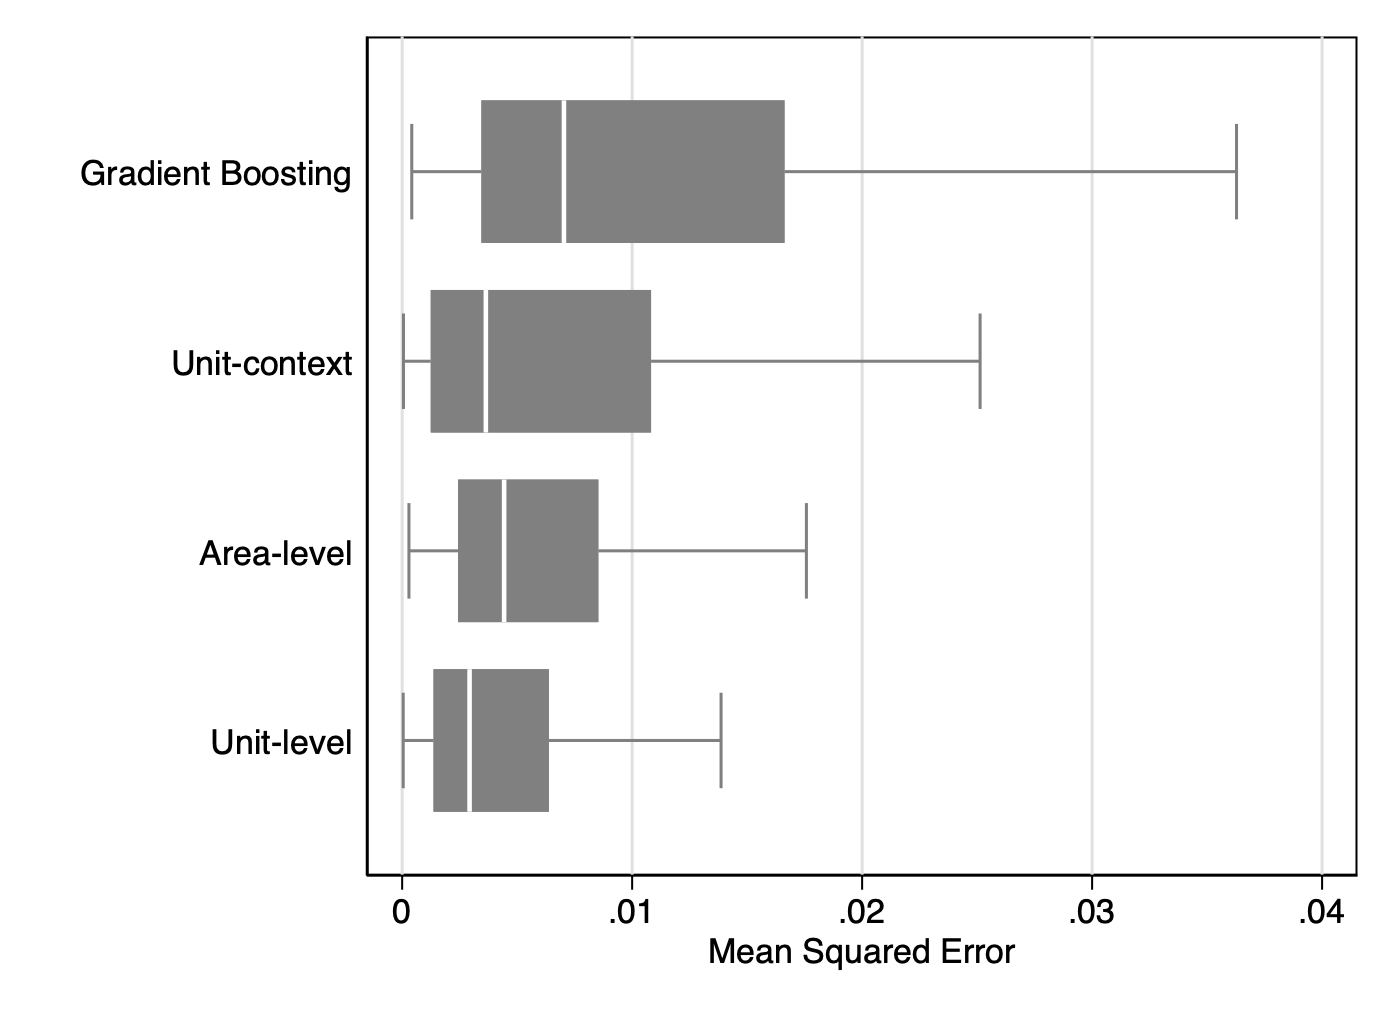
\includegraphics[scale=0.17]{Figure-1a}
%DIFDELCMD < 

%DIFDELCMD < }\hfill{}\subfloat[Unconstrained versus constrained]{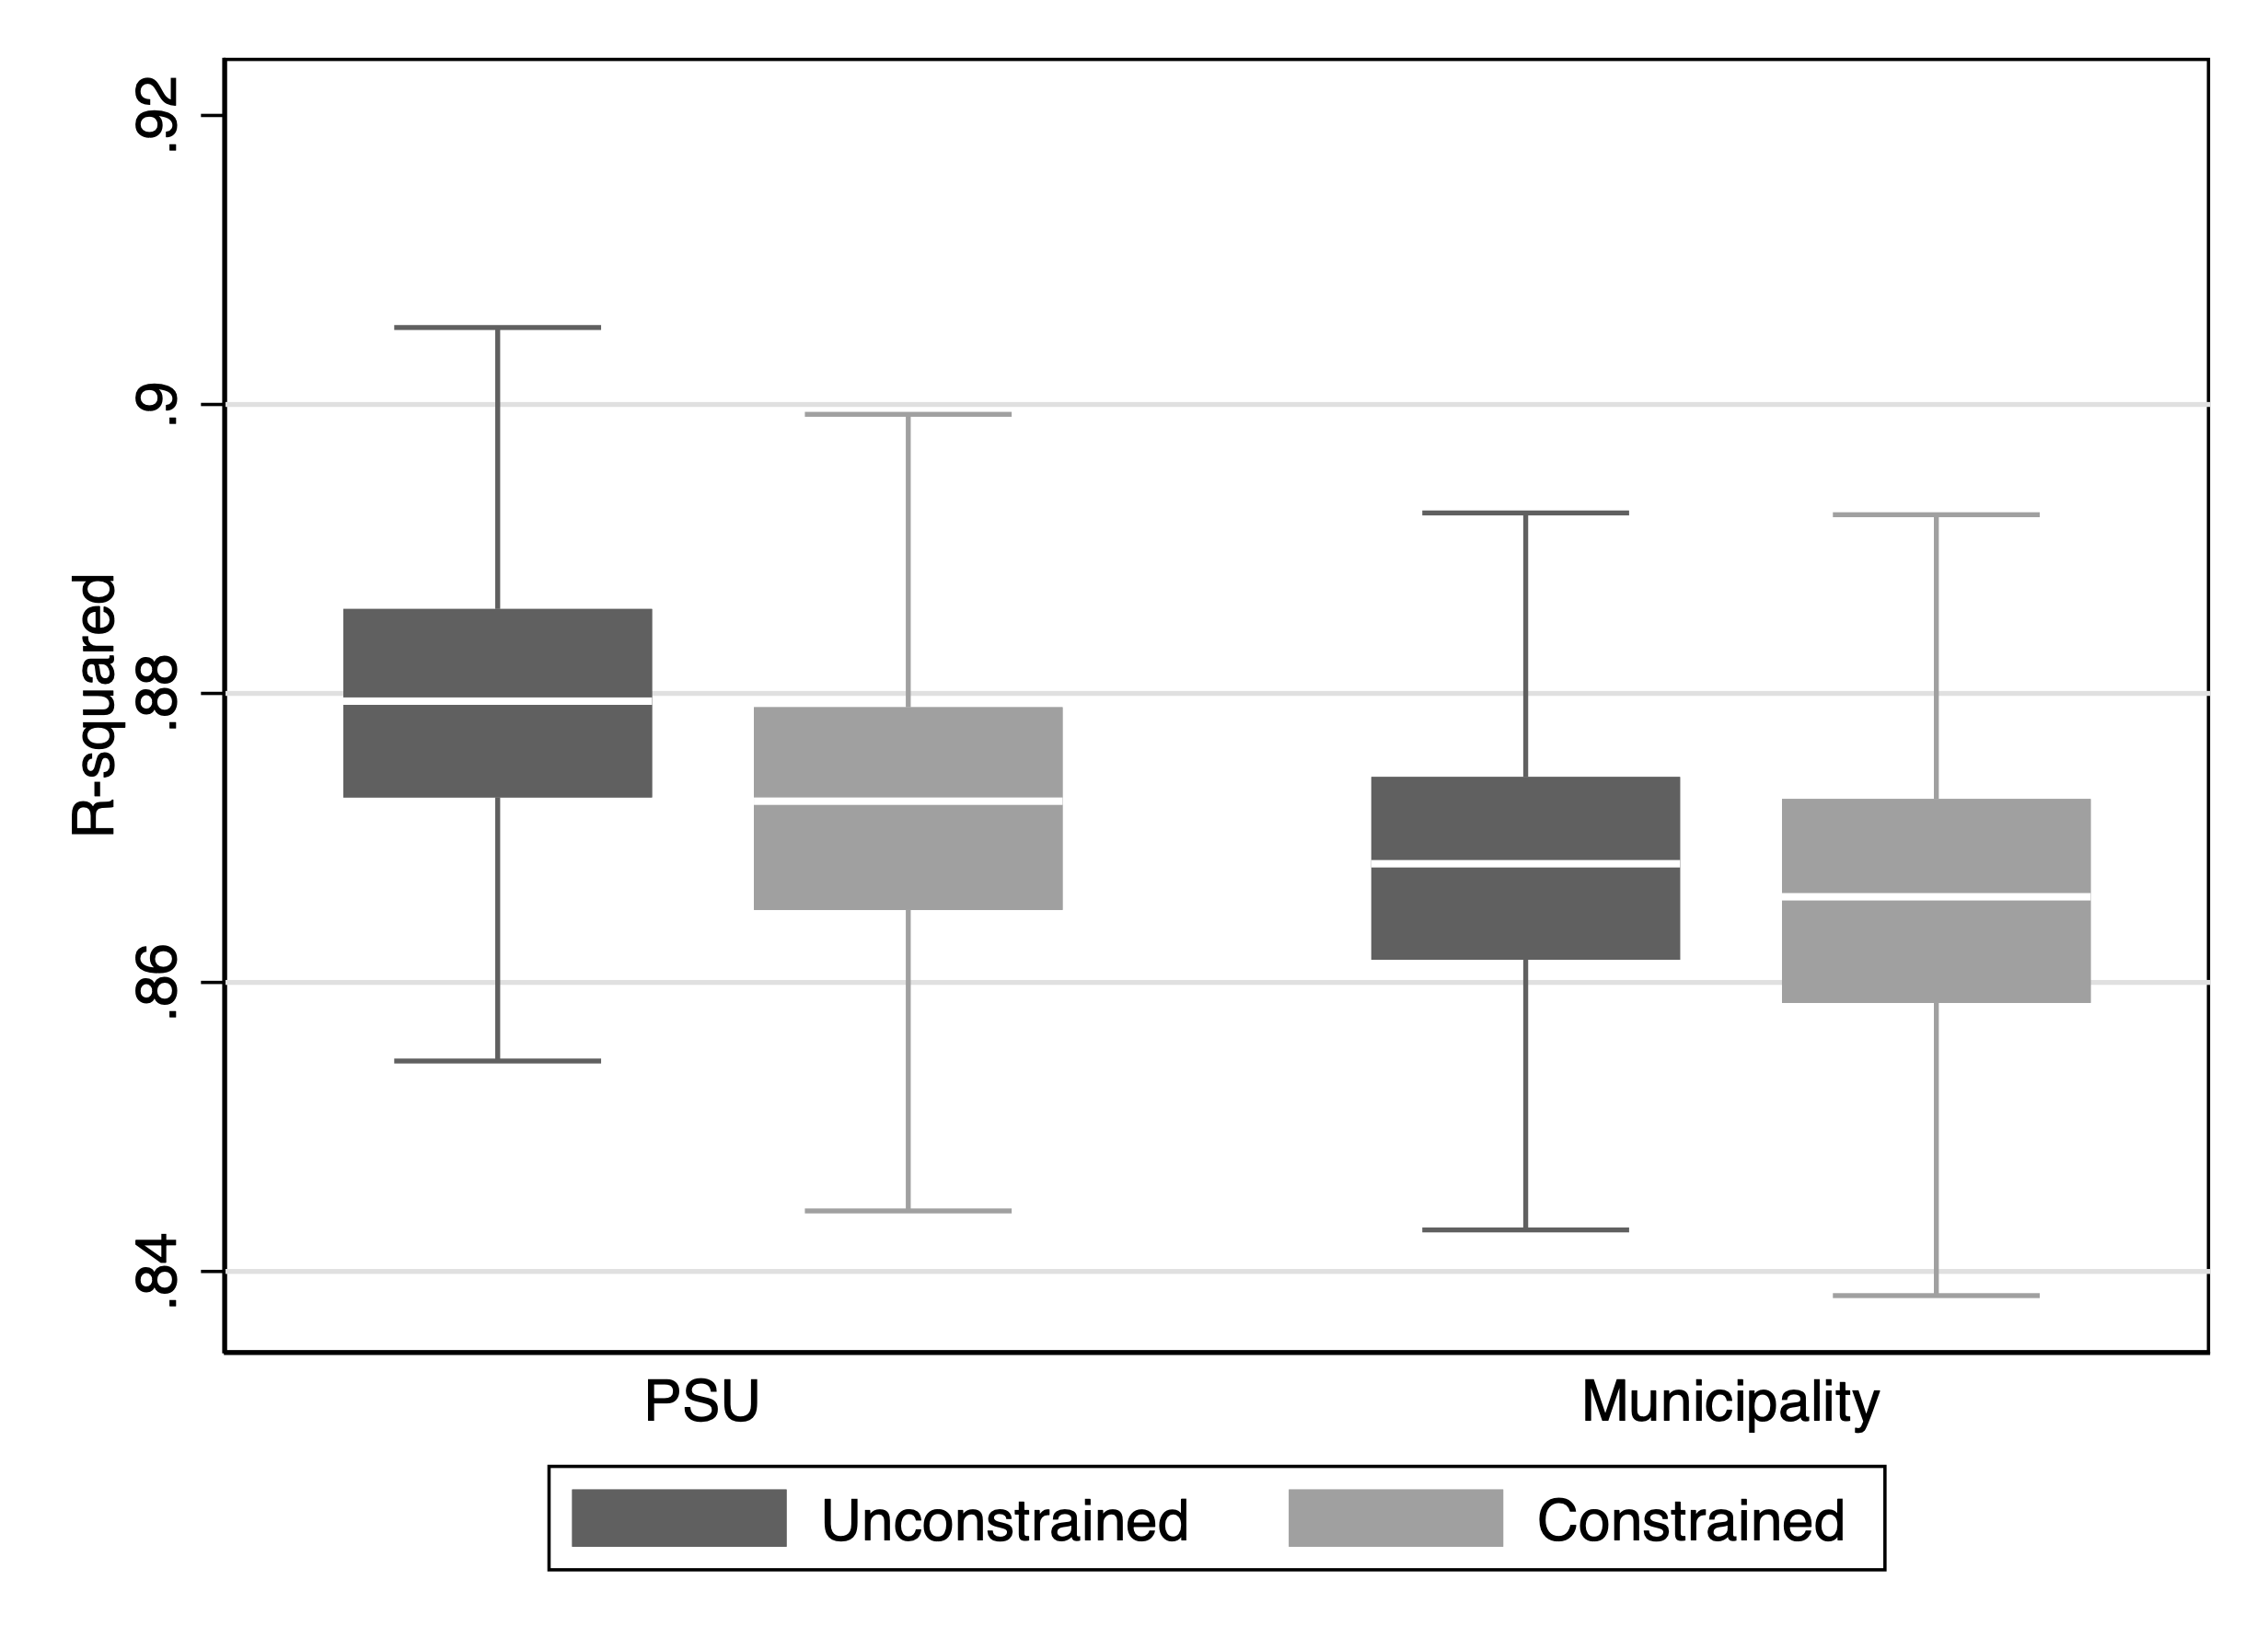
\includegraphics[scale=0.17]{Figure-1b}
%DIFDELCMD < 

%DIFDELCMD < }
%DIFDELCMD < %%%
\DIFdelendFL \DIFaddbeginFL \begin{equation}
\DIFaddFL{n_{s}=\left(\frac{\sigma_{s}}{\bar{{w}}_{s}\times\text{{RSE}}}\right)^{2}
}\end{equation}
\DIFaddendFL 

\DIFdelbeginFL %DIFDELCMD < \caption{%
{%DIFAUXCMD
\DIFdelFL{$R^{2}$ estimates at the PSU and municipality levels }%DIFDELCMD < \protect\label{fig:r2}%%%
}
%DIFAUXCMD
\DIFdelendFL \DIFaddbeginFL \DIFaddFL{where $\bar{{w}_{s}}$ and $\sigma_{s}$ represent average household
income per capita and the standard deviation of per capita income
for state $s$, respectively.
}\DIFaddendFL 

\DIFdelbeginFL %DIFDELCMD < \end{figure}
%DIFDELCMD < %%%
\DIFdelend \DIFaddbegin \DIFadd{The minimum sample size under simple random sampling must be adjusted
to account for the clustered design. The design effect due to clustering
is accounted for by estimating the intra-cluster correlation of per
capita income within each state. The correlation estimates can then
be used to adjust the above sample sizes for the clustered design
as follows:
}\DIFaddend 

\DIFdelbegin \DIFdel{Panel (a) of Figure \ref{fig:r2} presents these results and we find
evidence of considerable downward bias for both the PSU- }\DIFdelend \DIFaddbegin \begin{equation}
\DIFadd{n_{s}\times\Big[1+\rho_{s}\left(n_{sc}-1\right)\Big]
}\end{equation}

\DIFadd{where $n_{sc}$ denotes the number of households selected in cluster
$c$ within state $s$ (10 in this case) }\DIFaddend and \DIFdelbegin \DIFdel{municipality-level
models. For example, for the PSU-level model, we find that the median
``true'' $R^{2}$ is 0.88 whereas the median ``direct'' $R^{2}$
is 0.59.
Interestingly, the true $R^{2}$ tends to be higher for the PSU-level model than the municipality-level model, but the opposite
is }\DIFdelend \DIFaddbegin \DIFadd{$\rho_{s}$ is the intra-cluster
correlation of per capita income. Given the above, we can calculate
the number of clusters needed to achieve the minimum sample size for
each state and then multiply this number by 10 to find }\DIFaddend the \DIFdelbegin \DIFdel{case for the direct $R^{2}$. This suggests that model selection
based on the direct $R^{2}$ can be misleading in that the direct
$R^{2}$ incorrectly suggests that the municipality is the preferred
level of estimation.More specifically, we find that the true $R^{2}$
identifies the PSU as the preferred level of estimation for 437 of
the }\DIFdelend \DIFaddbegin \DIFadd{final sample
size. Taking these sample size requirements as given, each of our
samples is then drawn in accordance with the two-stage design.
}

\DIFadd{Specifically, the clusters within each state are selected with probability
proportional to size (without replacement) and the households within
each cluster are selected via simple random sampling. According to
this design, the inclusion probability for a given household is then
approximately:
}

\begin{equation}
\DIFadd{\frac{\tilde{{n}}_{sc}N_{s}}{\tilde{{n}}_{s}}\times\frac{n_{sc}}{\tilde{{n}}_{sc}}
}\end{equation}

\DIFadd{where $\tilde{{n}}_{sc}$ is the total number of households in cluster
$c$ within state $s$, $N_{s}$ is the number of clusters selected
in state $s$, and $\tilde{{n}}_{s}$ is the total number of households
in state $s$.}\footnote{\DIFadd{The equation used to calculate inclusion probabilities assumes sampling
with replacement, but is used here as an approximation of inclusion
probabilities under proportional selection without replacement. This
should provide a reasonable approximation in this case since there
are a relatively large number of clusters present in the frame. The
design weight for each household is simply the inverse of the inclusion
probability. In a typical survey, the design weights would be further
adjusted for nonresponse and calibrated to known population characteristics.
However, since the sampling is only a simulation exercise, there is
no nonresponse and thus no nonresponse adjustment is required. Calibration
or post-stratification could be performed, but was not implemented
to simplify the process.}} \DIFadd{Table \ref{tab:desc_stats} presents select descriptive statistics
related to the full intercensus and the }\DIFaddend 500 \DIFdelbegin \DIFdel{samples, but the
direct $R^{2}$ only selects the PSU level
for four of the 500 samples. The direct $R^{2}$ then identifies the
incorrect level of estimation for 433 of }\DIFdelend \DIFaddbegin \DIFadd{samples. We set the poverty
line at the 25th percentile of }\DIFaddend the \DIFdelbegin \DIFdel{500 samples }\DIFdelend \DIFaddbegin \DIFadd{true income distribution and the
first two rows summarize the associated poverty rates at the municipality
and PSU levels for the full dataset. The remaining rows summarize
our samples and show that we draw 23,540 households per sample (2,354
PSUs), with an average number of municipalities per sample of roughly
992. The samples thus have an average of 2.37 PSUs per municipality}\DIFaddend .

\DIFdelbegin \DIFdel{In Section \ref{sec:validation}, we discussed two other ways that the $R^{2}$ can be misleading for assessing model performance: it
is invariant to locational shifts and influenced by the variance of
the true poverty rates. Using the Mexican data, we can assess the relevance of the former issue by comparing the true $R^{2}$ to a
constrained version of the true $R^{2}$ that fixes the intercept
and coefficient to zero and one, respectively.By constraining the
$R^{2}$ in this manner, we remove its ability to adjust for systematic
differences between the poverty estimates and the true poverty rates.
Panel (b) of Figure \ref{fig:r2} presents the results and we see
that }\DIFdelend \DIFaddbegin \begin{table}
\begin{onehalfspace}
\begin{centering}
\begin{tabular}{lccccc}
\hline 
\DIFaddFL{Variable }& \DIFaddFL{Mean }& \DIFaddFL{Std. Dev. }& \DIFaddFL{Min. }& \DIFaddFL{Max. }& \DIFaddFL{Obs.}\tabularnewline
\hline 
\DIFaddFL{Municipality poverty rate (full intercensus) }& \DIFaddFL{0.30 }& \DIFaddFL{0.19 }& \DIFaddFL{0.02 }& \DIFaddFL{0.96 }& \DIFaddFL{1}\DIFaddendFL ,\DIFdelbeginFL \DIFdelFL{as expected, the unconstrained $R^{2}$ overstates the model's
performance, albeit only to a small degree.We nevertheless find that
even these small differences can lead to model selection issues. In
particular, the constrained $R^{2}$ identifies the PSU level as the appropriate level of estimation for 355 of the }\DIFdelendFL \DIFaddbeginFL \DIFaddFL{865}\tabularnewline
\DIFaddFL{PSU poverty rate (full intercensus) }& \DIFaddFL{0.23 }& \DIFaddFL{0.20 }& \DIFaddFL{0.00 }& \DIFaddFL{1.00 }& \DIFaddFL{16,297}\tabularnewline
\DIFaddFL{Observations per sample  }& \DIFaddFL{23,540 }& \DIFaddFL{0.00 }& \DIFaddFL{23,540 }& \DIFaddFL{23,540 }& \DIFaddendFL 500\DIFdelbeginFL \DIFdelFL{samples whereas
the unconstrained version, as mentioned, selects the PSU levelfor
437 out of the }\DIFdelendFL \DIFaddbeginFL \tabularnewline
\DIFaddFL{PSU per sample }& \DIFaddFL{2,354 }& \DIFaddFL{0.00 }& \DIFaddFL{2,354 }& \DIFaddFL{2,354 }& \DIFaddendFL 500\DIFdelbeginFL \DIFdelFL{samples. The commonly used unconstrained $R^{2}$
then selects the
incorrect model for 82 of }\DIFdelendFL \DIFaddbeginFL \tabularnewline
\DIFaddFL{Municipalities per sample }& \DIFaddFL{992.04 }& \DIFaddFL{11.95 }& \DIFaddFL{951 }& \DIFaddFL{1,020 }& \DIFaddFL{500}\tabularnewline
\DIFaddFL{PSU-to-municipality ratio per sample }& \DIFaddFL{2.37 }& \DIFaddFL{0.03 }& \DIFaddFL{2.31 }& \DIFaddFL{2.48 }& \DIFaddFL{500}\tabularnewline
\hline 
\end{tabular}
\par\end{centering}
\end{onehalfspace}
\caption{\DIFaddFL{Select descriptive statistics for the Mexican Intercensal Survey}\protect\label{tab:desc_stats}}

\end{table}

\DIFadd{In addition to the intercensus, INEGI has also released geo-referenced
data that is similar to }\DIFaddend the \DIFaddbegin \DIFadd{remotely-sensed covariates often used
in machine-learning applications. These geographic variables were
calculated by INEGI for the year 2015 (the same year as the intercensus)
and the municipality is the lowest administrative level for which
the covariates are available.}\footnote{\DIFadd{Technically speaking, the intercensus does not include identifiers
that provide information on geographic location below the municipality
level. We are thus only able to merge the intercensus and geo-referenced
data at the municipality level.}} \DIFadd{The geo-referenced data includes 105 indicators. Specifically, the
dataset includes information from 21 different dimensions and each
dimension is associated with five summary measures.}\footnote{\DIFadd{The 21 dimensions are as follows: enhanced vegetation index, normalized
difference vegetation index, normalized difference built-up index,
built-up index, simple ratio, atmospherically resistant vegetation
index, urban index, index of biological integrity, normalized difference
water index, modified normalized difference water index, new built-up
index, band ratio for built-up area, normalized built-up area index,
built-up area extraction index, normalized difference snow index,
visible atmospherically resistant index, soil-adjusted vegetation
index, optimized soil-adjusted vegetation index, normalized difference
moisture index, digital altitude model, and digital slope model.}} \DIFadd{For example, we summarize the atmospherically resistant vegetation
index for each municipality using the minimum, maximum, mean, sum,
and standard deviation of the index. The same procedure is applied
to all dimensions. The geo-referenced data has one major limitation,
which is that it does not include information on night-time lights,
which is a commonly-used covariate in machine-learning applications.}\footnote{\DIFadd{For examples, see \mbox{%DIFAUXCMD
\citet{jean2016combining}}\hskip0pt%DIFAUXCMD
, \mbox{%DIFAUXCMD
\citet{lee2020high}}\hskip0pt%DIFAUXCMD
,
or \mbox{%DIFAUXCMD
\citet{chi2022microestimates}}\hskip0pt%DIFAUXCMD
.}} 

\DIFadd{We thus augment the INEGI geo-referenced data with night-time lights
data produced by the Earth Observation Group (EOG). EOG uses the nightly
day/night band (DNB) low light imaging data gathered by the NASA/NOAA
Visible Infrared Imaging Radiometer Suite (VIIRS) \mbox{%DIFAUXCMD
\citep{elvidge2021annual}}\hskip0pt%DIFAUXCMD
.
To match the other geo-referenced covariates, we use the night-time
lights data from 2015, which is available at 15 arc-second resolution
(roughly }\DIFaddend 500 \DIFdelbegin \DIFdel{samples}\DIFdelend \DIFaddbegin \DIFadd{meters at the equator) and then aggregated to the municipality
level. Also like the other geo-referenced data, we summarize night-time
lights within each municipality using the minimum, maximum, mean,
sum, and standard deviation. With these additions, we then have two
alternative sets of covariates that we use in our simulations: the
geo-referenced data (including night-time lights) and the standard
set of sociodemographic covariates from the intercensus}\DIFaddend .

\DIFdelbegin %DIFDELCMD < \begin{figure}
%DIFDELCMD < \begin{centering}
%DIFDELCMD < \subfloat[Mean squared error]{\begin{centering}
%DIFDELCMD < 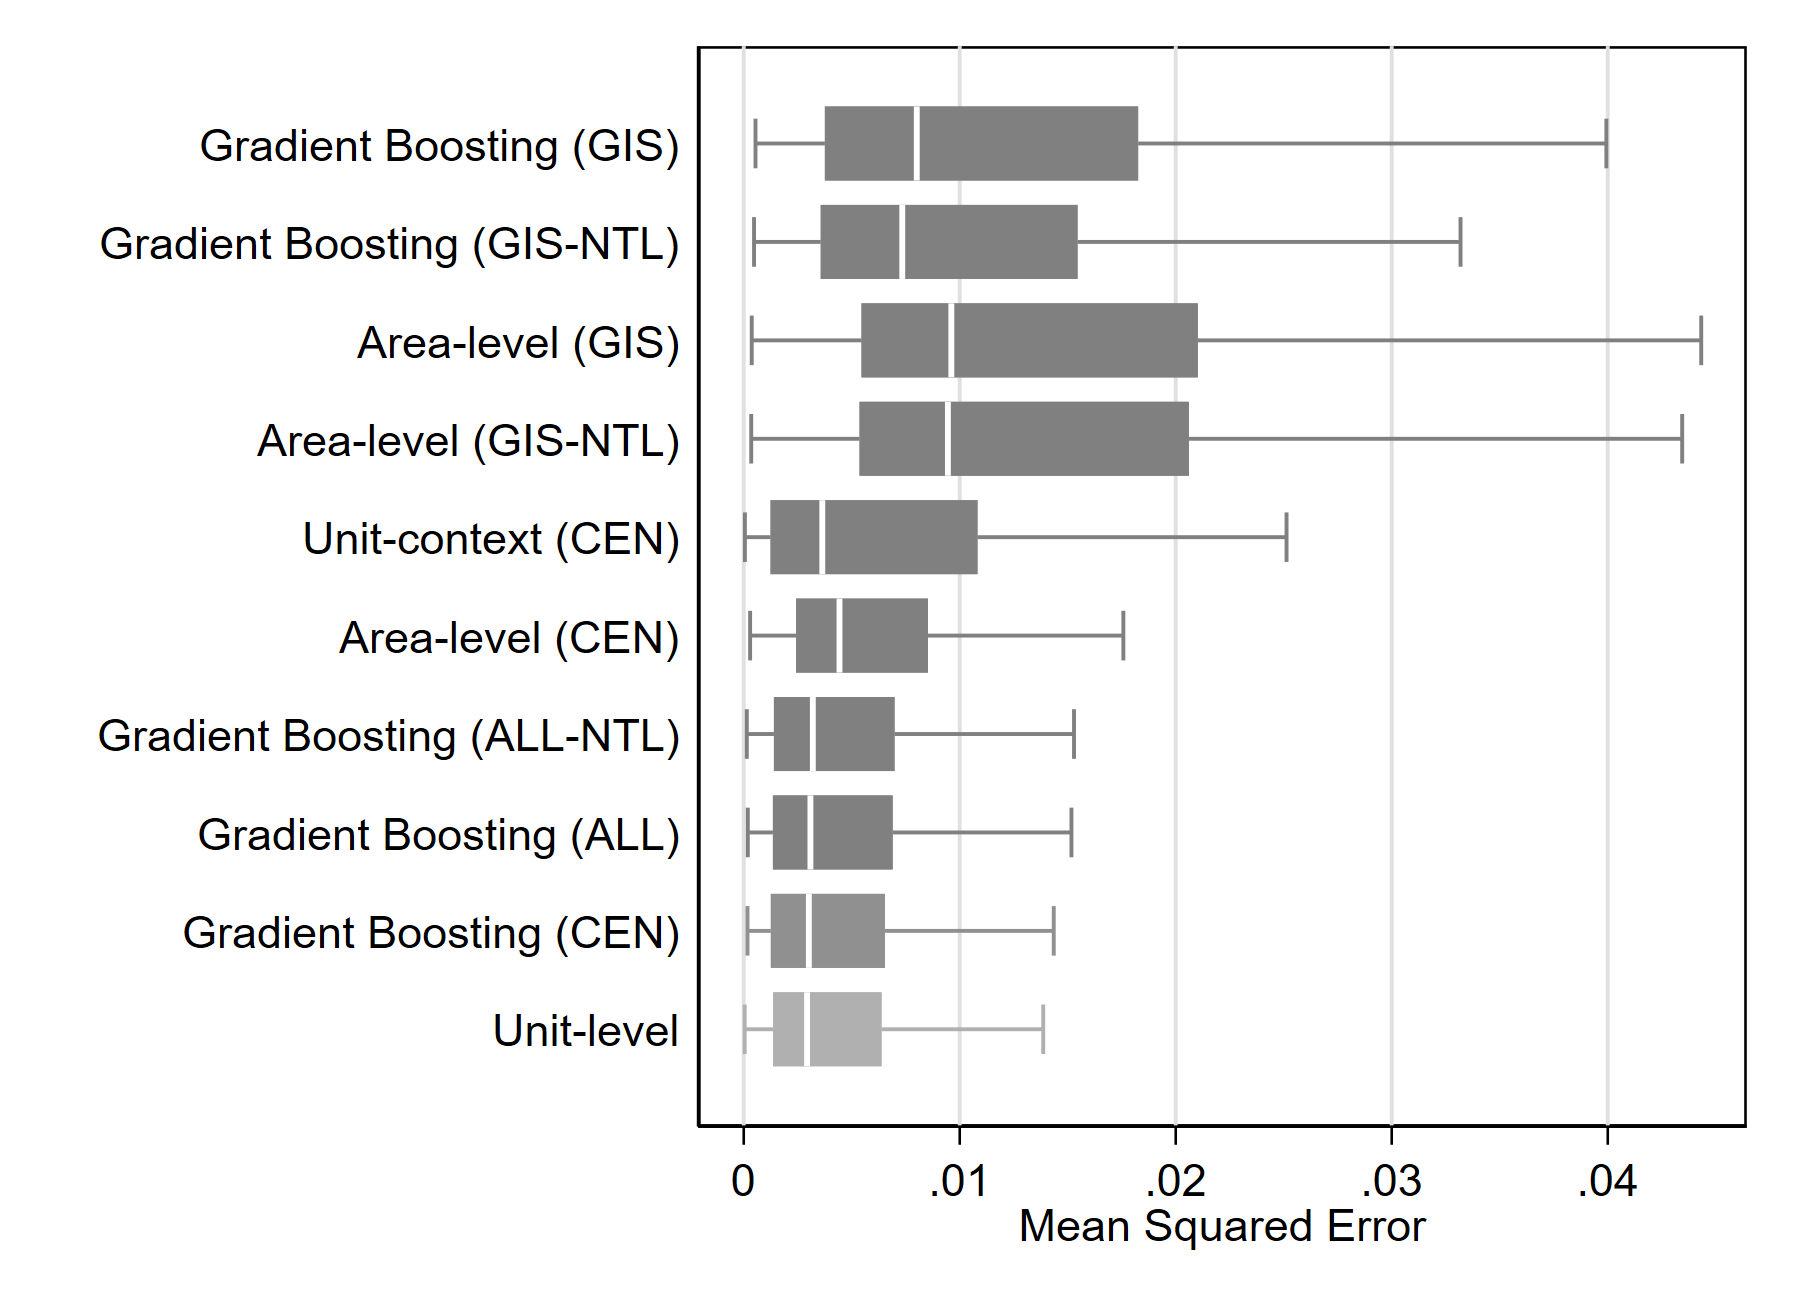
\includegraphics[scale=0.17]{Figure-2a}
%DIFDELCMD < \par\end{centering}
%DIFDELCMD < }%%%
\DIFdelFL{\hspace{0cm}}%DIFDELCMD < \subfloat[Bias]{\begin{centering}
%DIFDELCMD < 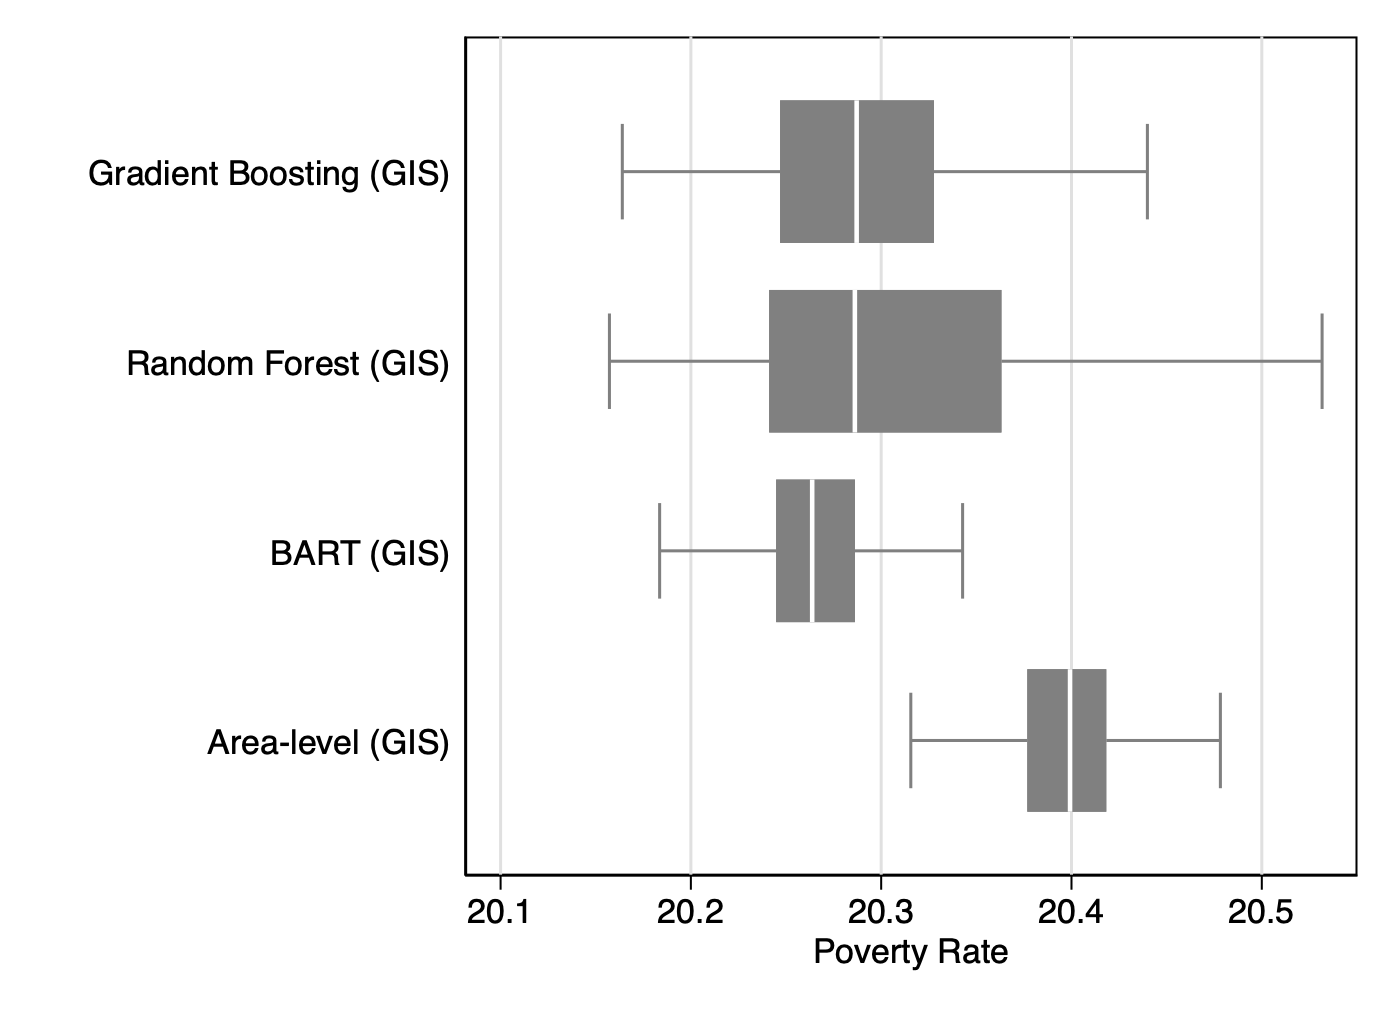
\includegraphics[scale=0.17]{Figure-2b}
%DIFDELCMD < \par\end{centering}
%DIFDELCMD < }
%DIFDELCMD < \par\end{centering}
%DIFDELCMD < \centering{}%%%
%DIFDELCMD < \caption{%
{%DIFAUXCMD
\DIFdelFL{Mean squared error and bias for select models }%DIFDELCMD < \protect\label{fig:mse}%%%
}
%DIFAUXCMD
%DIFDELCMD < \end{figure}
%DIFDELCMD < %%%
\DIFdelend \DIFaddbegin \section{\DIFadd{Results}\protect\label{sec:results}}
\DIFaddend 

\DIFdelbegin \DIFdel{Given the shortcomings of
the $R^{2}$, we have argued that the MSE
represents a better metric for model assessment. Panel }\DIFdelend \DIFaddbegin \DIFadd{Recall that our primary objective is to assess the performance of
the modern approach to poverty mapping by using the Mexican Intercensal
Survey as a ground truth. To this end, panel }\DIFaddend (a) \DIFdelbegin \DIFdel{of Figure \ref{fig:mse} thus presents our MSEresults for several alternative
models. The first three models apply gradient boosting at the municipality
level using three alternative covariate sets: geo-referenced covariates
(``GIS-MUN''), census-based covariates (``CEN-MUN''), and then
a model with all available covariates (``ALL-MUN''). The fourth
model applies gradient boosting
at the PSU level and only uses census-based
covariates (``CEN-PSU}\DIFdelend \DIFaddbegin \DIFadd{in Figure \ref{fig:mse_targeting}
presents the mean squared error (MSE) for our closest approximation
to the standard implementation of the modern approach: gradient boosting
with remotely-sensed covariates (covariates labeled ``GIS}\DIFaddend ''). \DIFdelbegin \footnote{\DIFdel{Recall that the geo-referenced covariates are only available at the
municipality level.}} %DIFAUXCMD
\addtocounter{footnote}{-1}%DIFAUXCMD
\DIFdel{The final three models are all traditional methods that we use to
}\DIFdelend \DIFaddbegin \DIFadd{We
}\DIFaddend benchmark the performance of \DIFdelbegin \DIFdel{gradient boosting. In particular, we
present }\DIFdelend \DIFaddbegin \DIFadd{this implementation against two traditional
mapping methods, namely }\DIFaddend the unit-level \DIFdelbegin \DIFdel{(obtained with CensusEB methods), unit-context
(obtained with CensusEB methods), }\DIFdelend and area-level models. \DIFdelbegin \DIFdel{We consider
three alternative implementations of the area-level model that, much
like for gradient boosting, vary the level of analysis }\DIFdelend \DIFaddbegin \DIFadd{To approximate
how these traditional methods are commonly used, each model is implemented
with census-based covariates, albeit at different levels of analysis
(covariates labeled ``CEN''). Importantly, as our initial implementations
are intended to reflect current practice, the modern and traditional
approaches differ both in terms of their statistical method }\DIFaddend and the
covariates used. \DIFdelbegin \DIFdel{For these
traditional models, all available covariates enter
the models linearly (i.e., we do not include interaction or quadratic
terms)}\DIFdelend \DIFaddbegin \DIFadd{The remainder of this section will examine how these
differences contribute to performance disparities between the two
approaches}\DIFaddend . 

\DIFdelbegin \DIFdel{One advantage of the MSE is that it can be calculated for each geographical
entity. As such, each box plot in panel }\DIFdelend \DIFaddbegin \begin{figure}
\begin{centering}
\subfloat[Mean squared error]{\begin{centering}
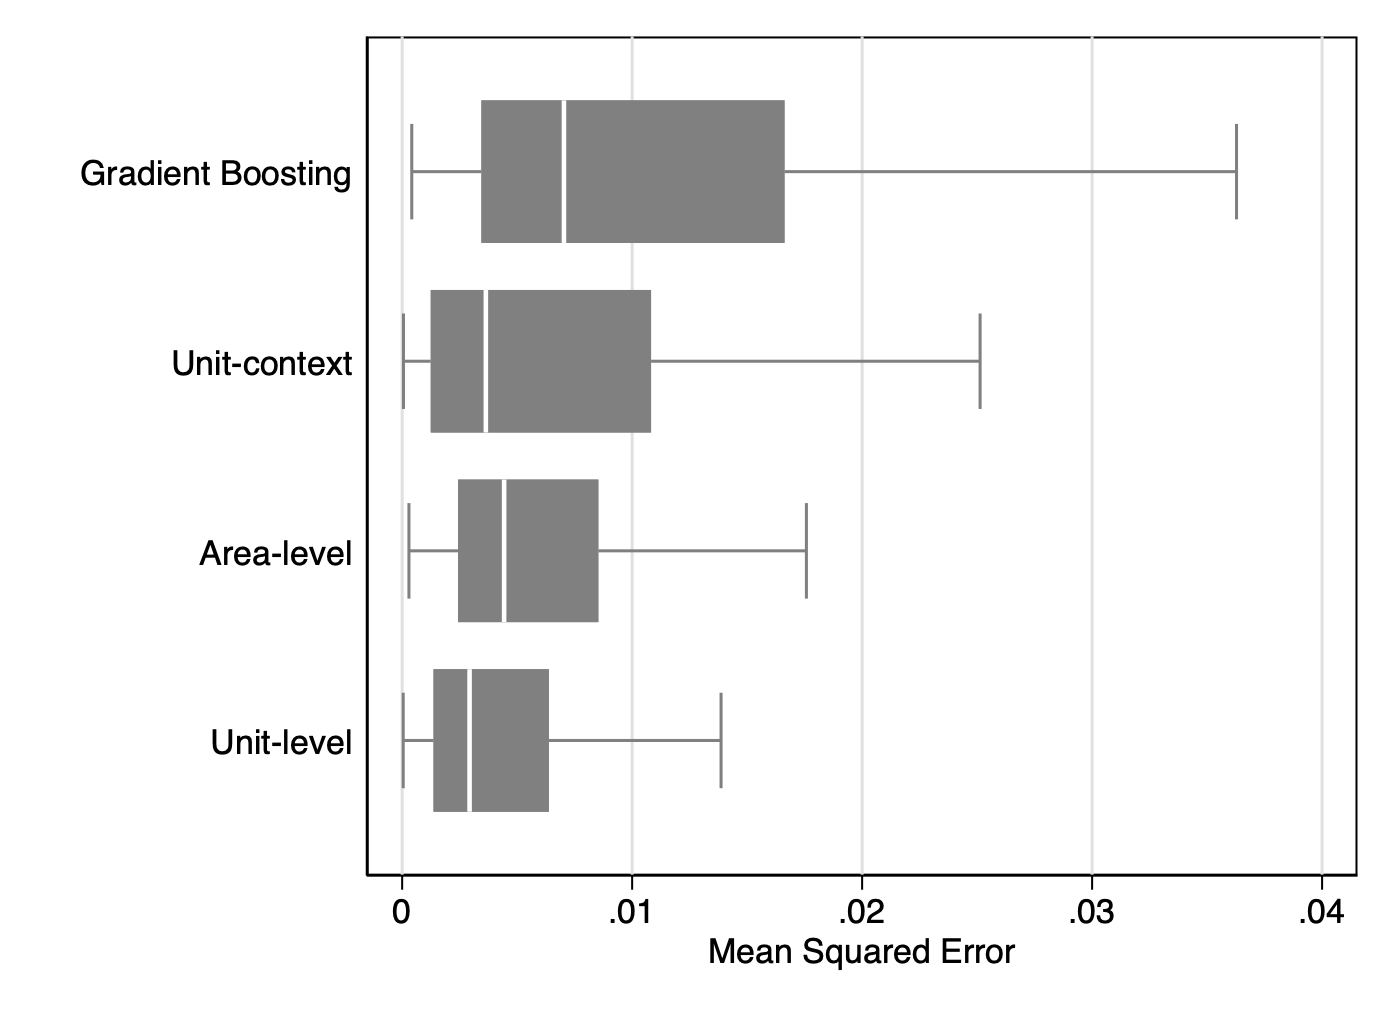
\includegraphics[scale=0.3]{Figure-1a}
\par\end{centering}
}\DIFaddFL{\hspace{0cm}}\subfloat[Targeting performance]{\begin{centering}
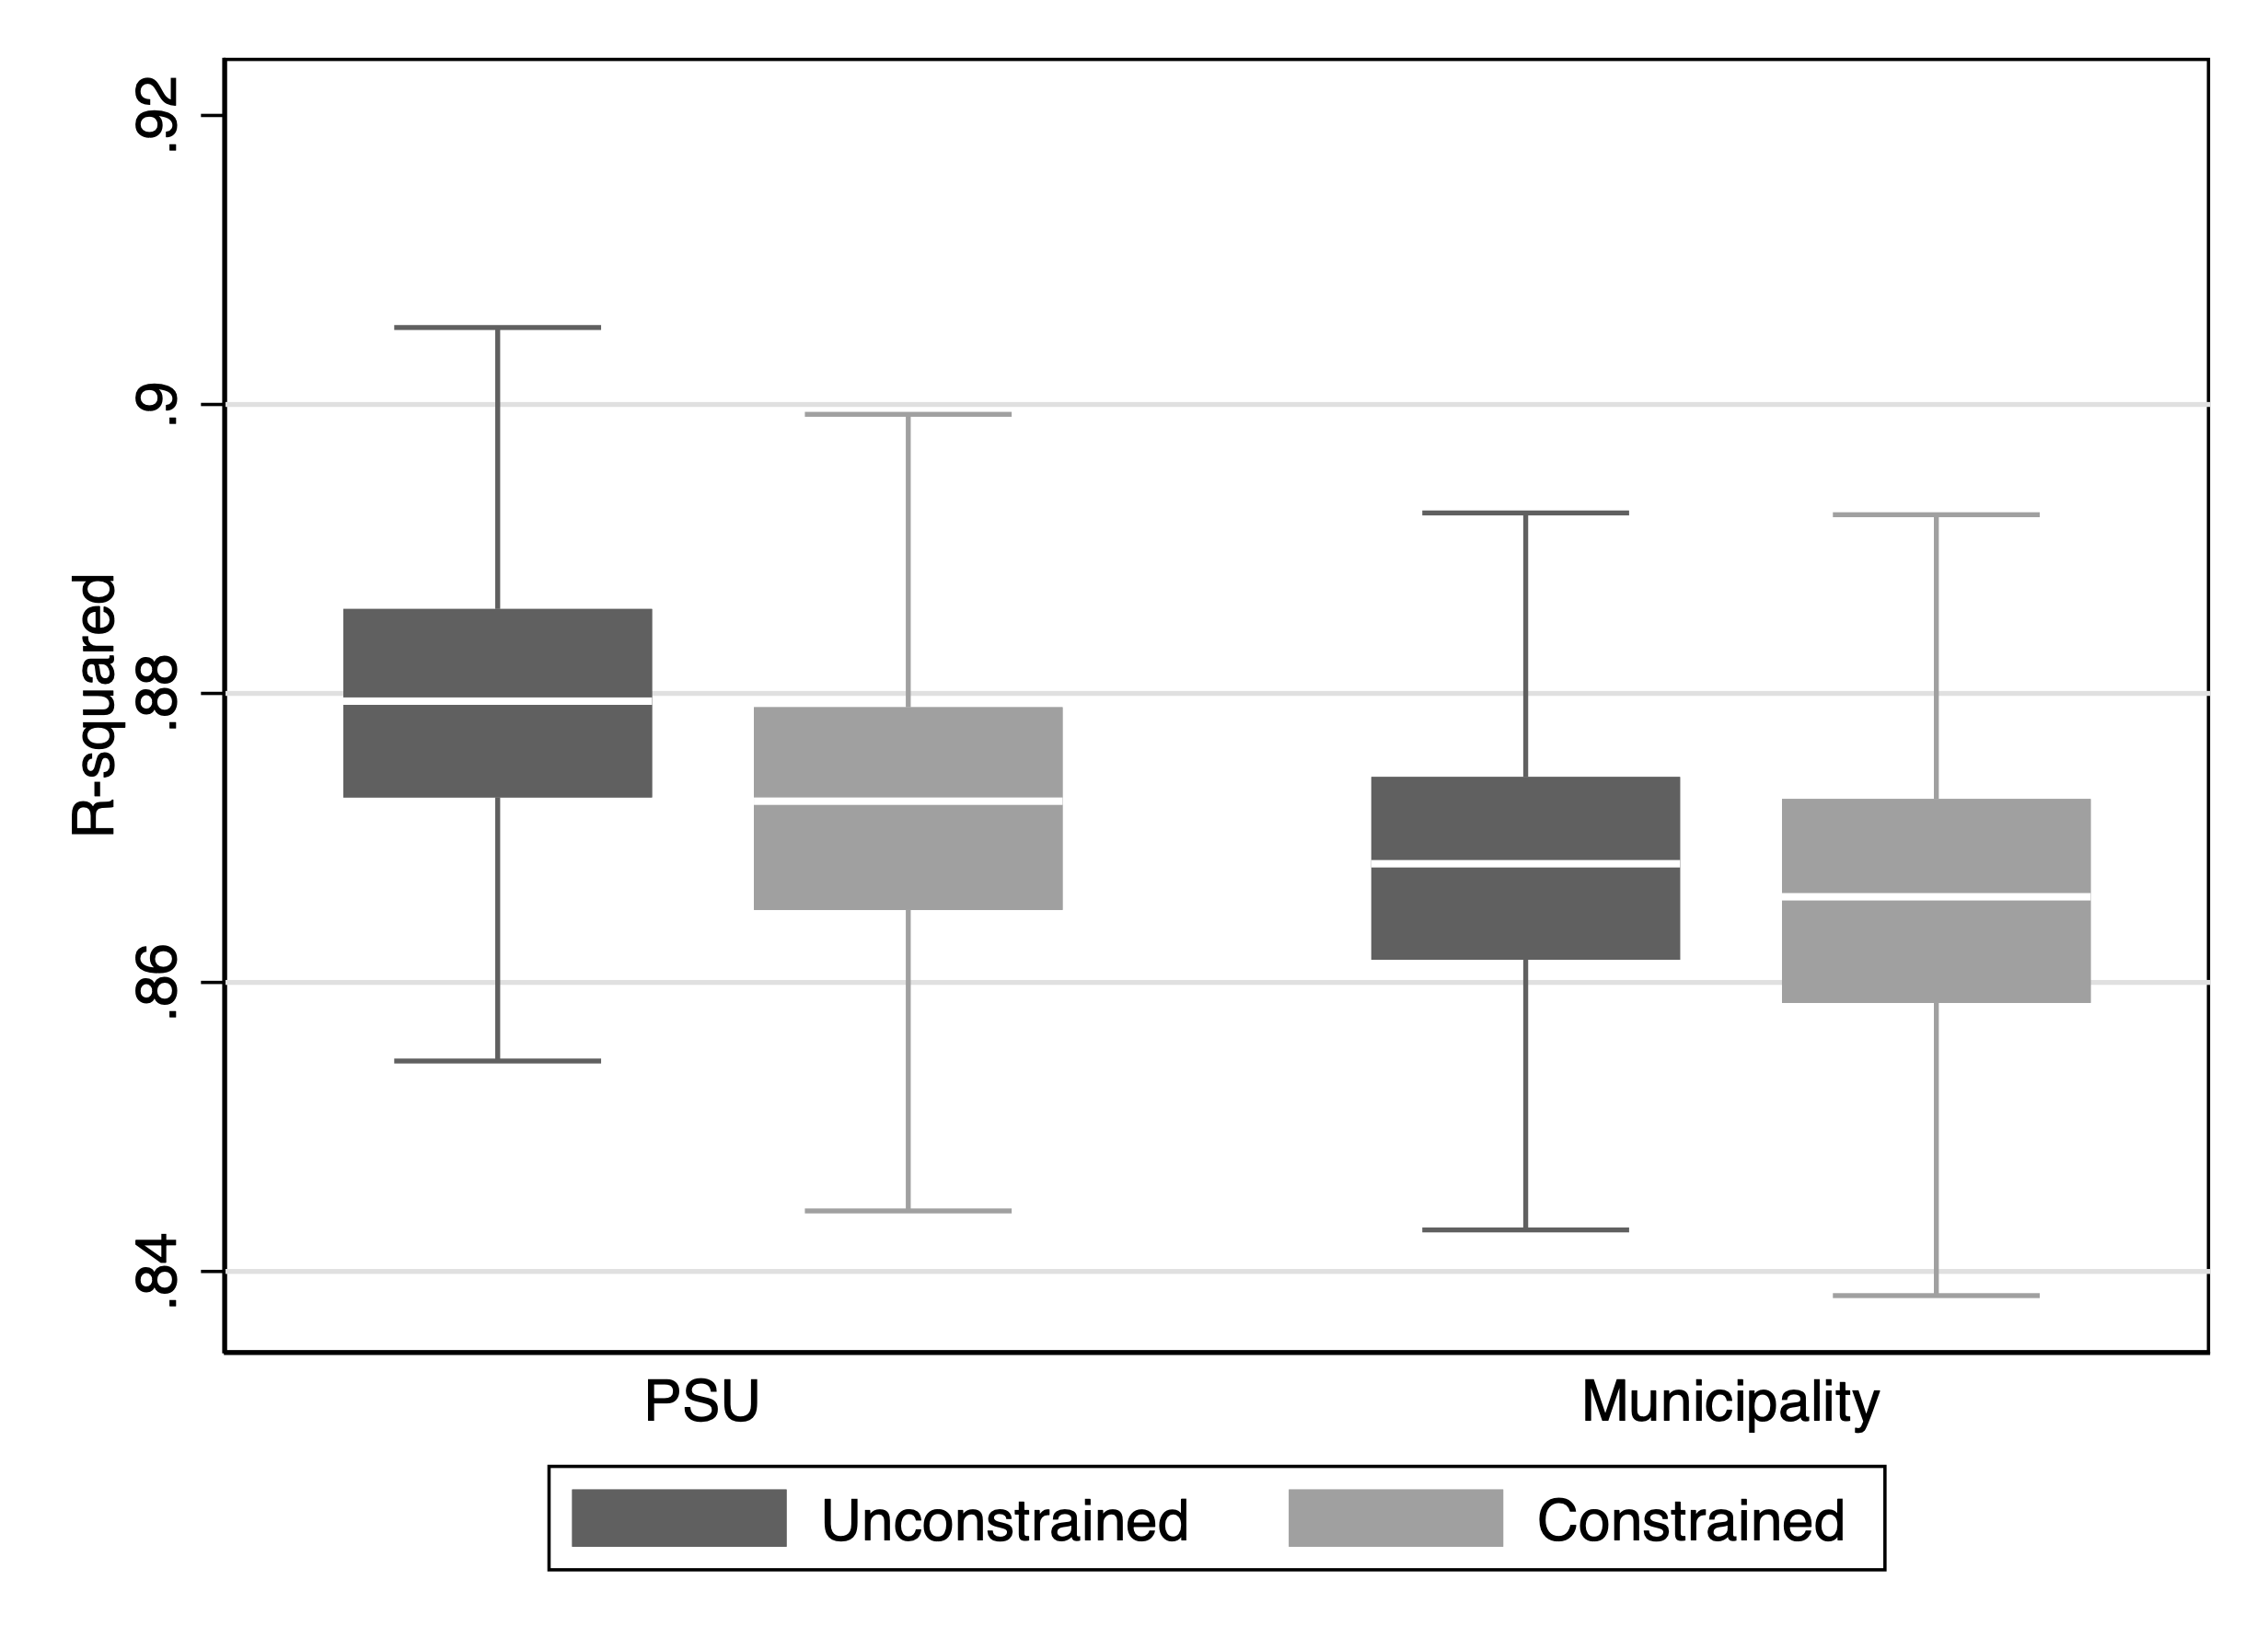
\includegraphics[scale=0.3]{Figure-1b}
\par\end{centering}
}
\par\end{centering}
\centering{}\caption{\DIFaddFL{Mean squared error and targeting performance for select implementations
}\protect\label{fig:mse_targeting}}
\end{figure}

\DIFadd{Panel }\DIFaddend (a) of Figure \DIFdelbegin \DIFdel{\ref{fig:mse}
}\DIFdelend \DIFaddbegin \DIFadd{\ref{fig:mse_targeting} shows that gradient boosting
with remotely-sensed covariates tends to have the highest MSE of the
models considered. The associated boxplot }\DIFaddend summarizes the distribution
of \DIFdelbegin \DIFdel{municipality-level MSE estimates rather
than the aggregate MSE for each sample }\DIFdelend \DIFaddbegin \DIFadd{MSE values across all municipalities }\DIFaddend (i.e., the results are based
on Eq. {[}\ref{eq:mseg}{]}) \DIFdelbegin \DIFdel{. It is useful to first consider how gradient
boosting performs relative to the traditional models when using the
same census-based covariates. In this case, the gradient boosting
implementations at the municipality and PSU levels achieve median MSE values of 0.003 }\DIFdelend and \DIFdelbegin \DIFdel{0.002, respectively. In }\DIFdelend \DIFaddbegin \DIFadd{indicates that the gradient-boosting
model achieves a median MSE of 0.007. The corresponding root MSE is
approximately 0.08, meaning that the median municipality's error is
roughly eight percentage points. By }\DIFaddend contrast, the \DIFdelbegin \DIFdel{\textquotedblleft gold standard\textquotedblright{} }\DIFdelend \DIFaddbegin \DIFadd{``gold standard''
}\DIFaddend unit-level \DIFdelbegin \DIFdel{model }\DIFdelend achieves a median MSE of 0.003\DIFdelbegin \DIFdel{. The remaining traditional methods that use census-based
covariates all achieve }\DIFdelend \DIFaddbegin \DIFadd{, which is roughly 40 percent
that of the gradient-boosting model. The area-level model performs
similarly to the unit-level model, with }\DIFaddend a median MSE of \DIFdelbegin \DIFdel{roughly }\DIFdelend 0.004. \DIFdelbegin \DIFdel{These results
suggest that , when using the same data, gradient boosting performs
comparably (if not better) than the unit-level model and better than
the unit-context and area-level models . Given that traditional small
area methods tend to make more use of the data at hand, the performance
of gradient boosting is somewhat surprising. It may be due to the fact that gradient boosting accommodates more flexible functional
forms or it may be something specific to the data at hand.
}\DIFdelend \DIFaddbegin \DIFadd{The
fact that the area-level model outperforms the gradient-boosting model
is particularly notable, as both of these models were developed for
use in off-census years and are thus direct competitors.
}\DIFaddend 

\DIFdelbegin \DIFdel{Recall, however, that the machine-learning approach to poverty mapping
most commonly uses remotely-sensed covariates rather than census-based
covariates. The gradient boosting model with geo-referenced covariates (``GIS-MUN'') is our closest approximation to this standard implementation.
This model }\DIFdelend \DIFaddbegin \DIFadd{Panel (b) of Figure \ref{fig:mse_targeting} considers the targeting
performance of the alternative models and shows a similar result.
For these simulations, we have set the poverty line at the 25th percentile
of the (pre-transfer) per capita income distribution, which means
that the baseline poverty rate is 25 percent. The poverty rate falls
to 19.9 percent when transfers are delivered to municipalities according
to their true poverty rate. Across 500 simulations, we find that gradient
boosting with remotely-sensed covariates }\DIFaddend achieves a median \DIFdelbegin \DIFdel{MSE of 0.008 (with a root MSE of about
0.09), meaning that the median municipality's error is roughly nine
percentage points. It is useful to compare these results to those
from the unit-context and area-level models given that these models
are direct competitors to machine learning.
The unit-context model
and the area-level models with census covariates all achieve median MSE values of 0.004, }\DIFdelend \DIFaddbegin \DIFadd{poverty
rate of 20.29, which is close to the benchmark rate of 19.9 percent.
The two traditional methods nevertheless outperform the gradient-boosting
model. The unit-level model achieves a median poverty rate of 20 percent
}\DIFaddend whereas the area-level model \DIFdelbegin \DIFdel{using geo-referenced
covariates }\DIFdelend achieves a median \DIFdelbegin \DIFdel{MSE of 0.01. With the exception of the area-level model based on geo-referenced covariates,we thus find
that the standard implementation performs considerably worse than
the traditional methods that are also feasible in off-census years.
}\DIFdelend \DIFaddbegin \DIFadd{rate of 20.04. The
traditional approach thus outperforms the modern approach by about
0.3 percentage points, which in a country the size of Mexico corresponds
to about 360,000 additional people escaping poverty.}\footnote{\DIFadd{Mexico's population was about 120 million in 2015, which is the year
that the Mexican Intercensal Survey was conducted.}}
\DIFaddend 

\DIFdelbegin \DIFdel{The bias associated with poverty estimates is especially important
due to }\DIFdelend \DIFaddbegin \DIFadd{As mentioned, there are two primary differences between the traditional
and modern approaches that could explain these performance disparities:
the statistical method and the covariates used. We first examine whether
using an alternative statistical method could improve upon the performance
of our initial implementation of the modern approach. Figure \ref{fig:alt_methods}
presents MSE and targeting results for four alternative statistical
methods where each uses the same, remotely-sensed covariates in order
to isolate the influence of the method. In addition to gradient boosting,
we consider two leading non-parametric competitors (i.e., random forest
and Bayesian additive regression trees) and the leading parametric
competitor (i.e., }\DIFaddend the \DIFdelbegin \DIFdel{policy relevance of understanding absolute living standards. In panel (b) of Figure \ref{fig:mse}, we thus present box plots for
the municipality-level bias estimates associated with each model(see
Eq.}%DIFDELCMD < {[}%%%
\DIFdel{\ref{eq:mseg}{]} for the bias-variance decomposition of the
MSE). The median bias for all models is approximately zero, with the possible exception of the unit-context model and the }\DIFdelend \DIFaddbegin \DIFadd{area-level model).}\footnote{\DIFadd{In terms of non-parametric models, both random forests and Bayesian
additive regression trees are quite popular and have been shown to
perform comparably to, and sometimes better than, gradient boosting.
For example, see \mbox{%DIFAUXCMD
\citet{chipman2010bart}}\hskip0pt%DIFAUXCMD
. }} \DIFadd{We find that the alternative methods do not produce any substantive
performance gains. In particular, the two alternative non-parametric
methods perform similarly to gradient boosting whereas the parametric,
}\DIFaddend area-level model \DIFdelbegin \DIFdel{estimated at the PSU level.}\DIFdelend \DIFaddbegin \DIFadd{tends to perform slightly worse when using the same
covariates.}\DIFaddend \footnote{\DIFdelbegin \DIFdel{The same issue for unit-context models is highlighted by \mbox{%DIFAUXCMD
\citet{corral2021map}
}\hskip0pt%DIFAUXCMD
and \mbox{%DIFAUXCMD
\citet{corral2022guidelines}}\hskip0pt%DIFAUXCMD
}\DIFdelend \DIFaddbegin \DIFadd{Bayesian additive regression trees perform slightly better than gradient
boosting, but the performance gains are not large}\DIFaddend . \DIFaddbegin \DIFadd{For example, in
terms of targeting performance, gradient boosting achieves a median
poverty rate of 20.29 whereas the Bayesian method achieves a median
rate of 20.26. }\DIFaddend }
\DIFdelbegin \DIFdel{Perhaps the more interesting result is that the bias estimates from
the gradient boosting model with geo-referenced covariates exhibits
considerable variation, with minimum and maximum biases reaching -0.43
and 0.43}\DIFdelend \DIFaddbegin 

\begin{figure}
\begin{centering}
\subfloat[Mean squared error]{\begin{centering}
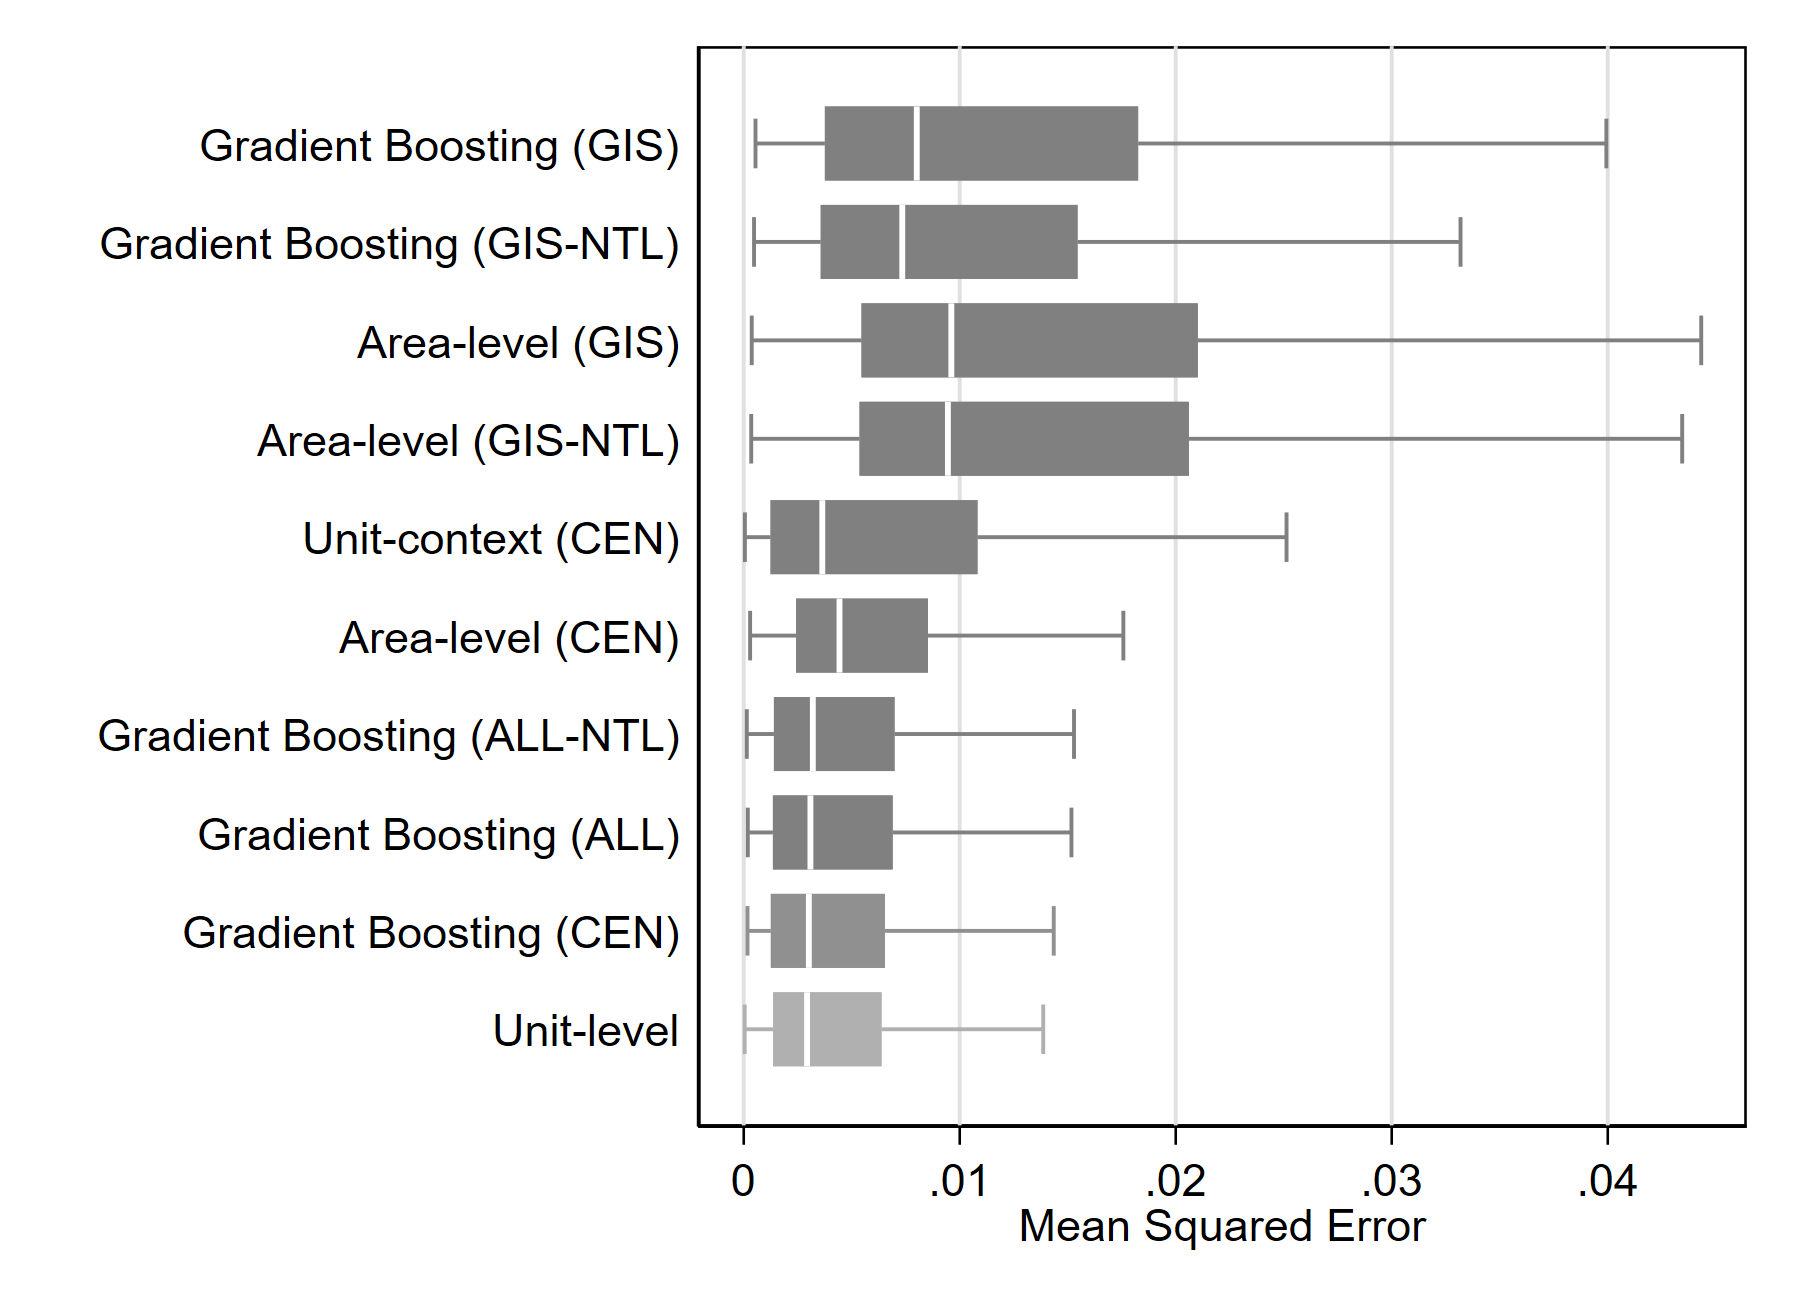
\includegraphics[scale=0.3]{Figure-2a}
\par\end{centering}
}\DIFaddFL{\hspace{0cm}}\subfloat[Targeting performance]{\begin{centering}
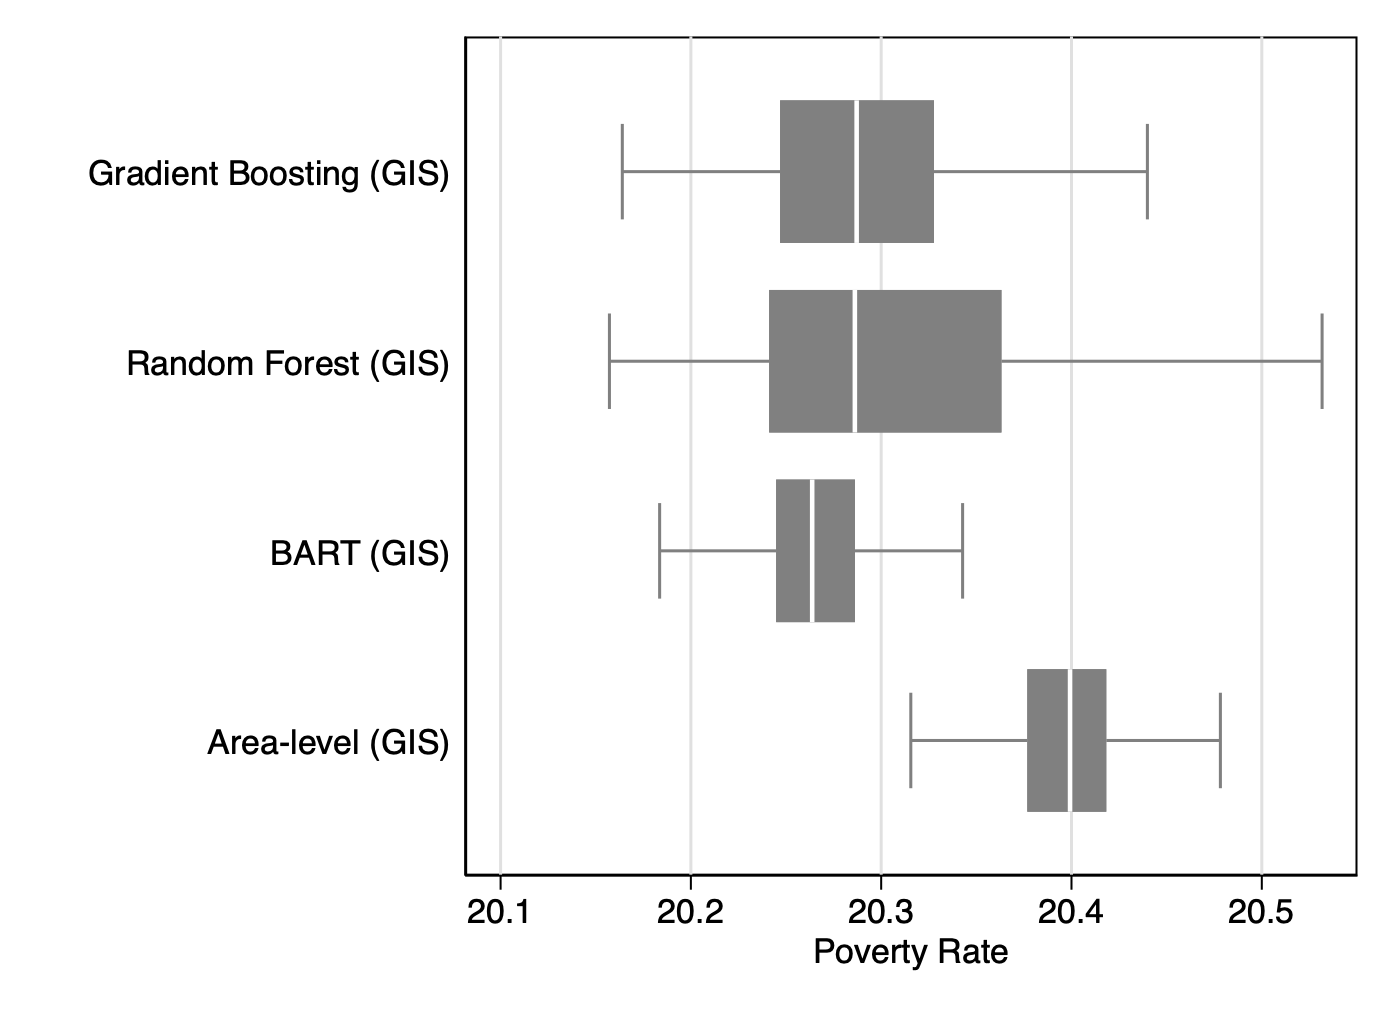
\includegraphics[scale=0.3]{Figure-2b}
\par\end{centering}
}
\par\end{centering}
\centering{}\caption{\DIFaddFL{Mean squared error and targeting performance for alternative statistical
methods }\protect\label{fig:alt_methods}}
\end{figure}

\DIFadd{By contrast, Figure \ref{fig:alt_covariates} shows that implementing
gradient boosting with census-based covariates leads to notable performance
gains. The first two boxplots in panels (a) and (b) present the results
for gradient boosting with remotely-sensed and census-based covariates}\DIFaddend ,
respectively. \DIFdelbegin \DIFdel{That is, the standard implementation with
}\DIFdelend \DIFaddbegin \DIFadd{As a benchmark, we plot similar results for the area-level
model. Recall that when using }\DIFaddend remotely-sensed covariates\DIFdelbegin \DIFdel{is severely biased for some municipalities, even though its median bias is approximately zero. All other models, including the competing unit-context and }\DIFdelend \DIFaddbegin \DIFadd{, gradient
boosting achieves a median MSE of 0.007 and a median poverty rate
of 20.29. With census-based covariates, the median MSE falls to 0.003
and the median poverty rate falls to 20.02. Importantly, gradient
boosting with census-based covariates slightly outperforms the }\DIFaddend area-level
\DIFdelbegin \DIFdel{models, exhibit
much less variation. }\DIFdelend \DIFaddbegin \DIFadd{model, which achieves a median MSE of 0.004 and a median poverty rate
of 20.04 when using the same covariates. The under-performance of
the modern approach is thus largely driven by the remotely-sensed
covariates.
}\DIFaddend 

\begin{figure}
\begin{centering}
\DIFdelbeginFL %DIFDELCMD < 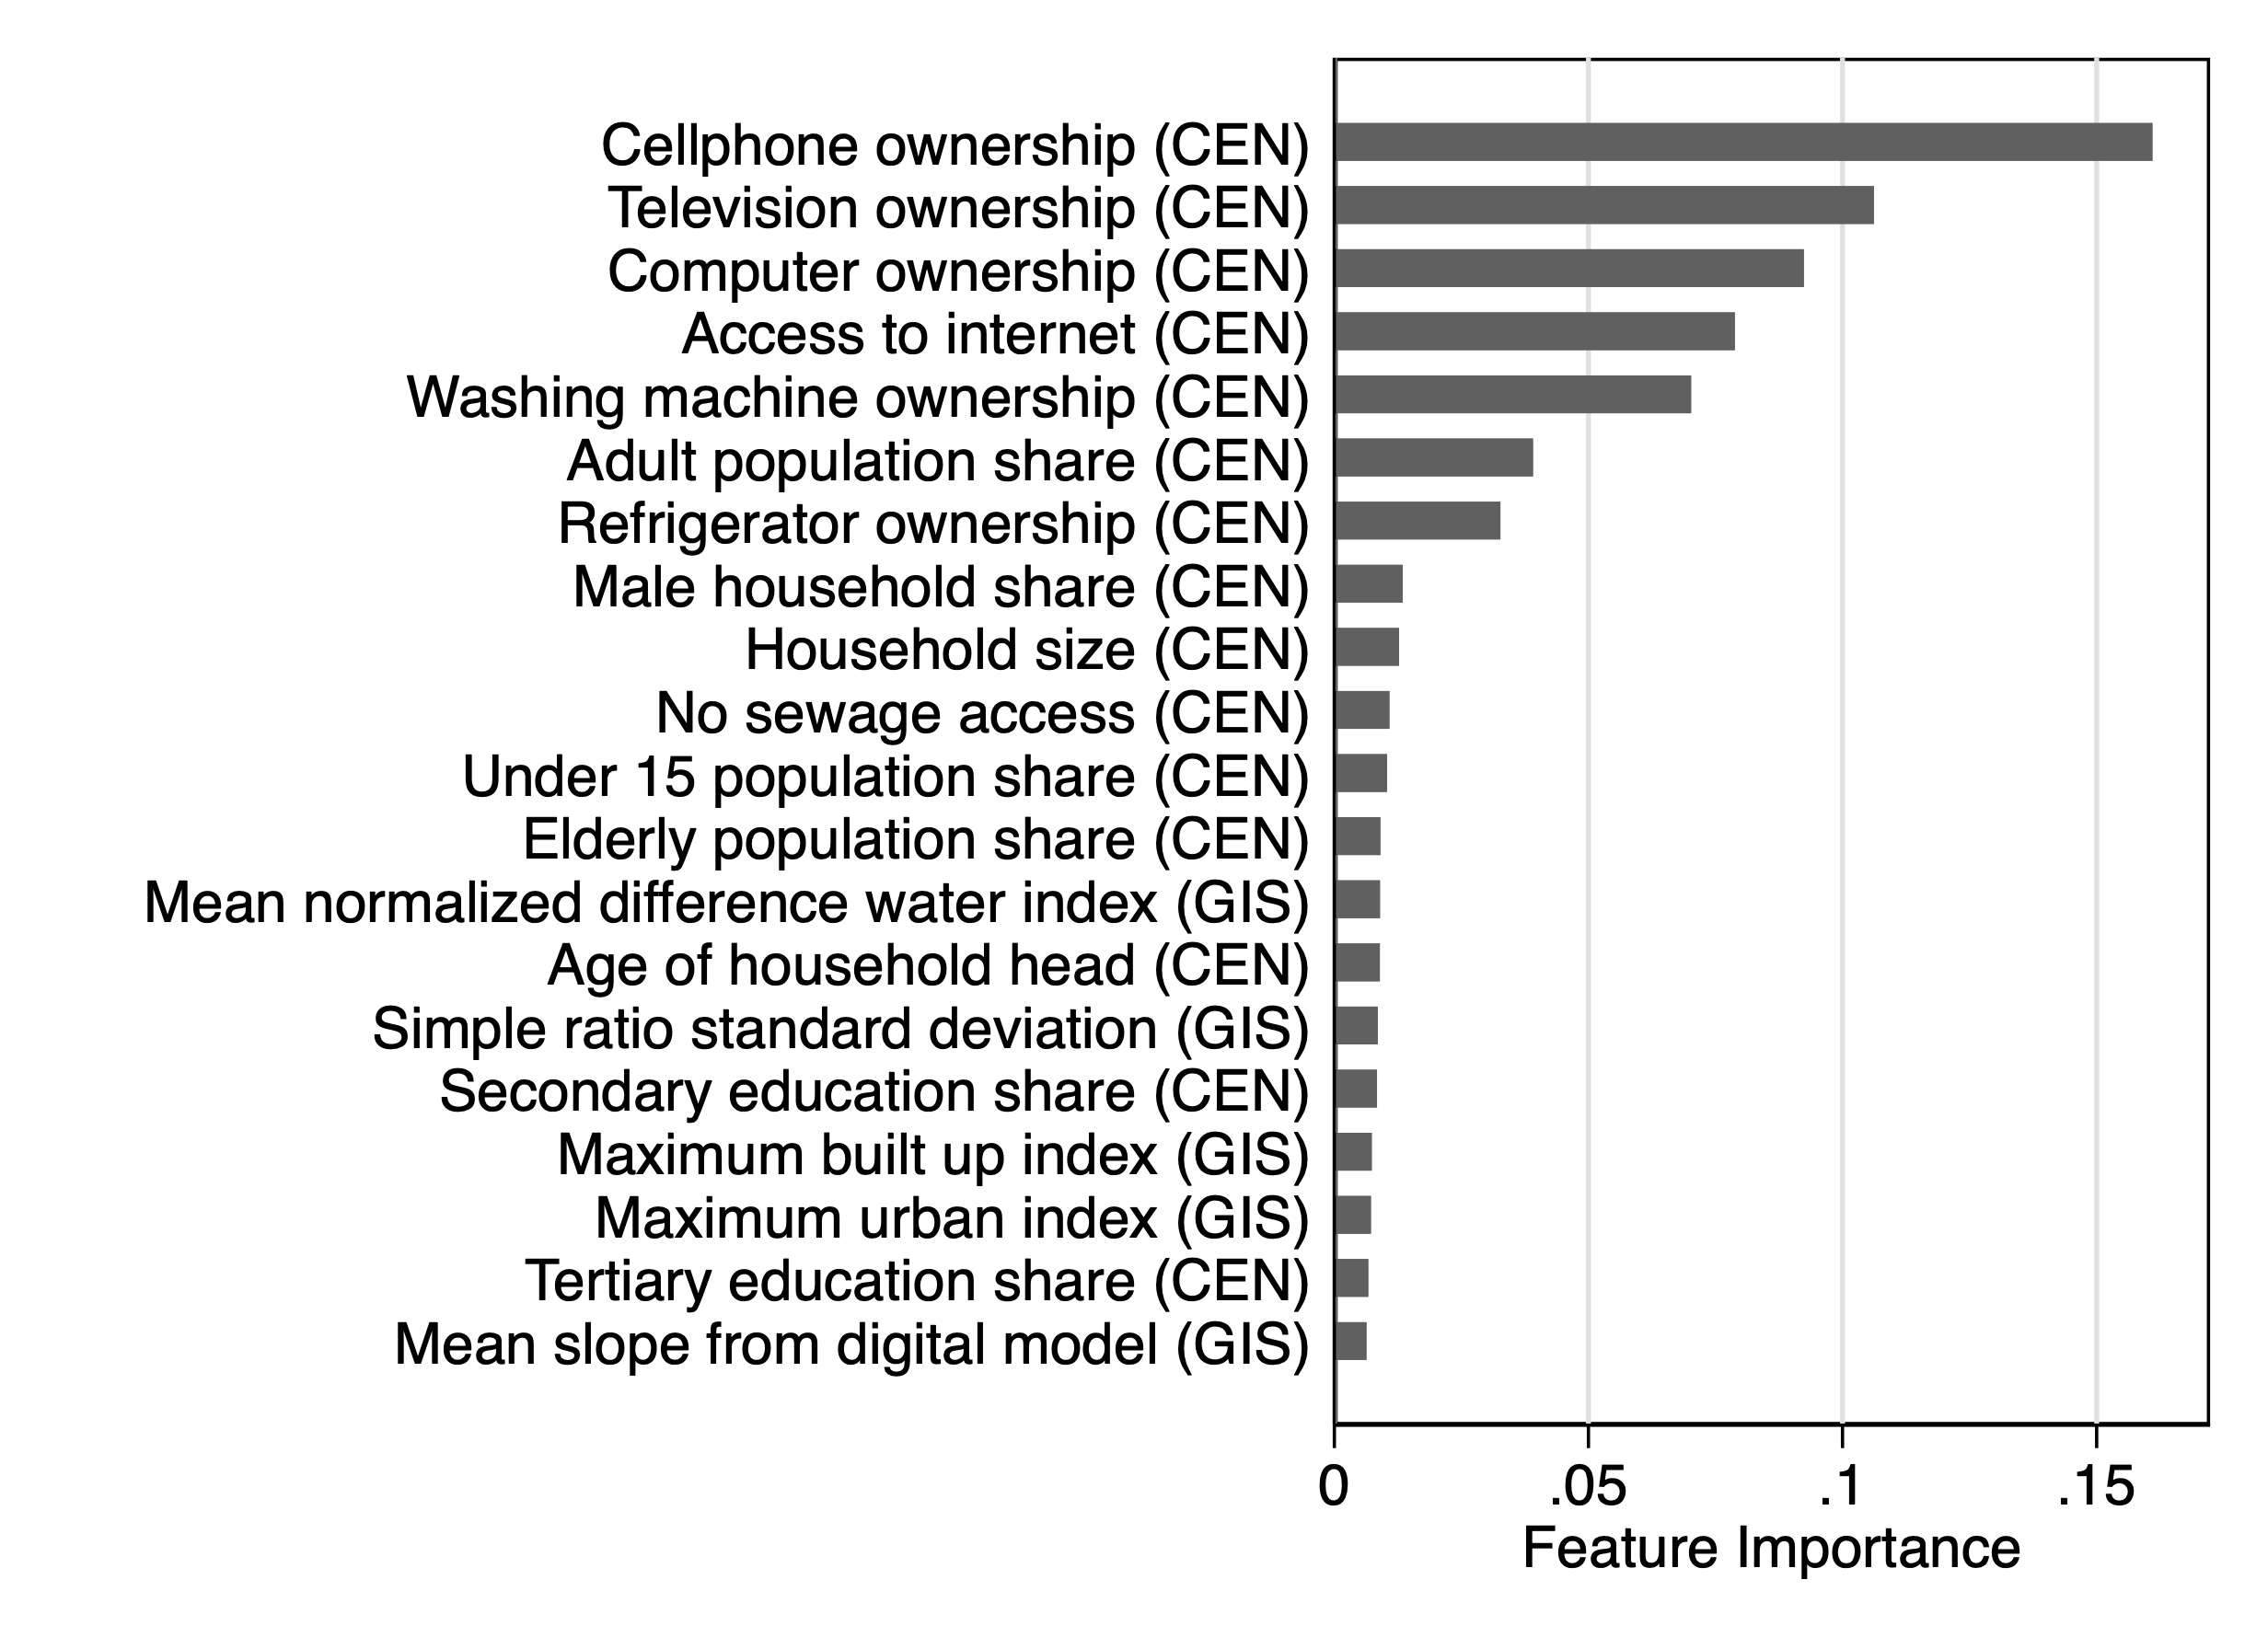
\includegraphics[scale=0.25]{Figure-3.png}
%DIFDELCMD < %%%
\DIFdelendFL \DIFaddbeginFL \subfloat[Mean squared error]{\begin{centering}
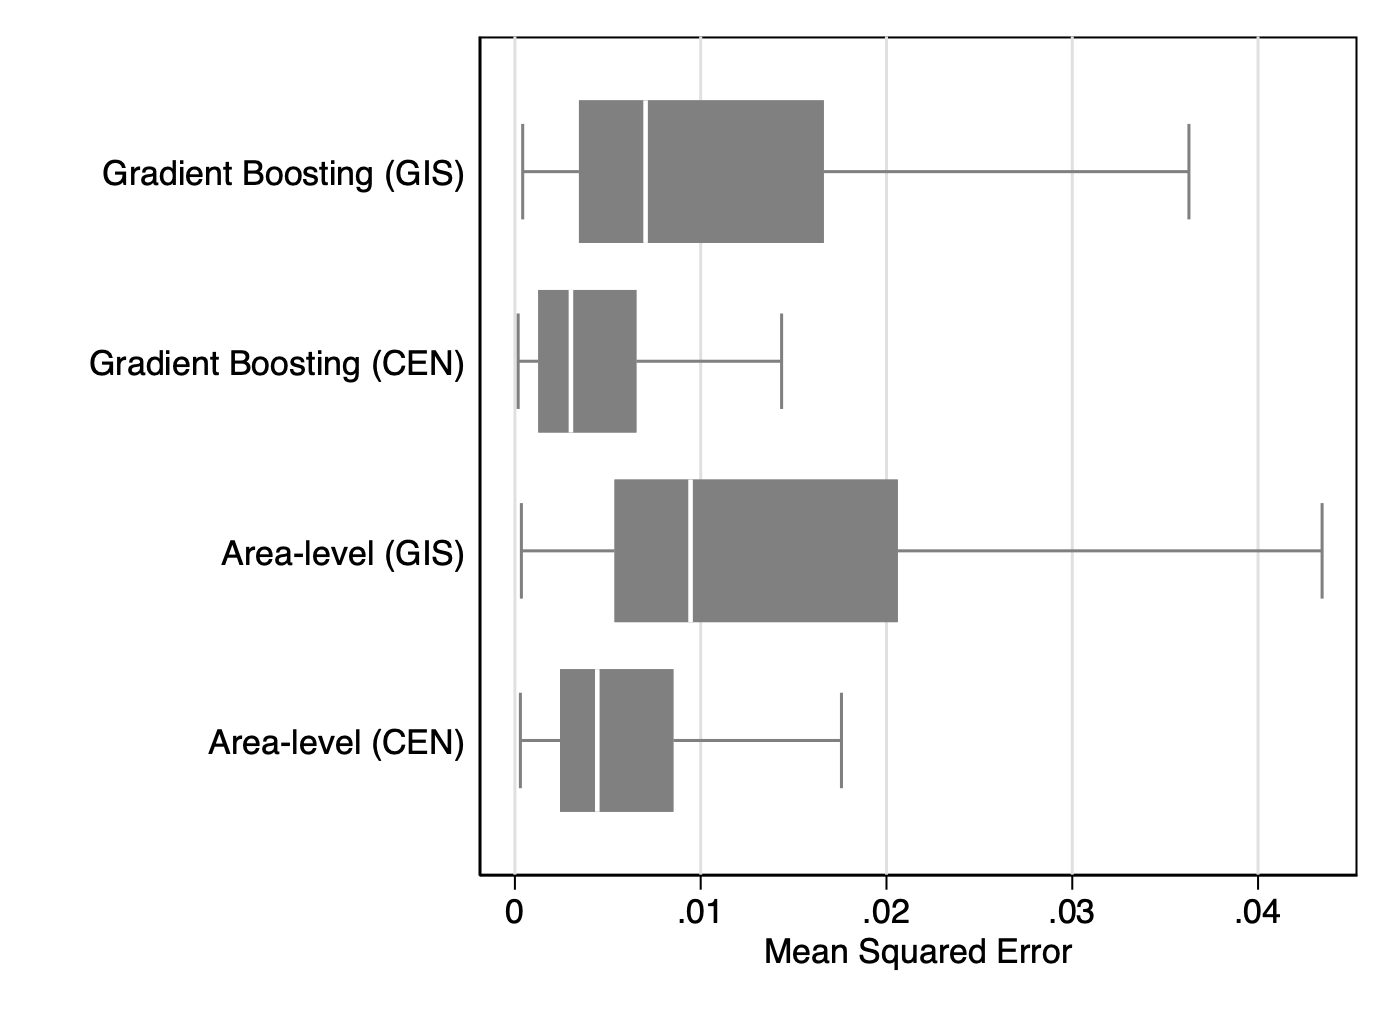
\includegraphics[scale=0.3]{Figure-3a}
\par\end{centering}
}\DIFaddFL{\hspace{0cm}}\subfloat[Targeting performance]{\begin{centering}
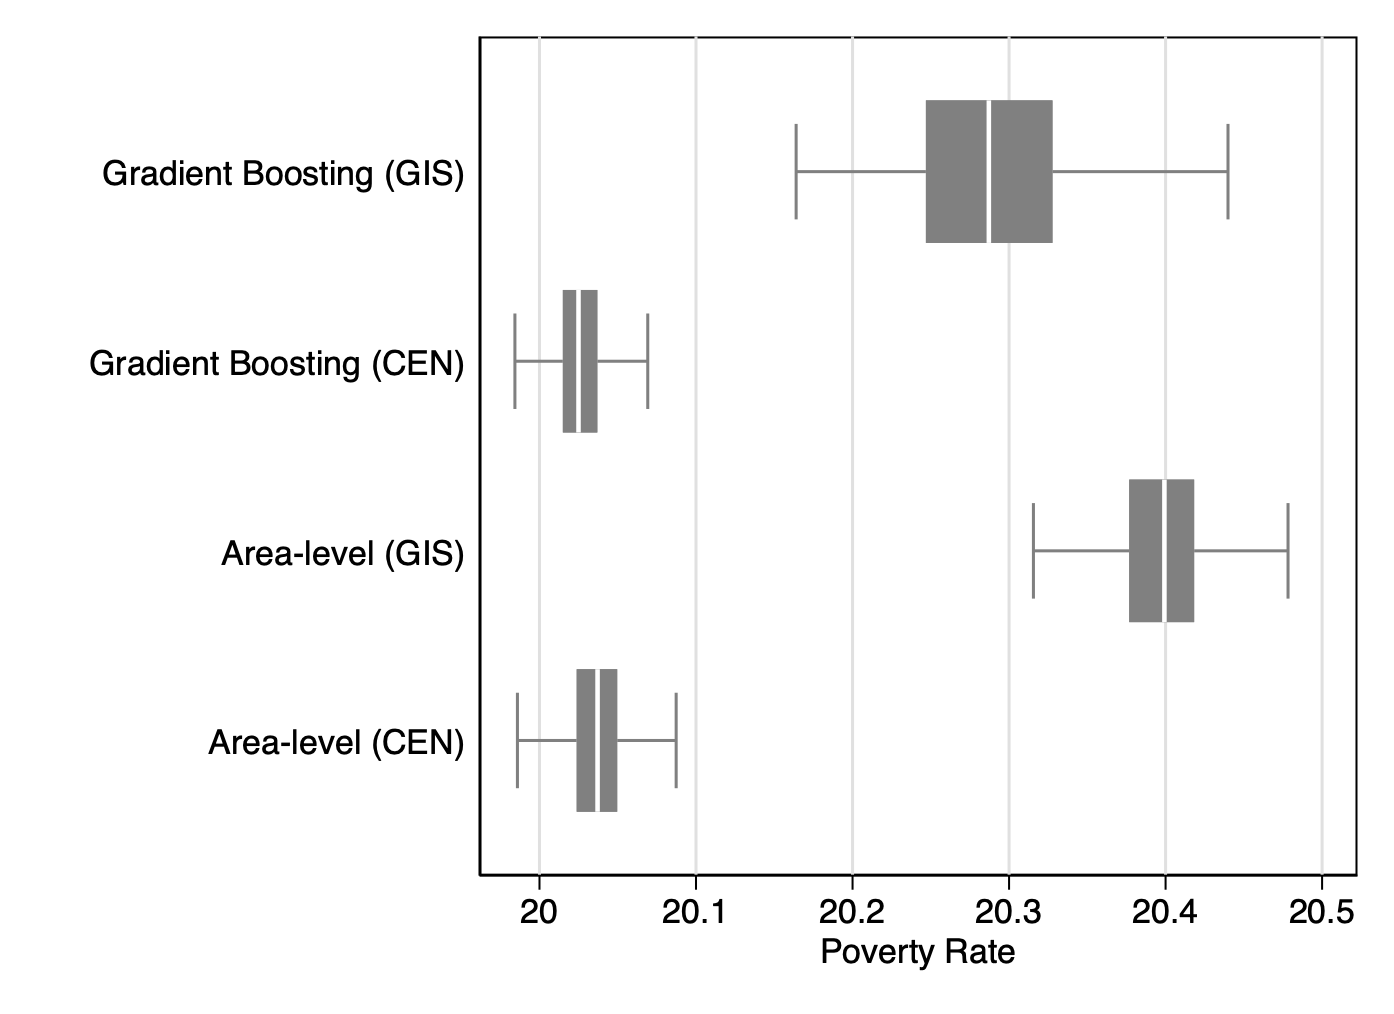
\includegraphics[scale=0.3]{Figure-3b}
\par\end{centering}
}
\DIFaddendFL \par\end{centering}
\centering{}\caption{\DIFdelbeginFL \DIFdelFL{Feature importance}\DIFdelendFL \DIFaddbeginFL \DIFaddFL{Mean squared error and targeting performance for alternative covariates
}\DIFaddendFL \protect\DIFdelbeginFL %DIFDELCMD < \label{fig:importance}%%%
\DIFdelendFL \DIFaddbeginFL \label{fig:alt_covariates}\DIFaddendFL }
\end{figure}

\DIFdelbegin \DIFdel{The performance of machine learning appears to depend heavily on the
covariates used in the model, with census-based covariates considerably
improving model performance. }\DIFdelend Another way to see that the census-based covariates have greater predictive
\DIFdelbegin \DIFdel{power }\DIFdelend \DIFaddbegin \DIFadd{capacity }\DIFaddend than the remotely-sensed covariates is by looking at feature
importance. One popular measure of feature importance summarizes the
gain (i.e., reduction of the loss function) associated with any given
feature. That is, for a given run of the model, feature importance
captures the average gain of a given feature, where the gains are
averaged across all trees in the model.\footnote{In addition, the average gains for a given run of the model are normalized
by dividing each by the sum of all average gains for that run.} Figure \DIFdelbegin \DIFdel{\ref{fig:importance} }\DIFdelend \DIFaddbegin \DIFadd{\ref{fig:feature} }\DIFaddend plots the 20 covariates with the highest
feature importance after running gradient boosting with \DIFdelbegin \DIFdel{all }\DIFdelend \DIFaddbegin \DIFadd{both census-based
(``CEN'') and remotely-sensed (``GIS'') }\DIFaddend covariates on each sample
and averaging each covariate\DIFdelbegin \DIFdel{'}\DIFdelend \DIFaddbegin \DIFadd{\textquoteright }\DIFaddend s importance across the
500 samples. We find that all of the top 10 covariates are census-based,
with only \DIFdelbegin \DIFdel{five geo-referenced }\DIFdelend \DIFaddbegin \DIFadd{six remotely-sensed }\DIFaddend covariates entering the top 20. \DIFaddbegin \DIFadd{Note
also that the feature importances outside the top 10 are relatively
small in magnitude.
}\DIFaddend 

\begin{figure}
\begin{centering}
\DIFdelbeginFL %DIFDELCMD < \subfloat[Mean squared error]{\begin{centering}
%DIFDELCMD < 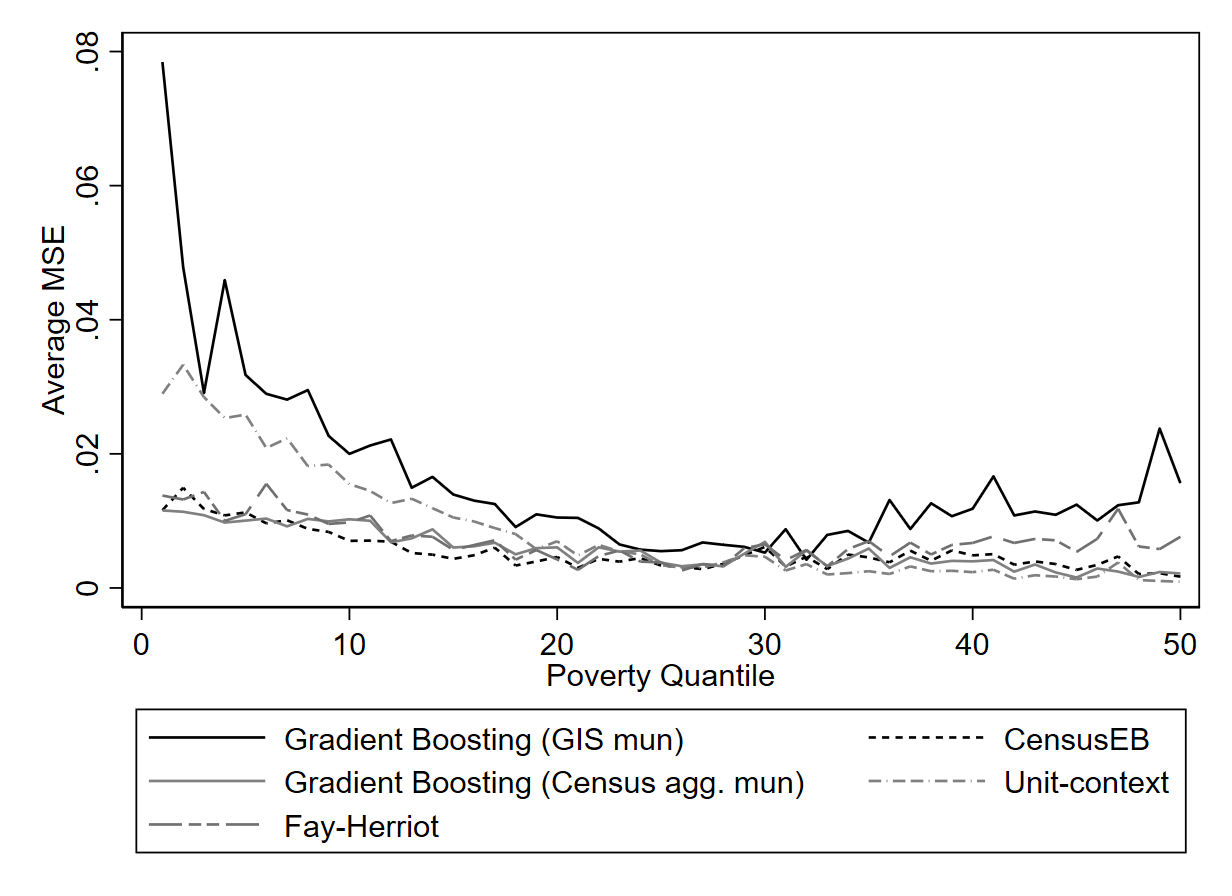
\includegraphics[scale=0.17]{Figure-4a.png}
%DIFDELCMD < \par\end{centering}
%DIFDELCMD < }%%%
\DIFdelFL{\hspace{0cm}}%DIFDELCMD < \subfloat[Bias]{\begin{centering}
%DIFDELCMD < 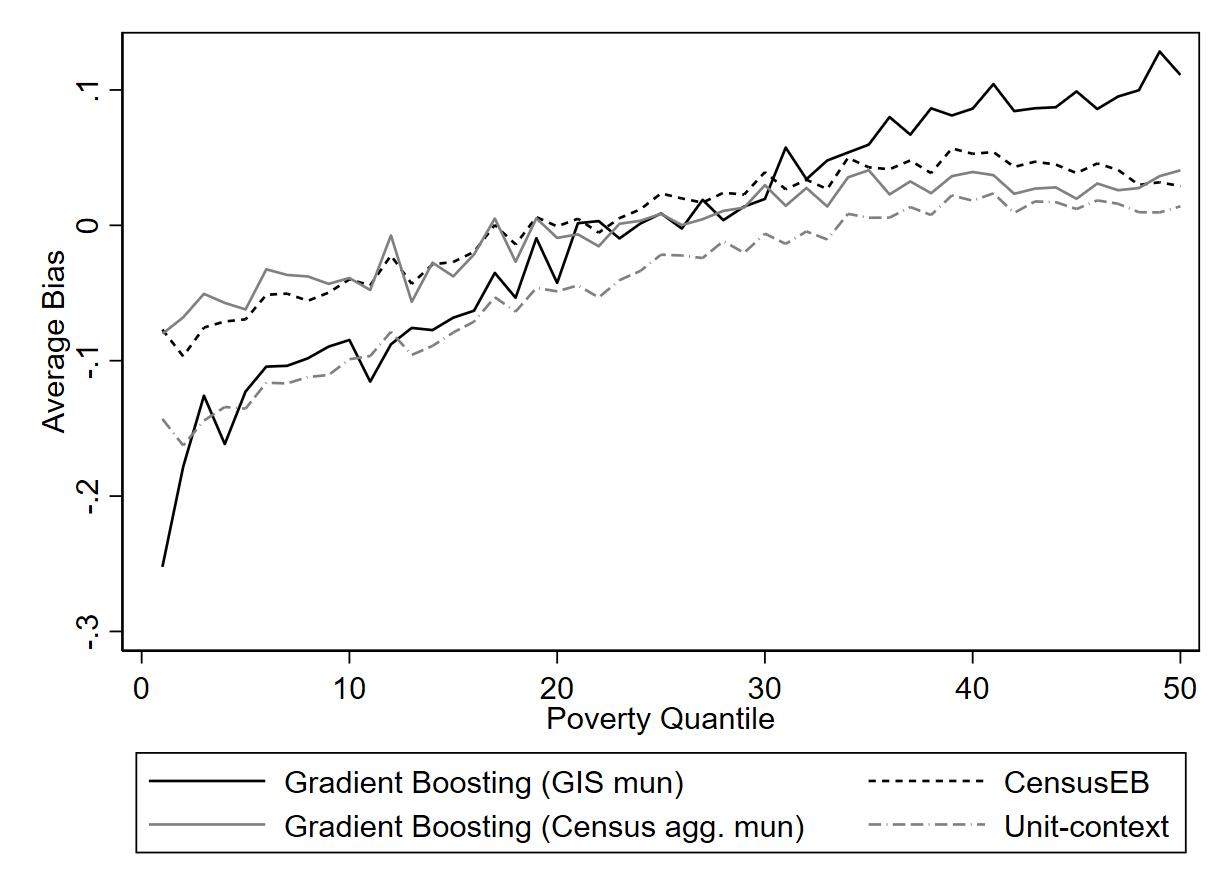
\includegraphics[scale=0.17]{Figure-4b.png}
%DIFDELCMD < \par\end{centering}
%DIFDELCMD < }
%DIFDELCMD < %%%
\DIFdelendFL \DIFaddbeginFL 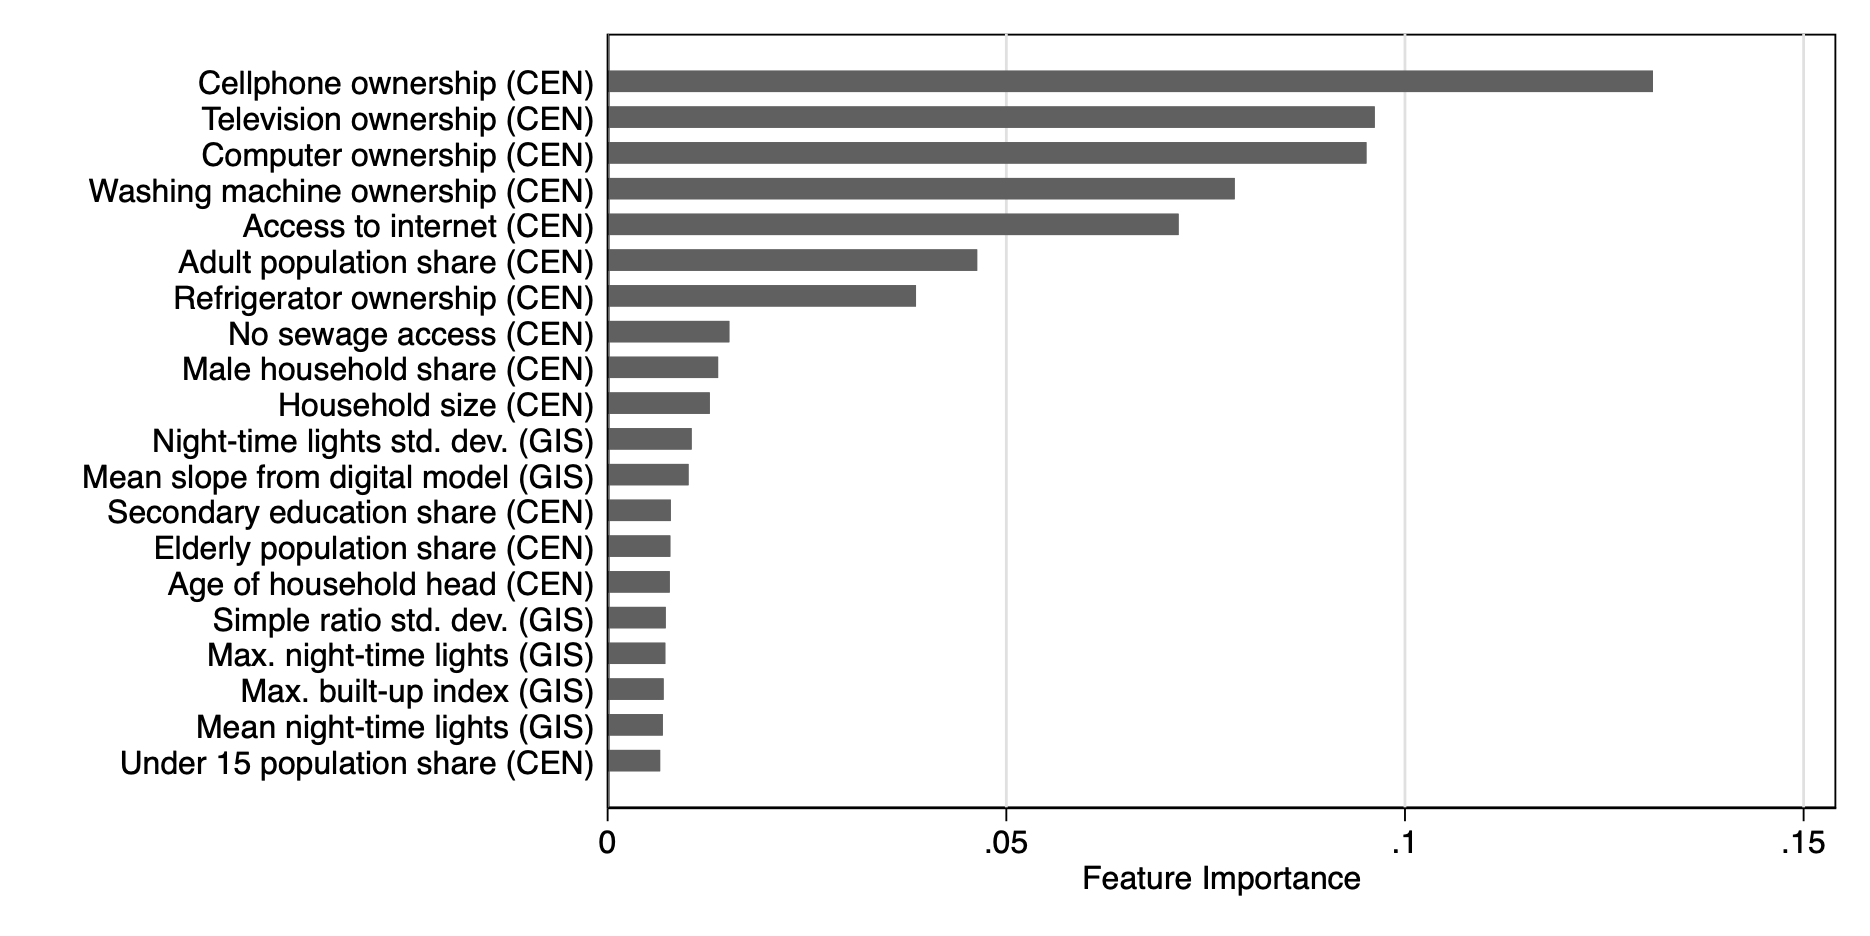
\includegraphics[scale=0.35]{Figure-4}
\DIFaddendFL \par\end{centering}
\DIFaddbeginFL \centering{}\DIFaddendFL \caption{\DIFdelbeginFL \DIFdelFL{Mean squared error and bias by poverty quantiles for select models
}\DIFdelendFL \DIFaddbeginFL \DIFaddFL{Feature importance}\DIFaddendFL \protect\DIFdelbeginFL %DIFDELCMD < \label{fig:quantiles}%%%
\DIFdelendFL \DIFaddbeginFL \label{fig:feature}\DIFaddendFL }
\end{figure}

\DIFdelbegin \DIFdel{Figure \ref{fig:quantiles} presents MSE and bias estimates for various
models across different ``poverty quantiles. '' That is, we order
all municipalities by their true poverty rates, divide them into 50
quantiles, and calculate the average MSE and bias for each quantile. For the sake of simplicity, we only present results for two machine-learning
models -- the municipality-level models using only geo-referenced
and census-based covariates -- and select traditional methods}\DIFdelend \DIFaddbegin \DIFadd{The above results suggest that gradient boosting can approximate the
performance of the unit-level model and outperform the area-level
model when using the same covariates. The aggregated nature of our
performance comparisons thus far, however, mask some important differences
between the methods. To illustrate these differences, we first use
the variance-bias decomposition presented in Eq. (\ref{eq:mseg})
and plot the two components independently}\DIFaddend . Panel (a) \DIFdelbegin \DIFdel{presents the MSE results and panel (b) presents the bias results. In both plots, gradient boosting
with census-based covariates performs
quite similarly to the ``gold standard'' unit-level model
across
all quantiles. However, }\DIFdelend \DIFaddbegin \DIFadd{of Figure \ref{fig:decomposition}
presents boxplots summarizing the distribution of the variance component
across municipalities for select models. We see that gradient boosting
is associated with lower variance estimates than the area-level model
for any given set of covariates. For example, the median variance
for }\DIFaddend gradient boosting with \DIFdelbegin \DIFdel{geo-referenced covariates again departs considerably from this benchmark, particularly at the lowest and highest quantiles. The bias results are particularly notable:
the model with geo-referenced covariates systematically underestimates
poverty at the lowest quantiles and overestimates poverty at the highest
quantiles. The standard implementation thus understates the spatial
distribution of poverty}\DIFdelend \DIFaddbegin \DIFadd{remotely-sensed covariates is 0.002 whereas
the median variance for the area-level model with the same covariates
is 0.005. This variance reduction is an important advantage of gradient
boosting and the reason for its use of regularization}\DIFaddend .

\begin{figure}
\begin{centering}
\DIFdelbeginFL %DIFDELCMD < \subfloat[Design MSE]{\begin{centering}
%DIFDELCMD < 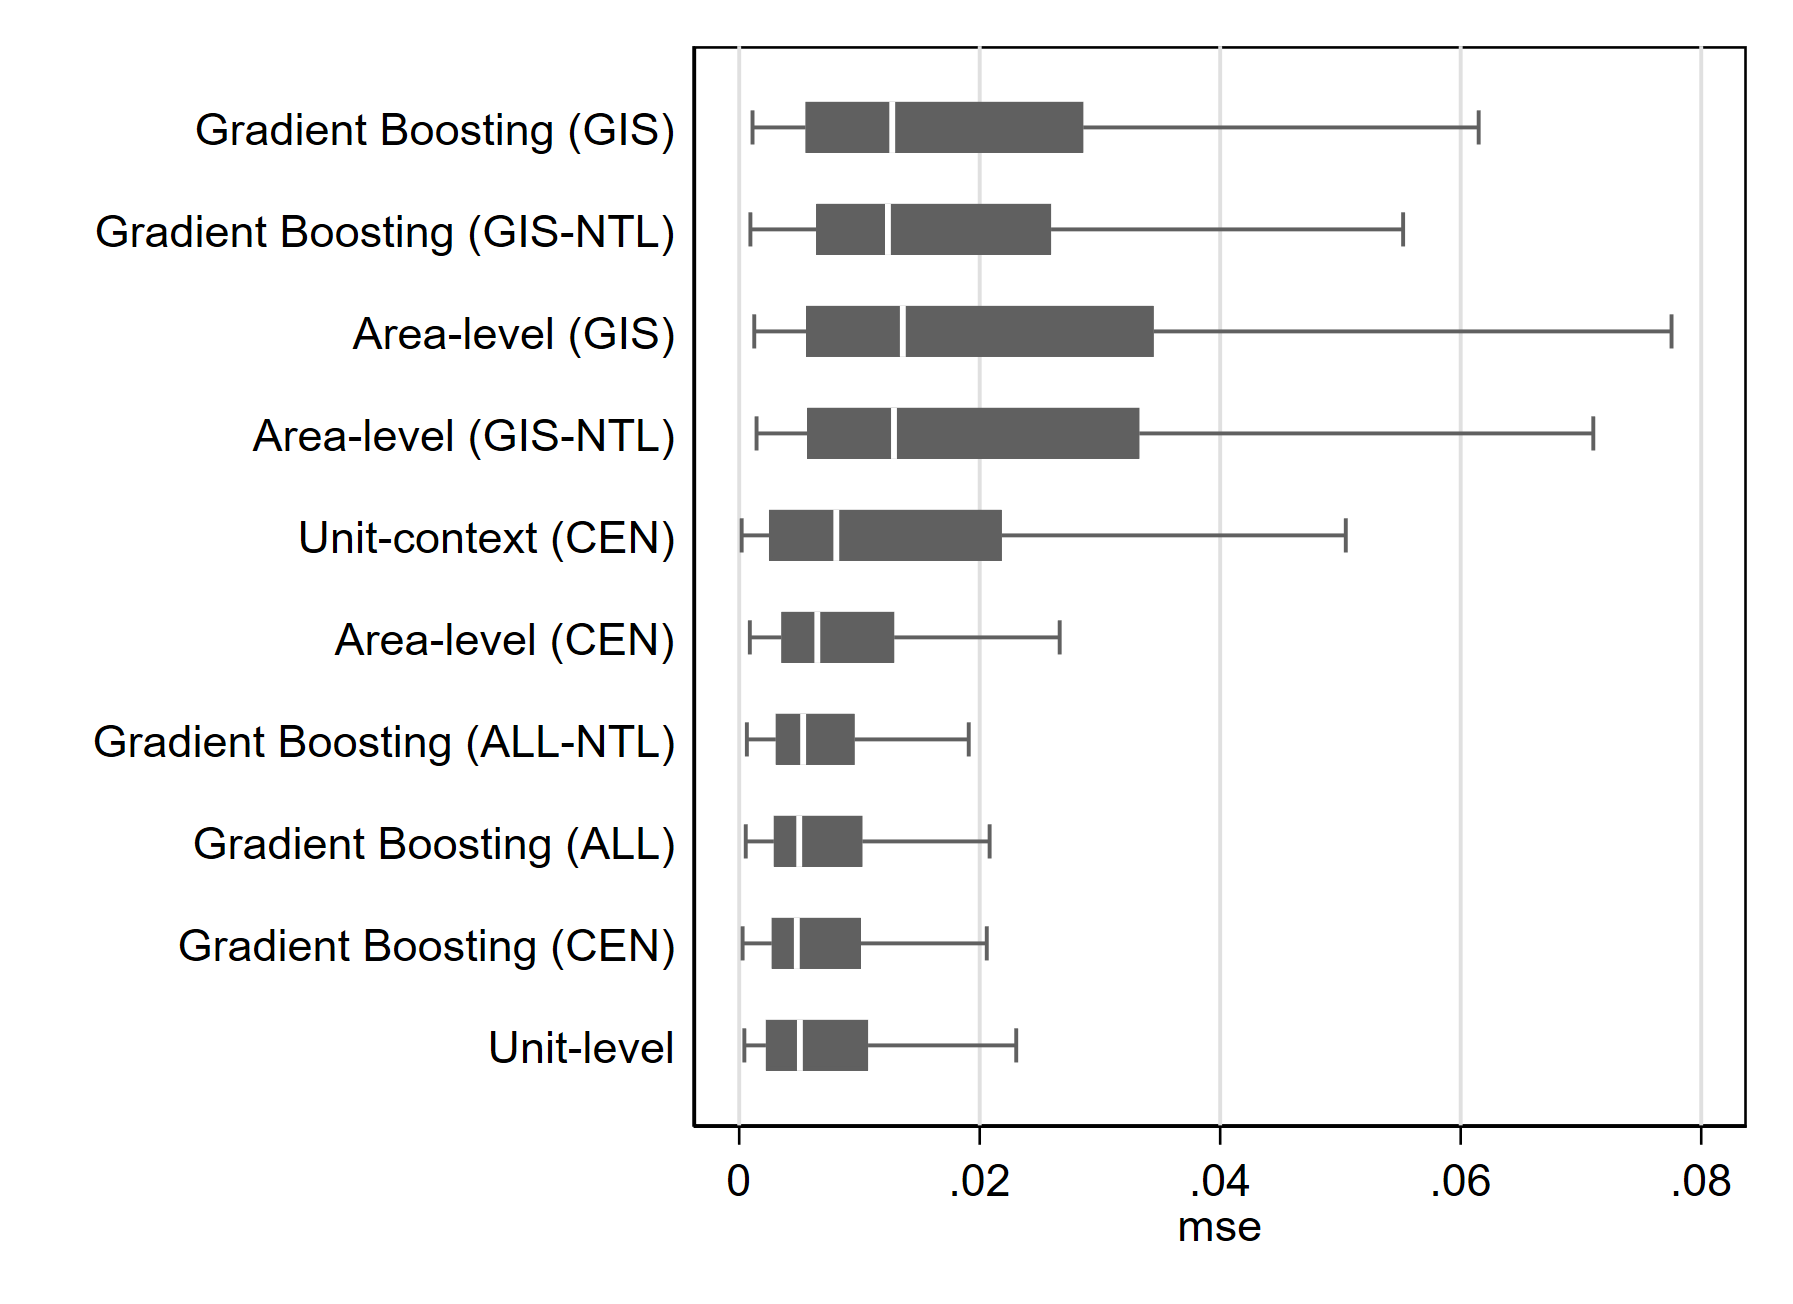
\includegraphics[scale=0.18]{Figure-3_1a.png}
%DIFDELCMD < \par\end{centering}
%DIFDELCMD < }%%%
\DIFdelFL{\hspace{0cm}}%DIFDELCMD < \subfloat[Design bias]{\begin{centering}
%DIFDELCMD < 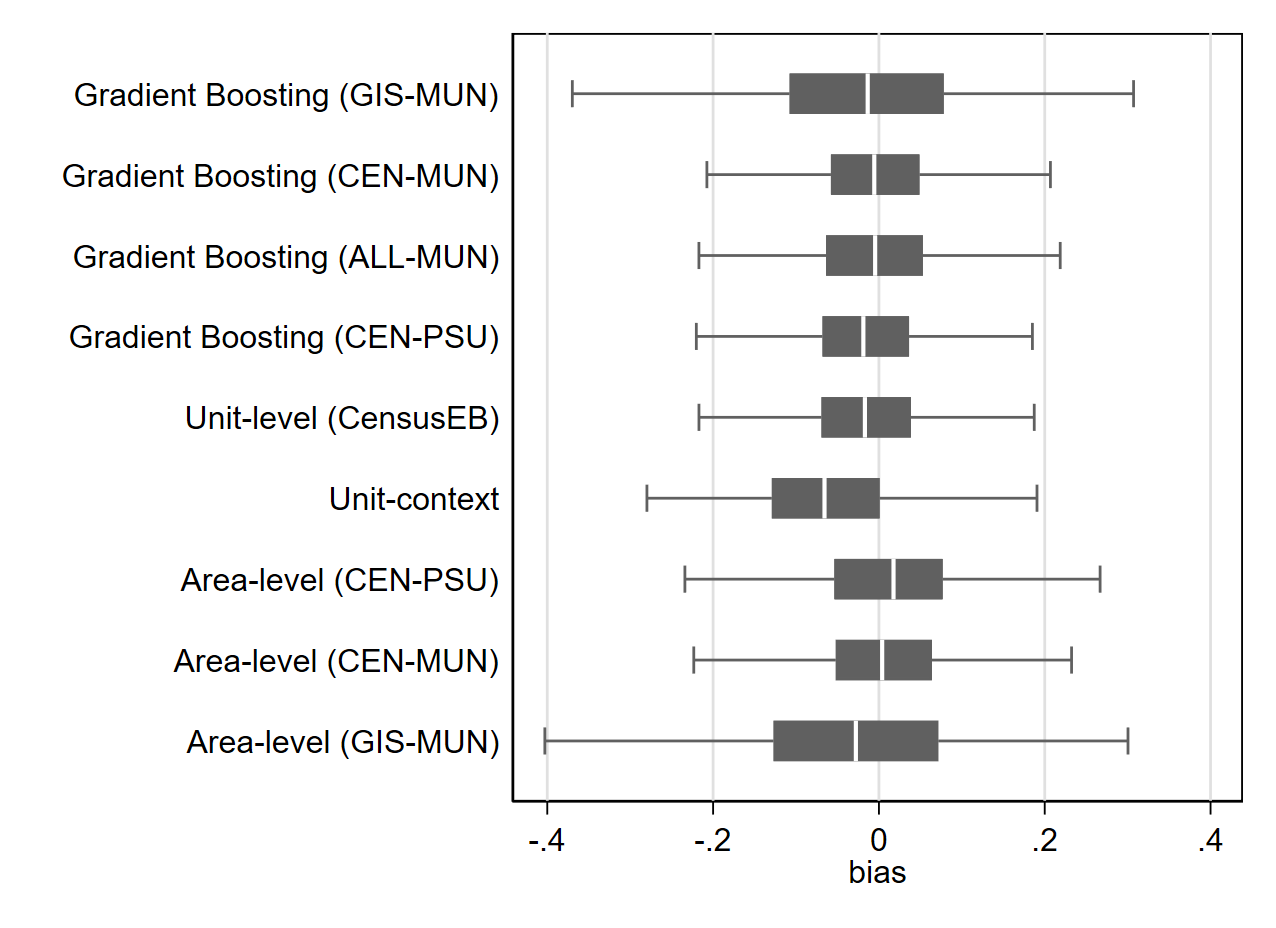
\includegraphics[scale=0.18]{Figure-3_2a.png}
%DIFDELCMD < \par\end{centering}
%DIFDELCMD < }
%DIFDELCMD < %%%
\DIFdelendFL \DIFaddbeginFL \subfloat[Variance]{\begin{centering}
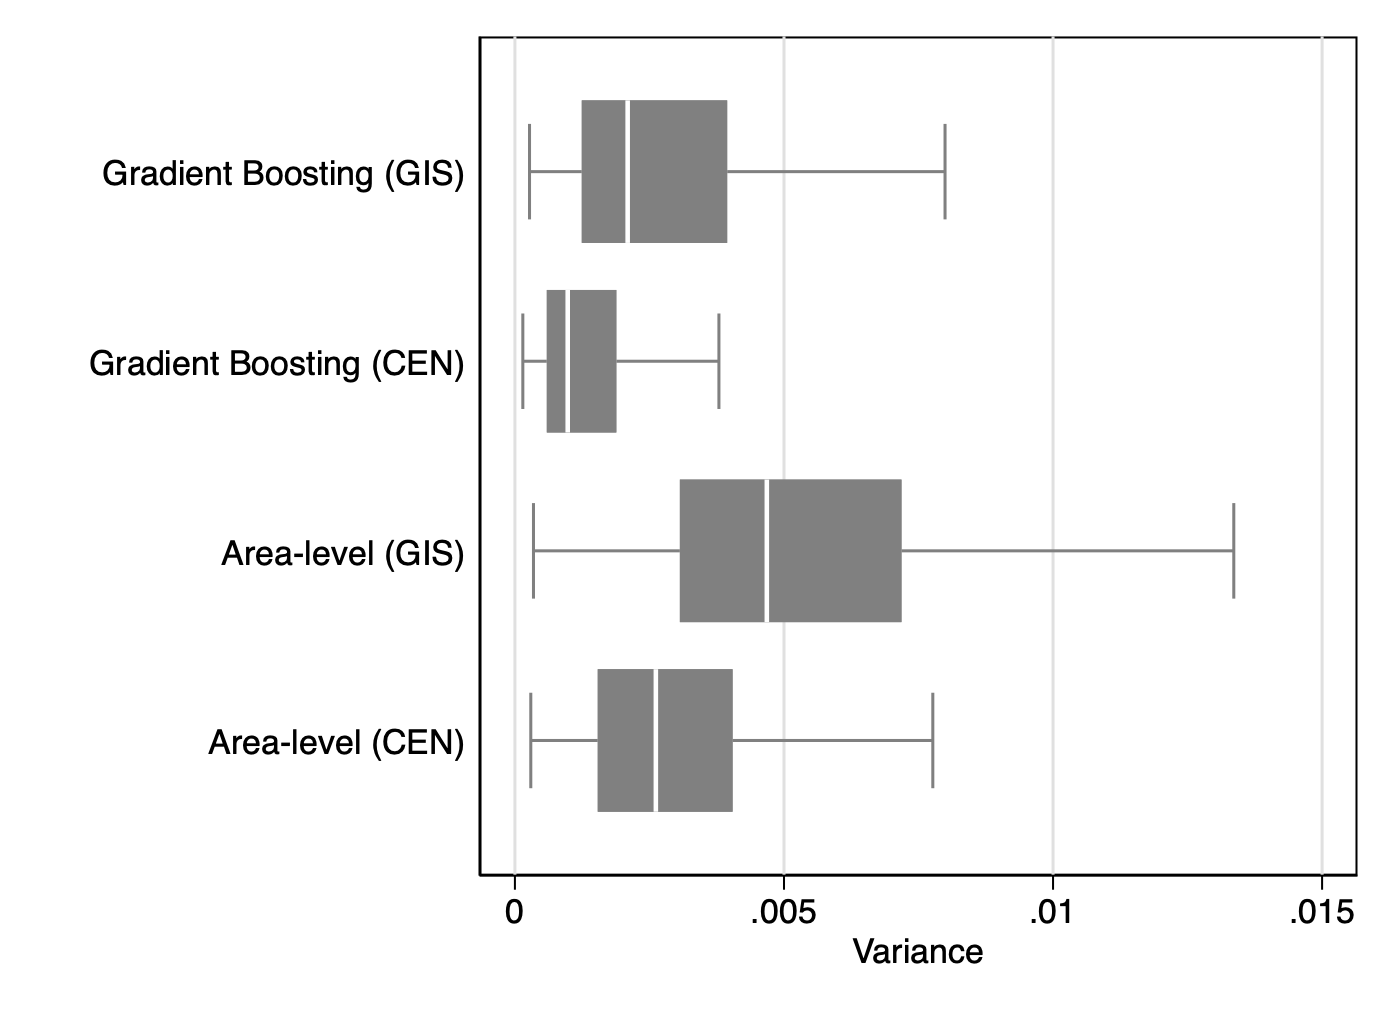
\includegraphics[scale=0.3]{Figure-5a}
\par\end{centering}
}\DIFaddFL{\hspace{0cm}}\subfloat[Bias]{\begin{centering}
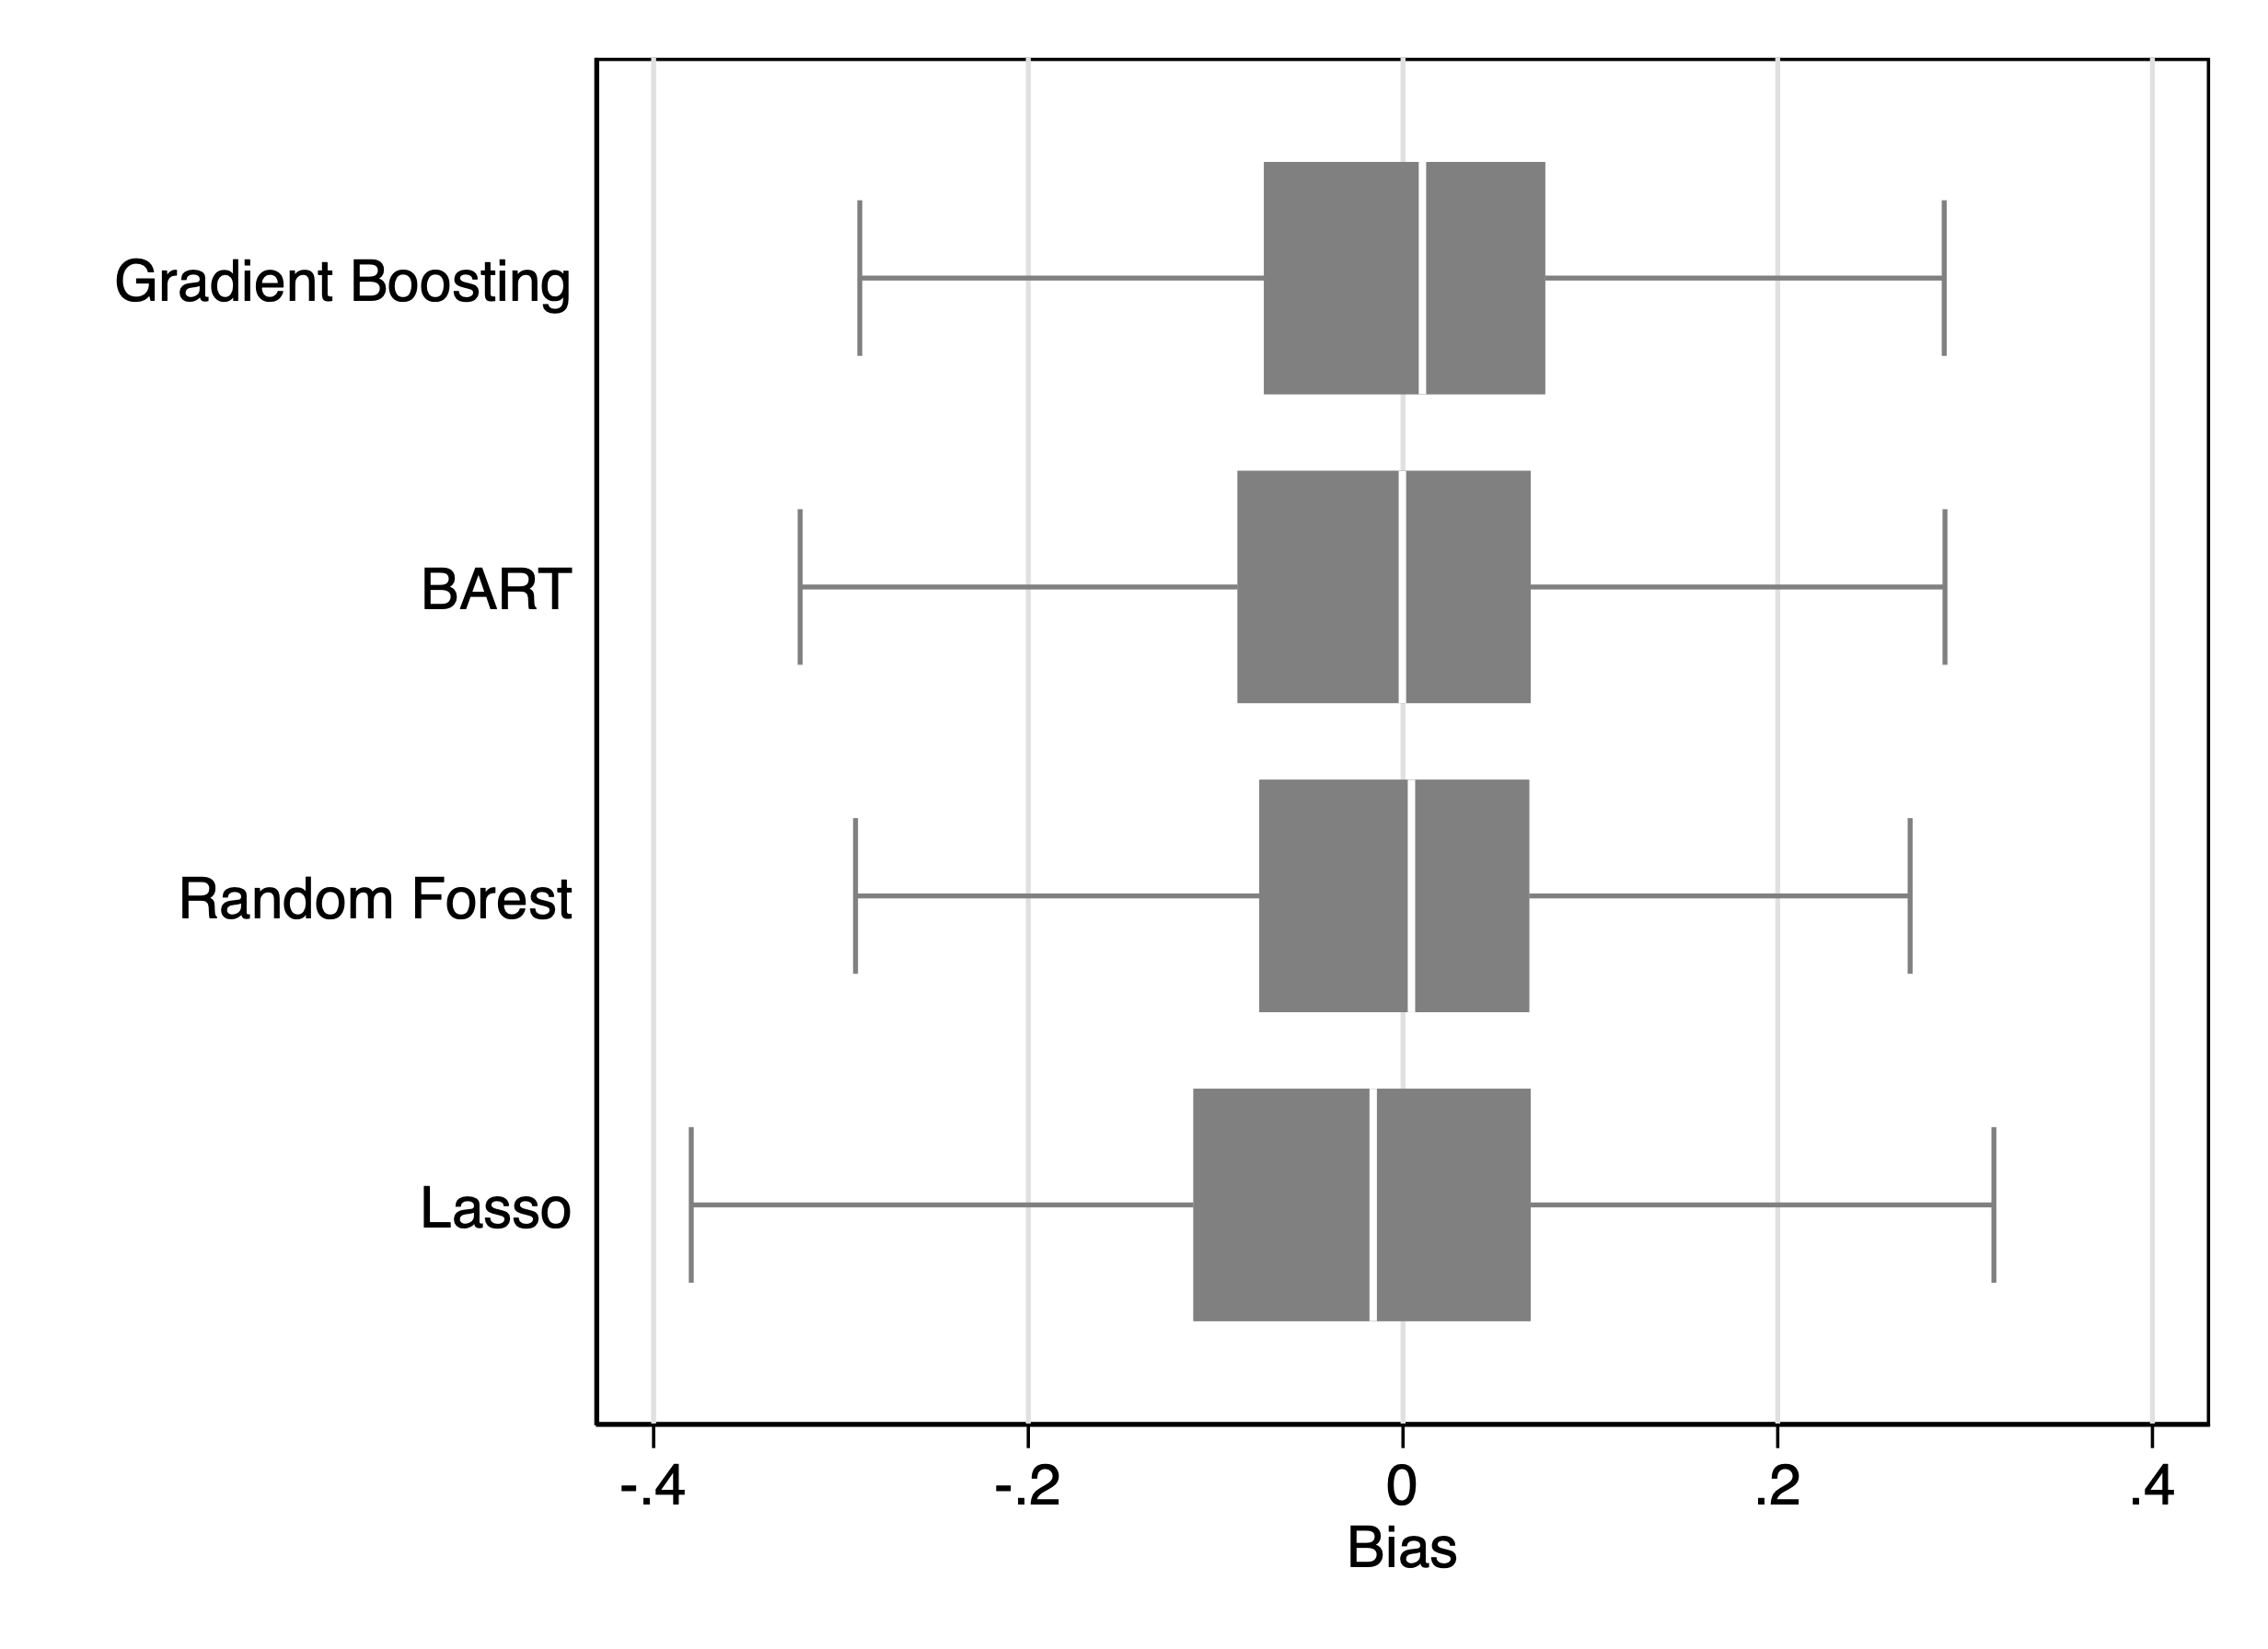
\includegraphics[scale=0.3]{Figure-5b}
\par\end{centering}
}
\DIFaddendFL \par\end{centering}
\DIFdelbeginFL %DIFDELCMD < \caption{%
{%DIFAUXCMD
\DIFdelFL{Empirical design MSE and bias with alternative machine-learning models
among 20 percent least likely to be sampled municipalities }%DIFDELCMD < \protect\label{fig:ll_sample_q1}%%%
}
%DIFAUXCMD
%DIFDELCMD < \end{figure}
%DIFDELCMD < 

%DIFDELCMD < \begin{figure}
%DIFDELCMD < %%%
%DIFDELCMD < \caption{%
{%DIFAUXCMD
\DIFdelFL{Empirical design MSE and bias with alternative machine-learning models
among 20 percent most likely to be sampled municipalities }%DIFDELCMD < \protect\label{fig:ll_sample_q5}%%%
}
%DIFAUXCMD
%DIFDELCMD < 

%DIFDELCMD < %%%
\DIFdelendFL \centering{}\DIFdelbeginFL %DIFDELCMD < \subfloat[Design MSE]{\begin{centering}
%DIFDELCMD < 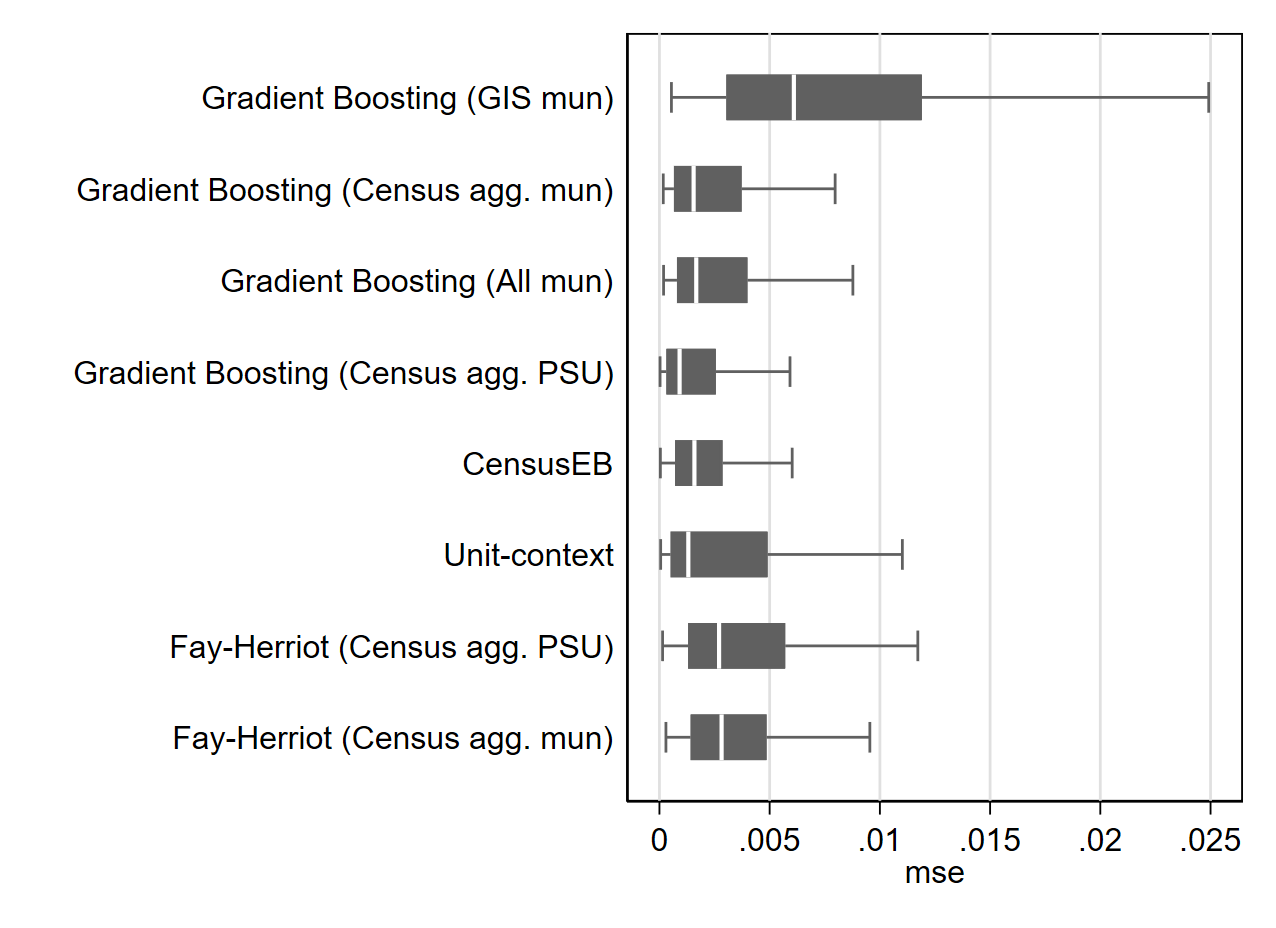
\includegraphics[scale=0.18]{Figure-3_1b.png}
%DIFDELCMD < \par\end{centering}
%DIFDELCMD < }%%%
\DIFdelFL{\hspace{0cm}}%DIFDELCMD < \subfloat[Design bias]{\begin{centering}
%DIFDELCMD < 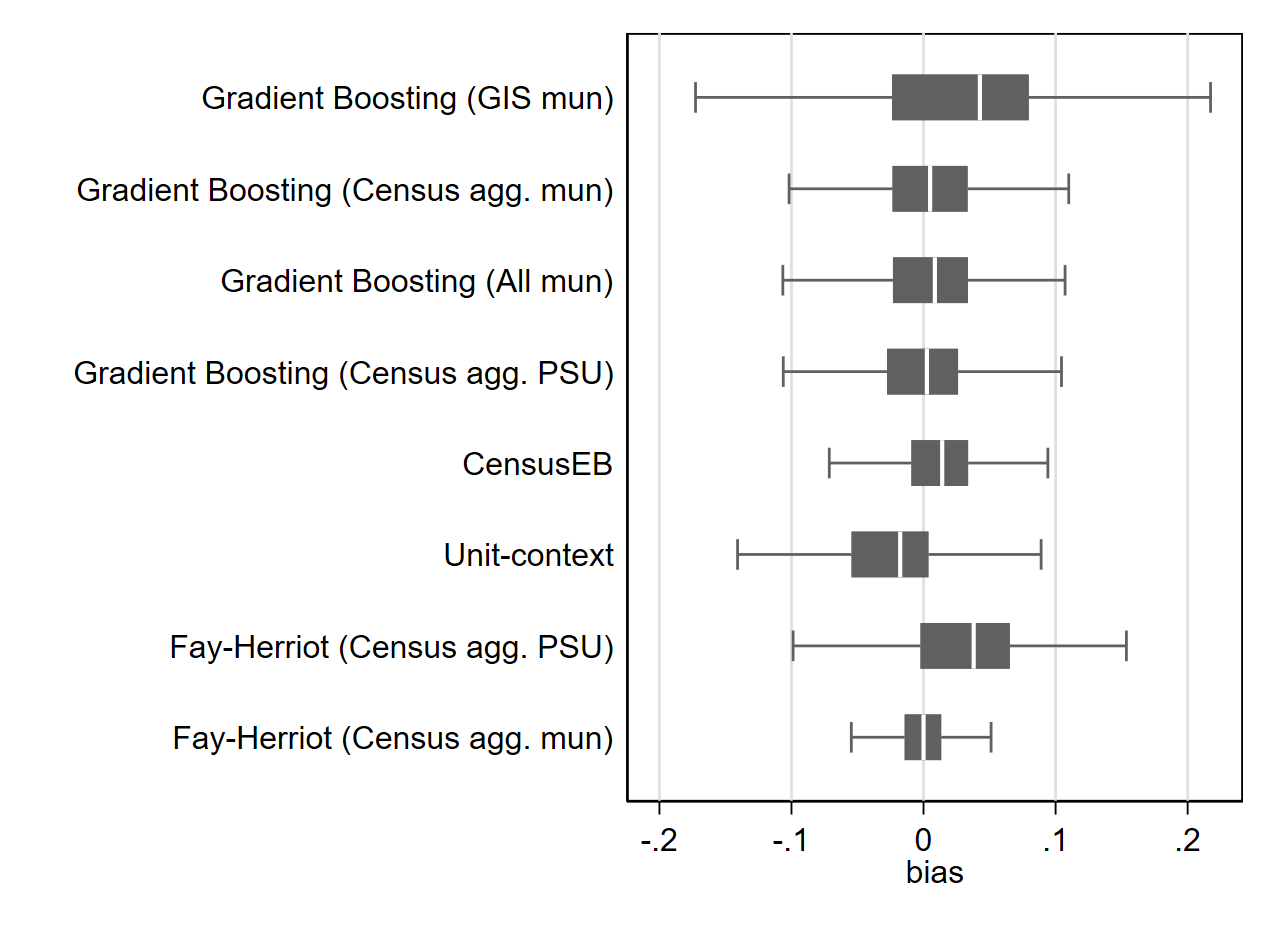
\includegraphics[scale=0.18]{Figure-3_2b.png}
%DIFDELCMD < \par\end{centering}
%DIFDELCMD < }
%DIFDELCMD < %%%
\DIFdelendFL \DIFaddbeginFL \caption{\DIFaddFL{Variance-bias decomposition for select models }\protect\label{fig:decomposition}}
\DIFaddendFL \end{figure}

\DIFdelbegin \DIFdel{An additional consideration is how the methods perform for predictions
which are out of sample. Because the experiment consists of 500 samples
taken from the
census data, a given municipality may be present in
one of the samples and may be absent in others. Consequently, to evaluate
out of sample properties we rank municipalities by their likelihood
of selection across the 500 samples. The likelihood of being present
ranges from 0.09 to 1, with a medianof 0.48 and a mean of 0.53.Among
the 20 percent least likely to be sampled municipalities, the gradient
boosting model with GIS-based covariates is the worst performing in terms of MSE followed closely by unit-context models (Figure \ref{fig:ll_sample_q1}).
In terms of bias among the 20 percent of municipalities that are least
likely to be sampled,
the gradient boosting model with
}\DIFdelend \DIFaddbegin \DIFadd{Panel (b) presents the bias component of }\DIFaddend the \DIFdelbegin \DIFdel{geo-referenced
covariates shows very wide variability, while unit context models
show downward bias.
The other gradient boosting models perform similarly
to unit-level models in terms of bias and MSE. The performance, in
terms of MSE, of the different methods seems to improve with the likelihood
of being selected. Among municipalities most likely to be selected, the gradient boosting model with the geo-referenced covariates is
still the worst performing (Figure \ref{fig:ll_sample_q5}).
However, in terms of bias, among the most likely to be selected municipalities,
the bias of Fay-Herriot methods at the municipality level is the best
performing illustrating the importance of the method's EBLUP. }\DIFdelend \DIFaddbegin \DIFadd{decomposition for the
same set of models and shows that all the models depicted are approximately
unbiased at the median.}\footnote{\DIFadd{The variance-bias decomposition shows that the MSE is the sum of the
variance and the squared bias of the estimates. To illustrate both
underestimates and overestimates, we do not square the bias estimates.}} \DIFadd{The models using remotely-sensed covariates nevertheless exhibit
wide variation in the bias estimates, implying that the estimated
poverty rates for some municipalities are severely biased. For example,
the minimum and maximum bias estimates for gradient boosting with
remotely-sensed covariates are -45 and 40 percentage points, respectively.
The area-level model exhibits similar variation in the bias estimates
when using remotely-sensed covariates, indicating that weak predictors
can produce considerable biases for both methods, at least for some
municipalities. While gradient boosting and the area-level model appear
to be similarly biased for any given covariate set, a closer look
at the source of these biases reveals an important shortcoming of
gradient boosting.
}\DIFaddend 

\DIFdelbegin %DIFDELCMD < \begin{figure}
%DIFDELCMD < \begin{centering}
%DIFDELCMD < \subfloat[Mean squared error]{\begin{centering}
%DIFDELCMD < 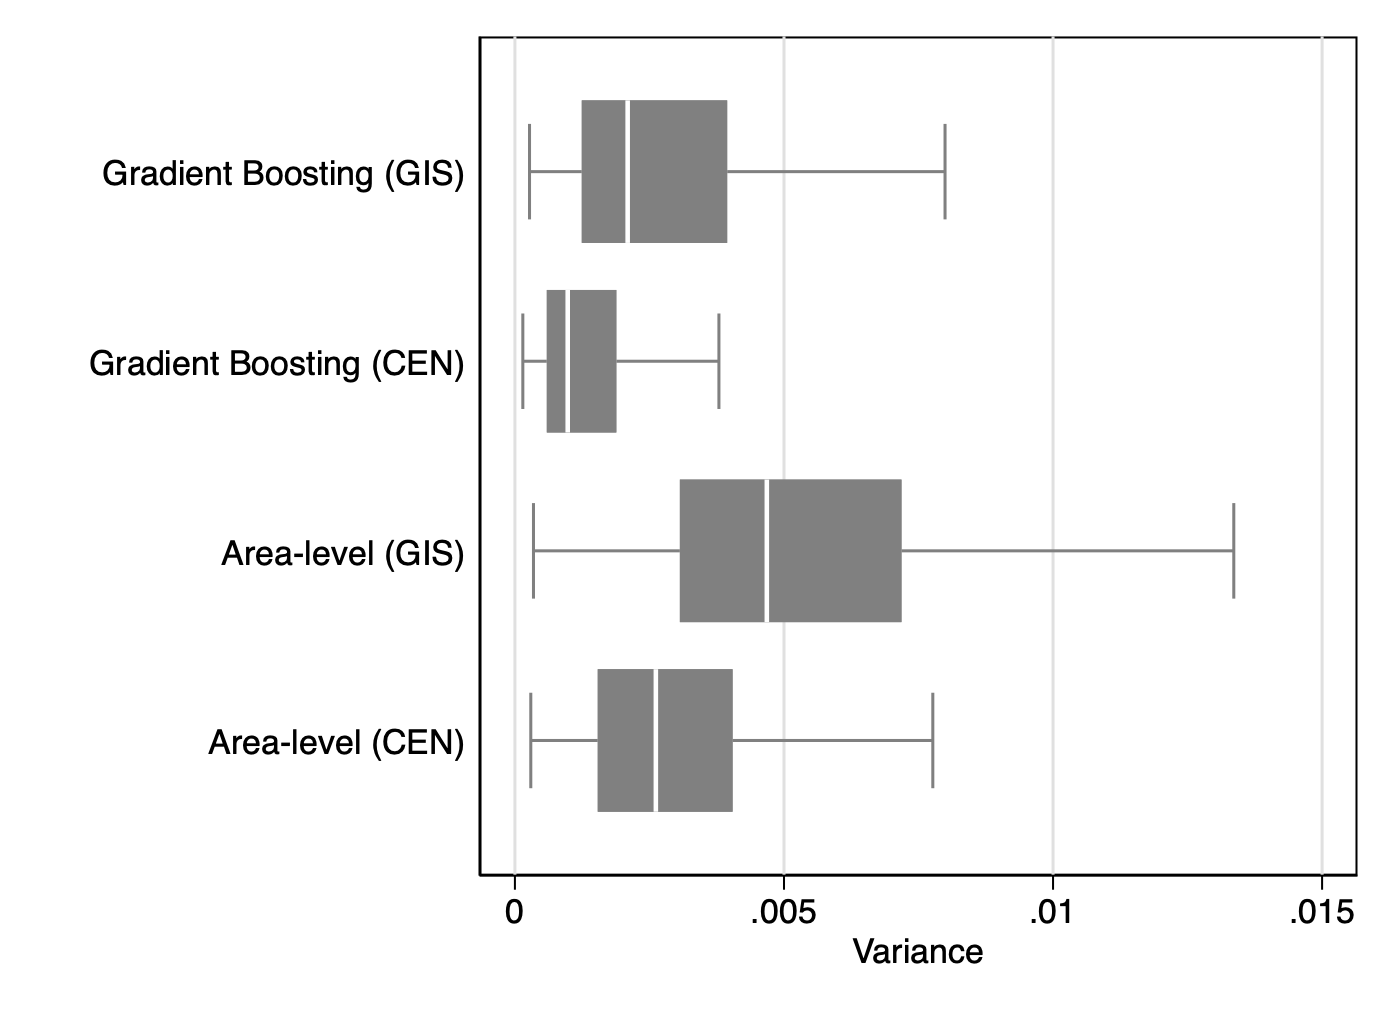
\includegraphics[scale=0.17]{Figure-5a}
%DIFDELCMD < \par\end{centering}
%DIFDELCMD < 

%DIFDELCMD < }%%%
\DIFdelFL{\hspace{0cm}}%DIFDELCMD < \subfloat[Bias]{\begin{centering}
%DIFDELCMD < 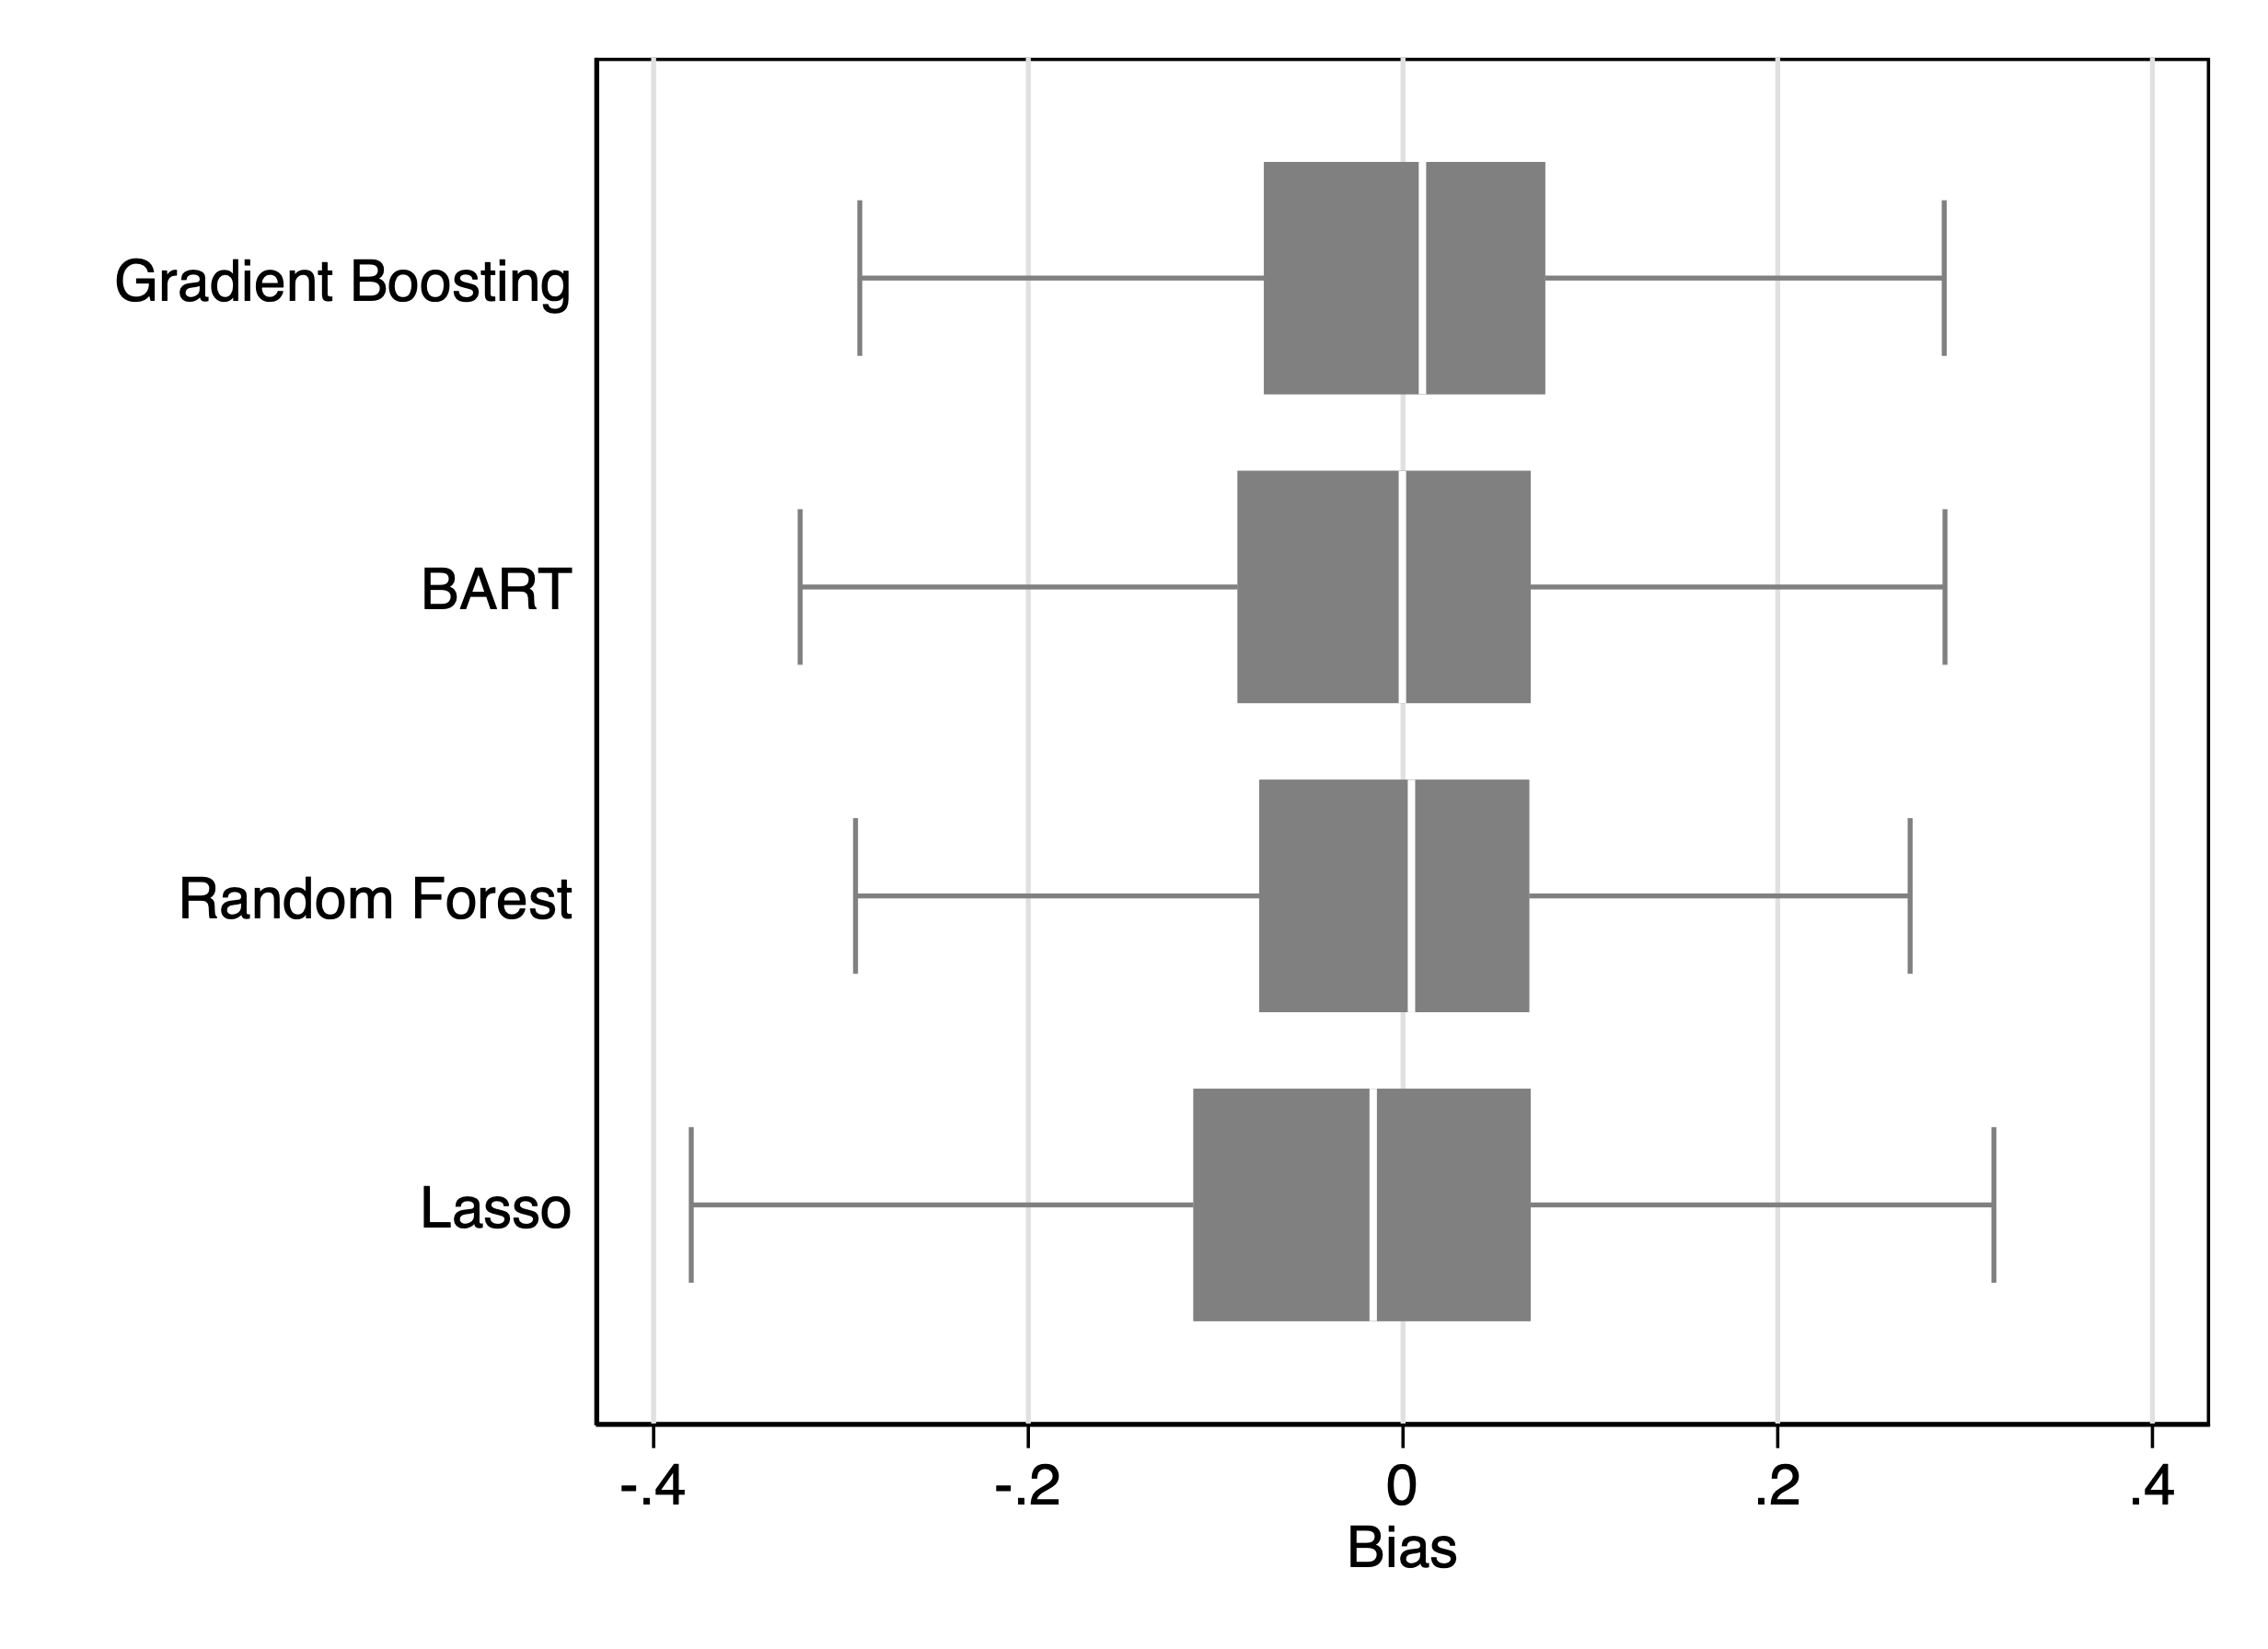
\includegraphics[scale=0.17]{Figure-5b}
%DIFDELCMD < \par\end{centering}
%DIFDELCMD < 

%DIFDELCMD < }
%DIFDELCMD < \par\end{centering}
%DIFDELCMD < %%%
%DIFDELCMD < \caption{%
{%DIFAUXCMD
\DIFdelFL{Mean squared error and bias for alternative machine learning models
}%DIFDELCMD < \protect\label{fig:ml}%%%
}
%DIFAUXCMD
%DIFDELCMD < \end{figure}
%DIFDELCMD < 

%DIFDELCMD < %%%
\DIFdel{While we have focused on the performance of gradient boosting up to
this point, there are nevertheless several other machine-learning
models that can be used for poverty mapping. Leading alternatives
include the least absolute shrinkage and selection operator (lasso)
\mbox{%DIFAUXCMD
\citep{tibshirani1996}}\hskip0pt%DIFAUXCMD
, the random forest \mbox{%DIFAUXCMD
\citep{breiman2001}}\hskip0pt%DIFAUXCMD
, and
Bayesian additive regression trees (BART) \mbox{%DIFAUXCMD
\citep{chipman2010bart}}\hskip0pt%DIFAUXCMD
. While the lasso is a simple way to conduct variable selection and
regularization in the context of linear regression, the random forest
and BART models are similar to gradient boosting in that they all
rely on regression tree frameworks. We ask whether these alternative
models can perform better than gradient boosting within the confines
of the standard implementation, which relies exclusively on }\DIFdelend \DIFaddbegin \DIFadd{To this end, panel (a) of Figure \ref{fig:poverty_sampling} plots
the municipality-level bias estimates from select models on the true
municipality poverty rates. For each model, we fit a lowess curve
to the data to show the (weighted) average of the bias estimates at
different true poverty rates. The figure shows the source of the aforementioned
bias variability: both models with }\DIFaddend remotely-sensed \DIFdelbegin \DIFdel{covariates. Panels (a) and (b) of Figure \ref{fig:ml} present the MSE and bias results for all models. With the possible exception of the lasso,
we find that all models perform comparably, meaning that
the performance of gradient boosting when using geo-referenced covariates
cannot be remedied by simply adopting a different machine-learning
model }\DIFdelend \DIFaddbegin \DIFadd{covariates severely
overestimate poverty in the least poor municipalities and underestimate
poverty in the most poor municipalities. Stated differently, the models
with remotely-sensed covariates understate the spatial distribution
of poverty. This result occurs because the predictions collapse toward
the mean in the absence of informative covariates, which produces
predictable biases in the tails of the distribution. Interestingly,
for both covariate types, the area-level model is less biased for
the poorest municipalities}\DIFaddend .

\begin{figure}
\begin{centering}
\DIFdelbeginFL %DIFDELCMD < 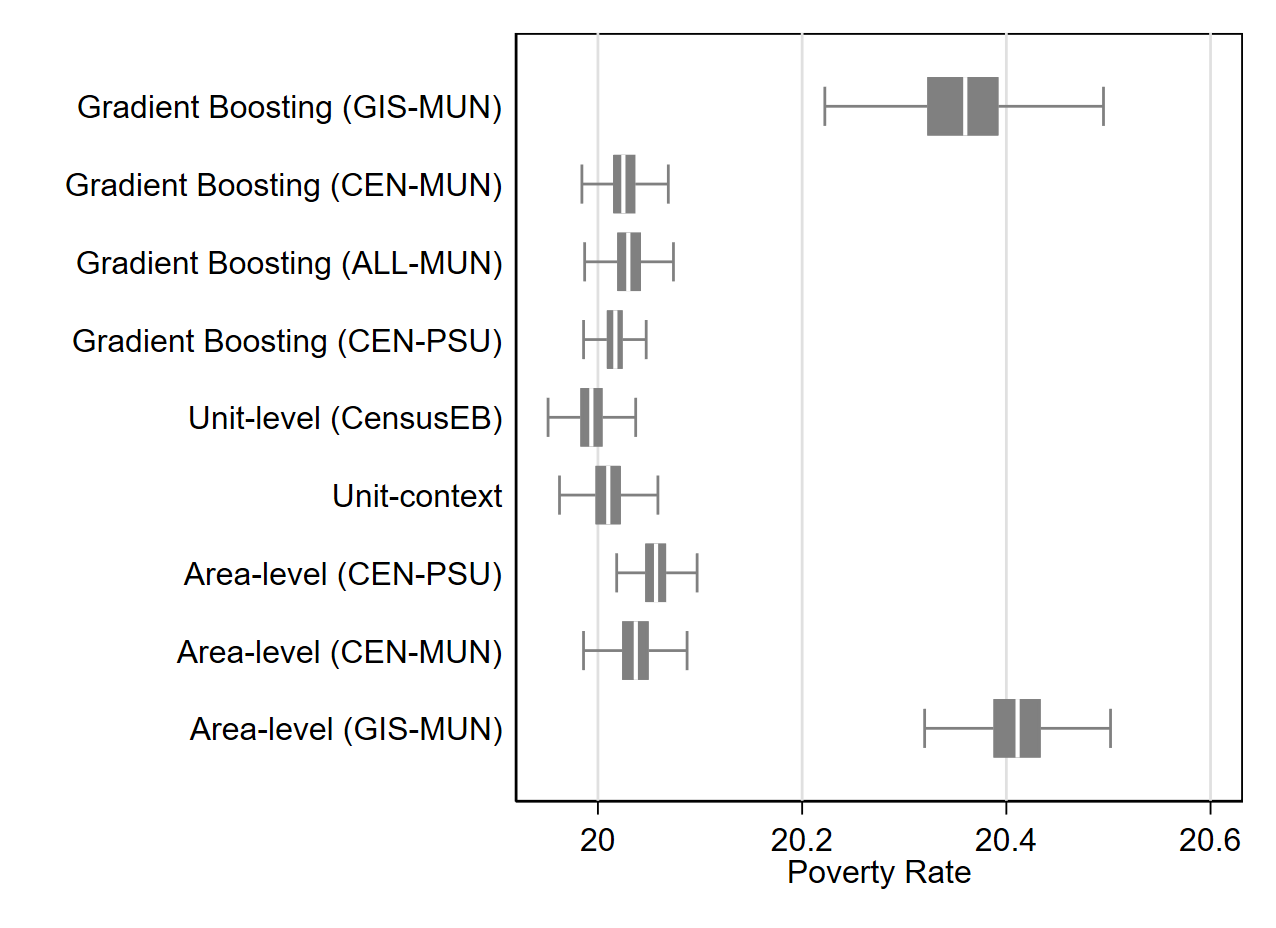
\includegraphics[scale=0.25]{Figure-6.png}
%DIFDELCMD < %%%
\DIFdelendFL \DIFaddbeginFL \subfloat[Bias by poverty rate]{\begin{centering}
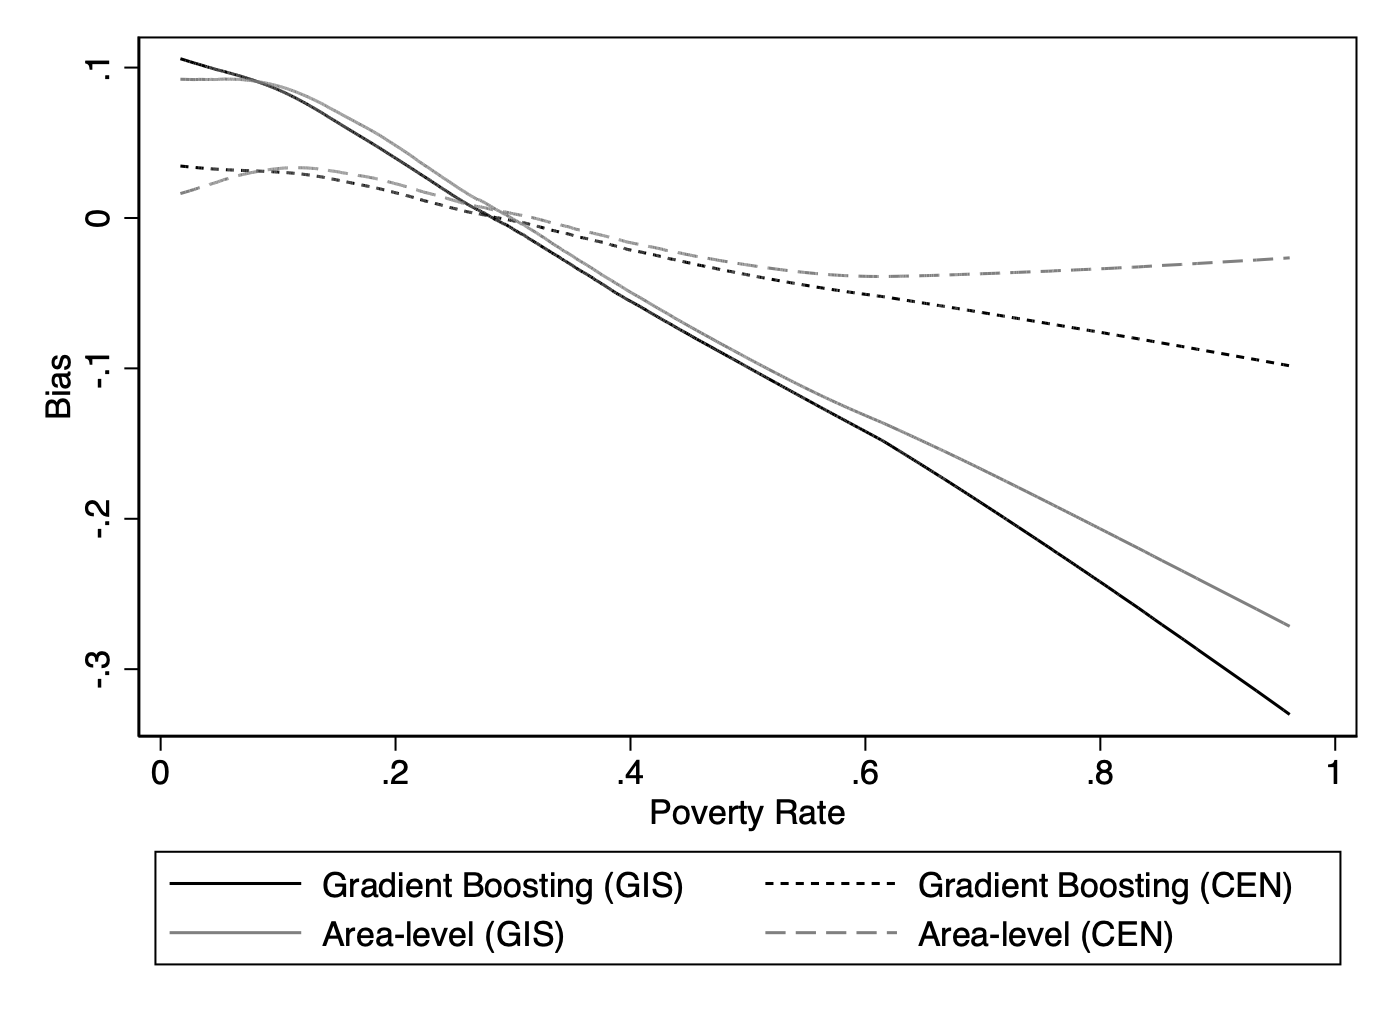
\includegraphics[scale=0.3]{Figure-6a}
\par\end{centering}
}\DIFaddFL{\hspace{0cm}}\subfloat[Bias by sampling frequency]{\begin{centering}
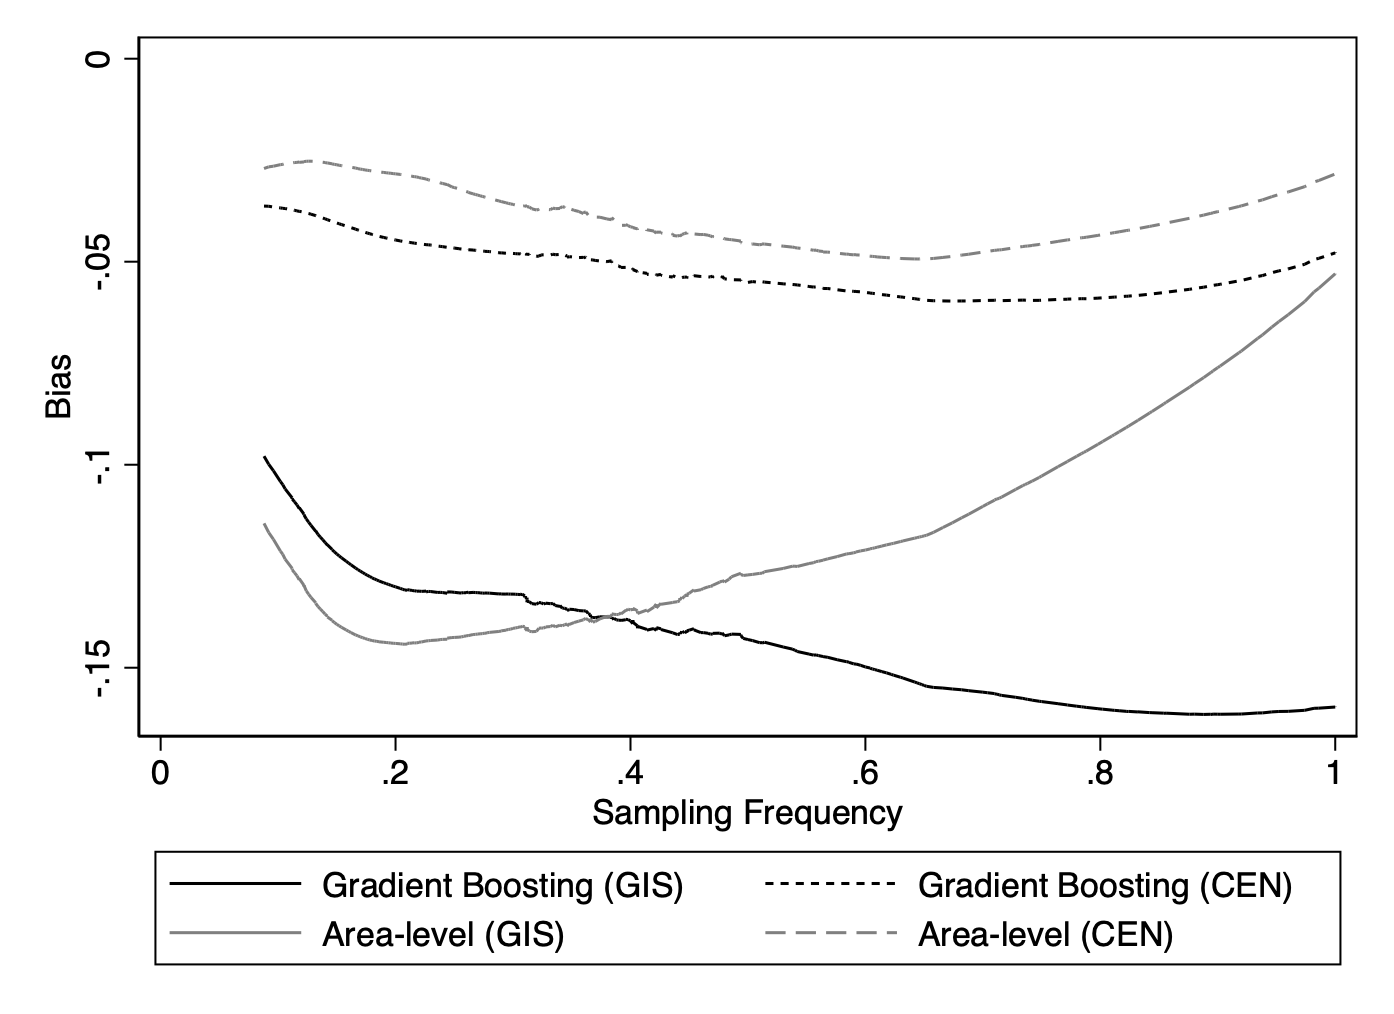
\includegraphics[scale=0.3]{Figure-6b}
\par\end{centering}
}
\DIFaddendFL \par\end{centering}
\DIFaddbeginFL \centering{}\DIFaddendFL \caption{\DIFdelbeginFL \DIFdelFL{Poverty targeting }\DIFdelendFL \DIFaddbeginFL \DIFaddFL{Bias by poverty rate and sampling frequency}\DIFaddendFL \protect\DIFdelbeginFL %DIFDELCMD < \label{fig:targeting}%%%
\DIFdelendFL \DIFaddbeginFL \label{fig:poverty_sampling}\DIFaddendFL }
\end{figure}

\DIFdelbegin \DIFdel{Finally, recall from Section \ref{sec:validation} that we argued
that the ultimate concern with poverty mapping is to understand how
different methodological choices affect poverty alleviation. Figure
\ref{fig:targeting} thus compares the machine-learning and
traditional
approaches in terms of their ability to reduce poverty in the context
of our targeting simulations.In these simulations, which is dependent
just on the povertyu ranking, a hypothetical poverty-alleviation program
targeted on the basis of }\textit{\DIFdel{true}} %DIFAUXCMD
\DIFdel{municipality-level poverty
rates is able to reduce the overall poverty headcount to just under
}\DIFdelend \DIFaddbegin \DIFadd{Panel (b) in Figure \ref{fig:poverty_sampling} shows that an important
reason for the area-level model's reduced bias is that its in-sample
predictions are a weighted average of the model-based estimates and
the (unbiased) direct estimates.}\footnote{\DIFadd{See Section \ref{sec:methods} for details. By contrast, gradient
boosting relies exclusively on the model-based estimates and only
incorporates the direct estimates when fitting the model.}} \DIFadd{For each model depicted, we focus on the }\DIFaddend 20 \DIFdelbegin \DIFdel{percent,
a 5 percentage point improvement. While the achieved poverty
rates of all models fall within the 20 percent range, we find that gradient boosting with geo-referenced covariates is one of the worst
performing models
. With the exception of the }\DIFdelend \DIFaddbegin \DIFadd{percent of municipalities
with the lowest true poverty rate, plot the municipality-level bias
estimates on the frequency with which a municipality was sampled,
and then fit a lowess curve to the data. The sampling frequencies
capture the proportion of samples for which a municipality received
an in-sample prediction, thus benefitting from the }\DIFaddend area-level \DIFdelbegin \DIFdel{model using
geo-referenced covariates, }\DIFdelend \DIFaddbegin \DIFadd{model's
averaging procedure. As expected, we see that }\DIFaddend the \DIFdelbegin \DIFdel{standard gradient boosting implementation
relying on geospatial covariates is thus outperformed by all traditional methods, including those that are direct competitors. However, when
incorporating census-based covariates, we find that gradient boosting
achieves poverty rates that are comparable to the }\DIFdelend \DIFaddbegin \DIFadd{area-level model
is less biased for municipalities with higher sampling frequencies.
The performance disparity is especially pronounced among the models
with remotely-sensed covariates, as the area-level model is roughly
10 percentage points less biased at the highest sampling frequencies.
}

\DIFadd{These latter results highlight an important methodological difference
between the modern and traditional approaches. In particular, the
machine-learning methods used for poverty mapping were developed for
out-of-sample prediction and ignore the direct estimates after fitting
the model. The }\DIFaddend traditional methods, \DIFdelbegin \DIFdel{yet again showing that an exclusive reliance on remotely-sensed data
can limit the performance of the machine learning. }%DIFDELCMD < 

%DIFDELCMD < %%%
\DIFdel{The results of the targeting simulation are relevant to cases where
targeting is based solely on the ranking of municipalities -- all
methods appear to do a solid job. Nevertheless, there are many instances
where the targeting mechanism may rely on the method's poverty estimates
}\DIFdelend \DIFaddbegin \DIFadd{by contrast, were developed specifically
for poverty mapping and recognize that mapping is partly an in-sample
prediction problem. The traditional methods thus use the direct estimates
after fitting the model and weight them more heavily when the covariates
are less informative. Interestingly, this highlights another concern
with using direct estimates to assess model performance: traditional
methods are designed to be less predictive of direct estimates when
the model is more informative. The main point here is nevertheless
that our results are in line with the expectation that traditional
methods will exhibit less in-sample bias, particularly in the presence
of weak covariates}\DIFaddend .
\DIFdelbegin \DIFdel{For example, Senegal's Unique National Registry (RNU - in French)
of vulnerable households relies on actual estimates from poverty maps
to determine the quotas for sampling by municipality (Ferre \mbox{%DIFAUXCMD
\citeyear{ferresenegal}}\hskip0pt%DIFAUXCMD
). It is in those cases where a method that yields unbiased and precise
estimates should be employed.
}\DIFdelend 

\section{Conclusion\protect\label{sec:conclusion}}

Machine-learning approaches to poverty mapping have \DIFdelbegin \DIFdel{gained considerable
popularity }\DIFdelend \DIFaddbegin \DIFadd{become increasingly
popular }\DIFaddend in recent years. In contrast to traditional \DIFdelbegin \DIFdel{poverty }\DIFdelend mapping procedures,
modern machine-learning methods rely on non-parametric statistical
techniques applied to remotely-sensed data, such as satellite imagery
or call detail records. In addition, machine-learning approaches \DIFdelbegin \DIFdel{generally }\DIFdelend \DIFaddbegin \DIFadd{routinely
}\DIFaddend conduct model assessment using the \DIFdelbegin \DIFdel{coefficient of determination
(}\DIFdelend $R^{2}$\DIFdelbegin \DIFdel{)}\DIFdelend , which is \DIFaddbegin \DIFadd{often }\DIFaddend calculated
by regressing direct, survey-based poverty estimates on model predictions.
While direct estimates are unbiased, they can be imprecise measures
of true poverty rates and, as a result, it is unclear whether this
\DIFdelbegin \DIFdel{form of }\DIFdelend \DIFaddbegin \DIFadd{approach to }\DIFaddend assessment is informative of model performance. In this
paper, we thus conducted a more rigorous assessment of the machine-learning
approach to poverty mapping by using the Mexican Intercensal Survey
for several design-based simulation experiments.

\DIFdelbegin \DIFdel{We first showed analytically that that }\DIFdelend \DIFaddbegin \DIFadd{To motivate our experiments, we outlined several ways that }\DIFaddend the $R^{2}$
can be a misleading measure of model performance: it is biased downward
when direct estimates are used as the reference measure of model performance,
it is insensitive to differences in location and scale between the
reference measure and the model predictions, and it is \DIFdelbegin \DIFdel{influenced }\DIFdelend \DIFaddbegin \DIFadd{normalized
}\DIFaddend by the variance of the reference measure. \DIFdelbegin \DIFdel{One practical issue this raises is that it
can be misleading to compare the performance of poverty mapping methods
across different datasets, as is done in \mbox{%DIFAUXCMD
\citet{yeh2020using}}\hskip0pt%DIFAUXCMD
, \mbox{%DIFAUXCMD
\citet{chi2022microestimates}}\hskip0pt%DIFAUXCMD
,
and
\mbox{%DIFAUXCMD
\citet{aiken2022machine}}\hskip0pt%DIFAUXCMD
, among others. Most notably, survey
design elements can affect measurement error in the direct estimates
(e.g., through different sample sizes), which in turn influences the
magnitude of bias in the }\DIFdelend \DIFaddbegin \DIFadd{The limitations of the standard
validation procedure are due both to the }\DIFaddend $R^{2}$ \DIFdelbegin \DIFdel{. All else equal, models applied
to low-bias settings will appear to perform better than
those applied
to high-bias settings. }%DIFDELCMD < 

%DIFDELCMD < %%%
\DIFdel{Our simulations built on these analytical results. First, we showed
empirically that the direct }\DIFdelend \DIFaddbegin \DIFadd{metric itself and
from applying the }\DIFaddend $R^{2}$ \DIFdelbegin \DIFdel{exhibits considerable downward
bias, with the true $R^{2}$ being roughly 35 to 50 percent higher
than the direct $R^{2}$. We also showed that this bias has implications
for model selection, as the direct $R^{2}$ commonly identified the
incorrect level of estimation in our data. Second, we assessed the performance of machine learning against true poverty rates and found
that the standard implementation using remotely-sensed covariates
performs relatively poorly }\DIFdelend \DIFaddbegin \DIFadd{to direct poverty estimates rather than
true poverty measures. Our experiments address these limitations in
two ways: (1) we assess model performance using data that allows us
to use true poverty indicators as the reference measures, and (2)
we emphasize validation metrics that are sensitive to systematic biases
in the poverty estimates and avoid the normalization issue.
}

\DIFadd{Our results showed that the modern approach to poverty mapping under-performs
relative to the traditional approach both }\DIFaddend in terms of mean squared
error and \DIFdelbegin \DIFdel{bias. When using census-based covariates, however, }\DIFdelend \DIFaddbegin \DIFadd{poverty reduction. We found that this under-performance
is driven by the modern approach's reliance on remotely-sensed covariates.
When using the same covariates, }\DIFaddend we found that machine learning performs
comparably to \DIFdelbegin \DIFdel{several traditional poverty mapping
methods. Finally, in the }\DIFdelend \DIFaddbegin \DIFadd{the unit-level model and slightly outperforms the area-level
model. We then showed that the performance advantage of machine learning
relative to the area-level model is due to its variance-reduction
properties, namely its use of regularization. The cost of such variance
reduction, however, is that machine learning exhibits more bias in
the tails of the poverty distribution than the area-level model. This
bias-variance tradeoff is especially stark in the }\DIFaddend context of \DIFdelbegin \DIFdel{targeting simulations, we similarly
found that the standard implementation exhibits relatively poor performance. This
performance deficit was once again remedied with the use of census-based
covariates}\DIFdelend \DIFaddbegin \DIFadd{remotely-sensed
covariates, which suggests that the quality of the available data
is an important consideration when choosing between parametric and
non-parametric mapping methods}\DIFaddend .

Our \DIFdelbegin \DIFdel{results have several implications for the practice of }\DIFdelend \DIFaddbegin \DIFadd{analysis has several practical implications for }\DIFaddend poverty mapping.
For one, \DIFdelbegin \DIFdel{our results suggest }\DIFdelend \DIFaddbegin \DIFadd{producers and users of poverty maps should exercise }\DIFaddend caution
when using $R^{2}$ as a model assessment tool, especially when it
is calculated using direct poverty estimates as the reference measure.
\DIFdelbegin \DIFdel{We recommend evaluating
the performance of poverty maps using }\DIFdelend \DIFaddbegin \DIFadd{Poverty maps should ideally be validated using a ground truth and
alternative validation metrics, such as the }\DIFaddend mean squared error \DIFdelbegin \DIFdel{, bias, and
targeting simulations,
ideally with true poverty rates as the reference
measure. Perhaps the most interesting implication of our results, however, is that the use of non-parametric statistical methods does
not appear to improve the accuracy of poverty maps relative to traditional
parametric methods. When using the same data, all methods perform
similarly across all metrics. As a result, we recommend that machine-learning
implementations make better use of census-based covariates rather
than relying exclusively on }\DIFdelend \DIFaddbegin \DIFadd{and
targeting performance.}\footnote{\DIFadd{See \mbox{%DIFAUXCMD
\citet{tzavidis2018start} }\hskip0pt%DIFAUXCMD
for additional discussion.}}
\DIFadd{The data requirements for constructing a credible ground truth are
nevertheless demanding and unlikely to be met in many country contexts.
One possible strategy for researchers in these cases is to use richer
data from other countries to assess their methodological decisions,
particularly decisions that have not been previously validated. The
Mexican Intercensal Survey, for example, is publicly available on
the INEGI website.}\footnote{\DIFadd{See https://en.www.inegi.org.mx/programas/intercensal/2015. For the
remotely-sensed data in the same year, see https://www.inegi.org.mx/investigacion/geomediana.
The processed data for our simulation experiments are also available
upon request. }} 

\DIFadd{Our results also highlight that covariate quality has important implications
for the practice of poverty mapping. Most obviously, the limited predictive
capacity of }\DIFaddend remotely-sensed \DIFdelbegin \DIFdel{data. The machine-learning
algorithm can determine whether the census data is truly outdated
and uninformative. }\DIFdelend \DIFaddbegin \DIFadd{covariates suggests that researchers should
incorporate census-based covariates whenever possible. Perhaps more
interestingly, our results suggest that the quality of the available
covariates has implications for the choice of statistical model, particularly
in off-census years. With high-quality covariates, there are only
minor performance differences between the non-parametric and parametric
approaches to estimating poverty maps. Machine learning is a reasonable
choice in this case, as it performs slightly better overall with only
minimal increases in bias. With lower-quality covariates, however,
the modest overall advantage of machine learning is coupled with substantial
increases in bias for some areas. Machine learning should be used
with caution in this case, especially when poverty maps are needed
to understand absolute poverty levels.
}\DIFaddend 

\DIFdelbegin \DIFdel{Finally, it is worth emphasizing the limitations of our analysis.
One issue is that we have only examined }\DIFdelend \DIFaddbegin \DIFadd{We have identified several limitations of the modern approach to poverty
mapping, but our analysis has its own drawbacks. We have focused on
measuring income poverty and have not considered }\DIFaddend the performance of
\DIFdelbegin \DIFdel{machine
learning }\DIFdelend \DIFaddbegin \DIFadd{the modern approach when used }\DIFaddend in the context of \DIFdelbegin \DIFdel{the }\DIFdelend \DIFaddbegin \DIFadd{other welfare measures
(e.g., wealth).}\footnote{\DIFadd{In particular, see \mbox{%DIFAUXCMD
\citet{hall2023review} }\hskip0pt%DIFAUXCMD
for detailed discussion
on the capacity of remotely-sensed data to predict alternative welfare
measures.}} \DIFadd{We have also only examined the modern approach using the }\DIFaddend Mexican
Intercensal Survey \DIFdelbegin \DIFdel{. Similar
simulations }\DIFdelend \DIFaddbegin \DIFadd{and remotely-sensed data available at the same
time. Other types of passively-collected data (e.g., call detail records)
or experiments }\DIFaddend using data from other countries \DIFdelbegin \DIFdel{may find }\DIFdelend \DIFaddbegin \DIFadd{could produce }\DIFaddend different
results. \DIFdelbegin \DIFdel{For example, it is possible that the same remotely-sensed covariates
have greater predictive power in countries that are lesser-developed
and more reliant on the primary sector.
It is also possible that the remotely-sensed covariates we use in our
implementations have less
predictive power than the remotely-sensed data used in other applications.
For example, many applications have used call detail records to produce
poverty maps, but we did not have access to similar data from Mexico. A natural avenue }\DIFdelend \DIFaddbegin \DIFadd{Finally, there are other possible applications of machine
learning to poverty mapping that we have not considered, such as extracting
numerical covariates from high-dimensional data sources. Each of these
limitations suggests a potential area for future research. 
}

\DIFadd{An additional area for future research would be to develop strategies
to correct the $R^{2}$ for its various limitations. For example,
one might correct for measurement error in the direct estimates by
multiplying the estimated $R^{2}$ by the reciprocal of the bias term.
This strategy would require estimating the variance of the measurement
error associated with the direct estimates. Relatedly, note that our
derivation of this bias relies on the assumption of classical measurement
error, which may be violated in practice (e.g., if poorer or richer
households are less likely to be sampled). Another topic }\DIFaddend for future
research \DIFdelbegin \DIFdel{is then to conduct similar simulations
using data from other countries, possibly with richer forms of remotely-sensed
data}\DIFdelend \DIFaddbegin \DIFadd{would then be to derive the bias under less stringent assumptions.
Finally, as measurement error in the direct estimates is not the only
concern with $R^{2}$, future research could consider applying multiple
adjustments simultaneously}\DIFaddend . 

\pagebreak{}

\bibliographystyle{apalike}
\bibliography{References}

\end{document}
